\documentclass[12pt,twoside]{report} % Two-sided, reduce the size of the inner margins

% Packages
\usepackage[a4paper,width=150mm,top=25mm,bottom=25mm,bindingoffset=6mm]{geometry}
\usepackage[utf8]{inputenc}
\usepackage{graphicx}
\usepackage{graphicx}
\usepackage{geometry}
%\usepackage{mathtools}
\usepackage{listings}
\usepackage{xcolor}
%\usepackage{multirow}
\usepackage{array}
\usepackage{caption}
\usepackage{subcaption}
\usepackage{hyperref}
\usepackage{amsmath}
\usepackage{amssymb}

\usepackage{arydshln}
\usepackage{makecell}
\usepackage{pdflscape}

% xspace intelligently adds a space
\usepackage{xspace}

% Text commands
\newcommand{\gw}{gravitational wave\xspace}
\newcommand{\gws}{gravitational waves\xspace}
\newcommand{\Gw}{Gravitational wave\xspace}
\newcommand{\Gws}{Gravitational waves\xspace}
\newcommand{\scl}{scattered-light\xspace}
\newcommand{\Scl}{Scattered-light\xspace}
\newcommand{\cbc}{compact binary coalescence\xspace}
\newcommand{\cbcs}{compact binary coalescences\xspace}
\newcommand{\aligo}{Advanced LIGO\xspace}

% Header and Footer design
\usepackage{fancyhdr}
\pagestyle{fancy}

\setlength{\headheight}{15pt}
%\addtolength{\topmargin}{-2.5pt}  % Optionally, adjust the top margin

% Redefine the plain page style
\fancypagestyle{plain}{%
    \fancyhf{}%
    \fancyfoot[LO,RE]{\textbf{\thepage}}
    \fancyfoot[C]{\nouppercase{\leftmark}}
    \renewcommand{\headrulewidth}{0pt}% Line at the header invisible
}

\fancyhead{}
\fancyhead[LO, RE]{}
\fancyhead[C]{\nouppercase{\rightmark}}

\fancyfoot{}
\fancyfoot[LO,RE]{\textbf{\thepage}}
\fancyfoot[C]{\nouppercase{\leftmark}}

%---%---%---%---%
\begin{document}

%---% Title %---%
\begin{titlepage}
   \begin{center}

        \vspace*{2cm}

   
        \rule{\textwidth}{0.4pt}\\
        \vspace{0.4cm}
        \Huge \textbf{Improving the Detection of Gravitational Wave Signals in Real Time}
        \rule{\textwidth}{0.4pt}

        \vspace{1.0cm}
        \textbf{Arthur Tolley}

        \vspace{1.5cm}
            
        {\large THE THESIS IS SUBMITTED IN PARTIAL FULFILMENT OF THE REQUIREMENTS FOR THE AWARD OF THE DEGREE OF DOCTOR OF PHILOSOPHY}\\
        {\large OF THE}\\
        {\large UNIVERSITY OF PORTSMOUTH}

        \vspace{3.0cm}
     
       
\includegraphics[width=0.6\textwidth]{images/UoP_Logo.pdf}
            
        \large October 2024
            
   \end{center}
\end{titlepage}

%---% Declaration %---%
\chapter*{Declaration of Authorship}
Whilst registered as a candidate for the above degree, I have not been registered for any other research award. The results and conclusions embodied in this thesis are the work of the named candidate and have not been submitted for any other academic award.

\vspace{\baselineskip}
\noindent Ethical review code: 

\vspace{\baselineskip}
\noindent Word count:   

\noindent\hrulefill

\vspace{\baselineskip}
\noindent \textbf{Arthur Tolley}

\noindent \textbf{32nd September 2024}

%---% Abstract %---%
\chapter*{Abstract}
Lorem ipsum dolor...

%---% Dedication %---%
\chapter*{Dedication}
I am dedicating this document to myself as proof that I can achieve anything I set my mind on.

%---% Acknowledgements %---%
\chapter*{Acknowledgements}
Enough of the big-headedness, there are over a hundred people who have each individually made me the person I am today and without them, their help, conversations, emotional support and even conflict, I would not be here at the end of this (very) long journey.

People: Ian, Andy, Mum, Dad, Lee, Jo, Claire, Vickie, Chris, Akash, Nick, Alex, Jake, Billy, George, Ricky, Muntazim, Connor W, Raf, Dan, Joe, Gareth, Ronaldas, Hooshyar, Christina

%---% Table of Contents %---%
\tableofcontents

%---% Introduction %---%
\chapter*{Introduction}
% Introduce a bit of the bigger picture and relate it to GW
Albert Einstein's theory of General Relativity, born over a century ago, revolutionised the way we think about gravity. What was once thought of as an attractive force between two massive bodies has now been realised as a innate property of spacetime and its influence on the journeys taken by its travellers. While this discovery has far reaching implications throughout the theory of physics and our understanding of our Universe, this thesis focuses on a particular consequence of general relativity; the existence of gravitational waves.

% Briefly, what are GWs?


% History of our detection of GWs
%   Indirect & Direct detection


% Progress made since 2015 1st detection


% Breakdown of the structure of the thesis



%---% General Relativity %---%
\chapter{General Relativity and Gravitational Waves}
\section{\label{sec:GWs}Gravitational Waves}

This section will reproduce the derivation of \gws, closely following the textbook `A General Relativity Workbook' by Thomas A. Moore \cite{moore_2013}.

General Relativity (GR) is our current theory of gravitation in the Universe. GR introduces the Einstein field equations (EFEs), described by equation \ref{eqn:EFE}, which relate the curvature of spacetime to the matter and energy
within it. Solving EFEs is extremely difficult to do analytically so we must resort to looking at heavily simplified problems or using numerical relativity and the power of supercomputers.

\begin{equation}
   G^{\mu \nu} = 8 \pi G T^{\mu \nu}
   \label{eqn:EFE}
\end{equation}

Where $G^{\mu \nu}$ is the Einstein tensor, $G$ is Newton's constant of gravitation and, $T^{\mu \nu}$ is the stress-energy tensor.

One of the predictions of GR is the existence of \gws. To derive \gws with the Einstein field equations, we must begin with some assumptions about our spacetime. Far from the source of \gws, where the stress-energy tensor
$T^{\mu \nu} = 0$, we can describe the spacetime as flat with a tiny perturbation caused by the presence of \gws. Our metric can be described as follows:

\begin{equation}
   g_{\mu \nu} = \eta_{\mu \nu} + h_{\mu \nu}
   \label{eqn:g_mu_nu}
\end{equation}

Where $\eta_{\mu \nu}$ is the spacetime metric of flat spacetime and $h_{\mu \nu}$ is a small perturbation.

By saying that $h_{\mu \nu}$ is small ($|h_{\mu \nu}| << 1$) we can disregard all 2nd order and higher terms of $h_{\mu \nu}$, this is known as taking the weak-field limit. Using the metric $g_{\mu \nu}$ from equation \ref{eqn:g_mu_nu} with a linearized perturbation is known as linearized gravity.

We will proceed to work with the Einstein equation in the form:

\begin{equation}
   G^{\mu \nu} \equiv R^{\mu \nu} - \frac{1}{2} g^{\mu \nu} R = 8 \pi G T^{\mu \nu}
   \label{eqn:EFE2}
\end{equation}

Where $R^{\mu \nu}$ is the Ricci tensor and $R$ is the curvature scalar.

By substituting the trace-reversed metric perturbation:

\begin{equation}
   H^{\mu \nu} \equiv h^{\mu \nu} - \frac{1}{2} \eta^{\mu \nu} h
   \label{eqn:bigH}
\end{equation}

We get a form of the Einstein equation:

\begin{equation}
   \Box H^{\gamma \sigma} - \partial^\gamma \partial_\mu H^{\mu \sigma} - \partial^\sigma \partial_\mu H^{\mu \gamma}
   + \eta^{\gamma \sigma} \partial_\beta \partial_\mu H^{\mu \beta} = -16 \pi G T^{\gamma \sigma}
   \label{eqn:EE_long}
\end{equation}

Imposing the Lorentz gauge condition:

\begin{equation}
   \partial_\mu H^{\mu \nu} = 0
   \label{eqn:Lorentz_condition}
\end{equation}

Reduces equation \ref{eqn:EE_long} to:

\begin{equation}
   \Box H^{\mu \nu} = -16 \pi G T^{\mu \nu}
   \label{eqn:simple_EE}
\end{equation}

Where $\Box$ is the d'Alembertian operator, $\Box \equiv -\frac{\partial ^2}{\partial t^2} + \nabla^2$.

Reiterating our condition of weak-field, we can set the stress-energy tensor to 0:

\begin{equation}
   \Box H^{\mu \nu} = 0
   \label{eqn:wave_solutions}
\end{equation}

The solutions to equation \ref{eqn:wave_solutions} are plane waves
$H^{\mu \nu} = A^{\mu \nu} e^{i k_\alpha x^{\alpha}}$. $A_{\mu \nu}$ is the amplitude tensor, and, $k_\alpha = [-\omega, k_x, k_y, k_z]$ is the wave vector. Where $\omega$ is the angular frequency of the wave. The perturbations to flat spacetime appear as waves propagating through the universe, these are what we call `\gws'.

To further constrain our solutions to the simplest possible for, we consider a transformation to the gauge:

\begin{equation}
   x'^{\alpha} \equiv x^{\alpha} + \xi^{\alpha}
   \label{eqn:gauge_transformation}
\end{equation}

This is a very small transformation ($\xi^{\alpha} << 1$) and has no effect on $h_{\mu \nu}$ or $H_{\mu \nu}$ ($h_{\mu \nu} = h'_{\mu \nu}$ and $H_{\mu \nu} = H'_{\mu \nu}$). Therefore, we can impose another condition on our equations:

\begin{equation}
   \Box \xi^{\mu} = 0
   \label{eqn:gauge_trans_condition}
\end{equation}

Then if we take a gauge transformation of the form:

\begin{equation}
   \xi^{\mu} = B^{\mu} e^{i k_\alpha x^{\alpha}}
   \label{eqn:gauge_transformation_form}
\end{equation}

Which satisfies our condition in equation \ref{eqn:gauge_trans_condition}, we can take our amplitude tensor, $A_{\mu \nu}$, and transform it to a new $A_{\mu \nu}$ where:

\begin{equation}
    A^{t \mu} = A^{\mu t} = 0 \quad \text{and} \quad A^\mu_\mu = 0
    \label{eqn:TT_conditions}
\end{equation}

The first condition is telling us that all t-components of our tensor $A^{\mu \nu}$ are equal to 0 and the second condition states the trace of our tensor is also 0. This is known as the transverse-traceless (TT) gauge. The TT gauge enforces $h_{\mu \nu} = H_{\mu \nu}$, our amplitude tensor has a trace of 0 so our perturbation has no trace to reverse.

The final simplification we make is to consider the wave to be travelling exclusively in the $z$-direction. This gives a wave-vector $k_\sigma = [-\omega, 0, 0, \omega]$. Using the Lorentz gauge condition again (equation \ref{eqn:Lorentz_condition} where $H^{\mu \nu} = A^{\mu \nu} e^{i k_\alpha x^{\alpha}}$) we can see that $k_\mu A^{\mu \nu} = 0 = -\omega A^{t \nu} + \omega A^{z \nu}$ so $A^{t \nu} = A^{z \nu}$. We also know $A^{\mu \nu}$
is a symmetric tensor ($A^{\mu \nu} = A^{\nu \mu}$) and so $A^{z \nu} = A^{\nu z} = 0$.

These conditions and symmetries say that all $t$ and $z$ components of our amplitude tensor are 0. Further, the TT gauge is both traceless and symmetric so we can make assumptions about the remaining four terms. The TT gauge allows
only two polarizations of the waves: $A_{+}$, the plus polarization and; $A_{\times}$, the cross polarization.

\begin{equation}
   A_{\mu \nu} =
   \begin{pmatrix}
      0 & 0 & 0 & 0 \\
      0 & A_+ & A_\times & 0 \\
      0 & A_\times & -A_+ & 0 \\
      0 & 0 & 0 & 0
   \end{pmatrix}
   \label{eqn:A_mu_nu}
\end{equation}

\section{\label{sec:Mechanics}The Physical Effects of Gravitational Waves}

In order to detect \gws we must know how the presence of \gws changes some physical property that we can measure. We express our perturbation in the form $h_{\mu \nu}^{TT} = A_{\mu \nu} \cos(k_\sigma x^\sigma)$ (where superscript TT
indicates we are in the TT gauge and we have taken the real part of our plane wave solution) and consider a set of particles position in a ring of radius $R$, illustrated in figure \ref{fig:polarization}.

\begin{figure}
   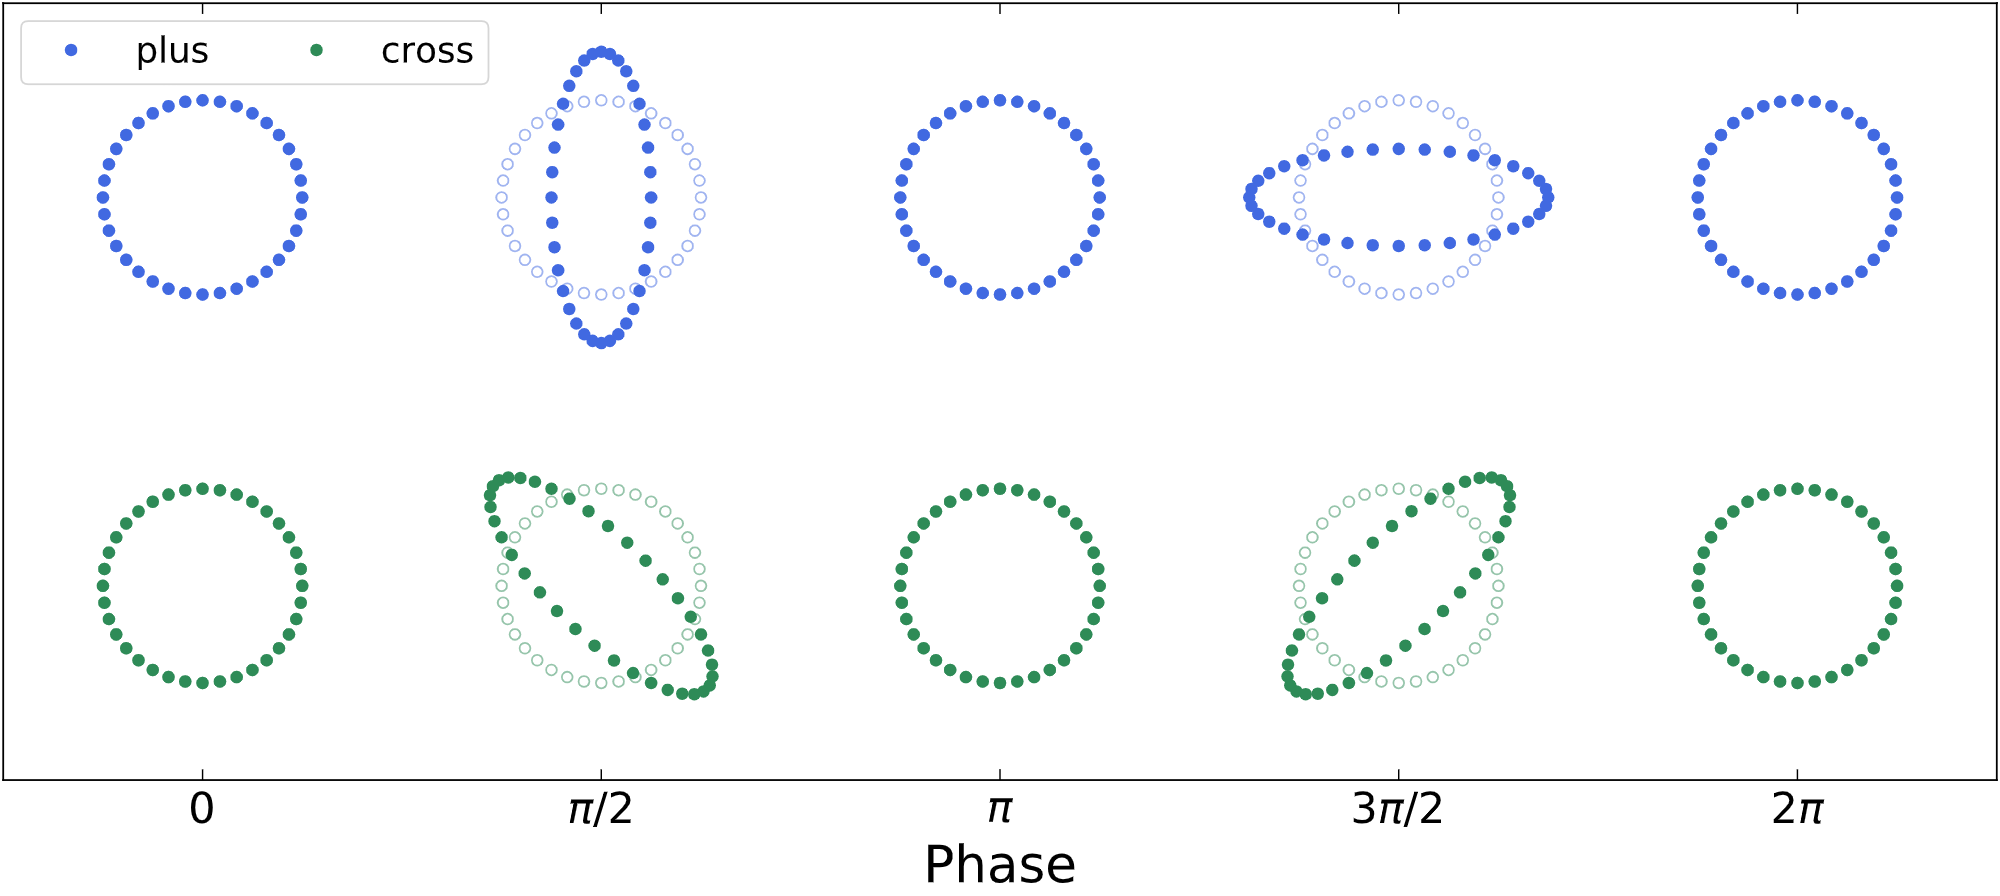
\includegraphics[width=\textwidth]{images/gr_gw/polarization.png}
   \caption{\label{fig:polarization}The effect of the two polarizations on a ring of test particles~\cite{gw_polarization_plots}.}
\end{figure}

A \gw polarized completely in the `plus' plane will produce a physical separation of any particle from the centre of the ring of:

\begin{equation}
   \Delta s = R[1 + \frac{1}{2} A_+ \cos(\omega t) \cos(2 \theta)]
   \label{eqn:plus_separation}
\end{equation}

Where $\Delta s$ is the physical separation of the particle from the centre, $R$ is the radius of the circle and, $\theta$ is the polar angle of each particle.

Likewise for a \gw completely polarized in the `cross' plane:

\begin{equation}
   \Delta s = R[1 + \frac{1}{2} A_{\times} \cos(\omega t) \sin(2 \theta)]
   \label{eqn:cross_separation}
\end{equation}

It is important to note that we are treating the separation between the particles and the centre in cartesian coordinates as the TT gauge is a comoving coordinate system where the coordinates of the particles are fixed
even as a \gw passes through.

\section{\label{sec:CBC}Gravitational Wave Sources - Compact Binary Coalescence}

A \cbc occurs when two stellar remnants, such as neutron stars (NSs) or black holes (BHs), in a binary system merge. This section will discuss \cbcs (CBCs) as a source of \gws.

The fraction of stars in binary systems is dependent on mass, research suggests that among very massive stars 80\% might be multiple-star systems \cite{binary_fraction}. This is important as we look for black-hole binary (BBH) systems as one of the CBC sources of \gws. It is also worth mentioning that while most binary systems will form that way, there is the potential for a dynamic capture to occur where compact objects are flung and caught from
their system to other systems; especially in highly dense stellar neighbourhoods such as the centre of galaxies \cite{dynamic_capture}.

The \gws we see from these objects are emitted continuously throughout their lifetimes. The orbit of the objects loses energy in the form of \gws, causing the radius of the orbit to decay. Over the course of billions of years the radius decays until the two objects merge. The \gw frequency is twice that of the orbital frequency \cite{kip_book} and we can determine the frequency sweep (the change in the frequency over time) using the equation (discarding higher order terms for simplicity):

\begin{equation}
   \frac{dF}{dt} = \frac{96}{5 \pi \mathcal{M}^2} (\pi \mathcal{M} F)^{\frac{11}{3}}
   \label{eqn:frequency_sweep}
\end{equation}

Where $F$ is the \gw frequency and $\mathcal{M}$ is the chirp mass: total mass, $M = m_1 + m_2$; reduced mass, $\mu = m_1 m_2/(m_1+m_2)$, symmetric mass ratio $\eta = \mu/M$ then $\mathcal{M} = \eta^\frac{3}{5} M$ \cite{PoissonWill}.

Equation \ref{eqn:frequency_sweep} shows that frequency of the \gw changes as a function of both the frequency and the chirp mass of the system. To higher order terms, the frequency evolution depends further on other parameters such as the spin-orbit and spin-spin parameter \cite{Will1993}.

For a BBH in a circular orbit, the evolution of the system will depend on 8 parameters: the two masses and six spin components. Further complexities such as neutron stars (non-rigid bodies) or eccentric orbits will require more parameters.

\section{\label{sec:IFOs}Gravitational Wave Detection}

The detection of \gws is made possible by \gw observatories: LIGO consists of Hanford \& Livingston \cite{aligo}; Virgo in Pisa \cite{avirgo}; KAGRA in Japan \cite{kagra}; and GEO in Germany \cite{geo}. This section will focus on
the design of the LIGO interferometers however, the techniques are similar for all detectors. The configuration of \aligo (aLIGO) is described in detail in the 2016 paper \cite{aligo}.

\subsection{\label{sec:laser_interferometry}Laser Interferometry}

As seen in section \ref{sec:Mechanics}, the effects of \gws in cartesian coordinates is a stretching and squeezing of the ring of test particles. We can measure this using laser interferometry allowing the detection of the small
perturbations caused by the presence of \gws in spacetime.

We begin with a basic L-shaped Michelson interferometer, seen in figure \ref{fig:basic_michelson}:

\begin{figure}
   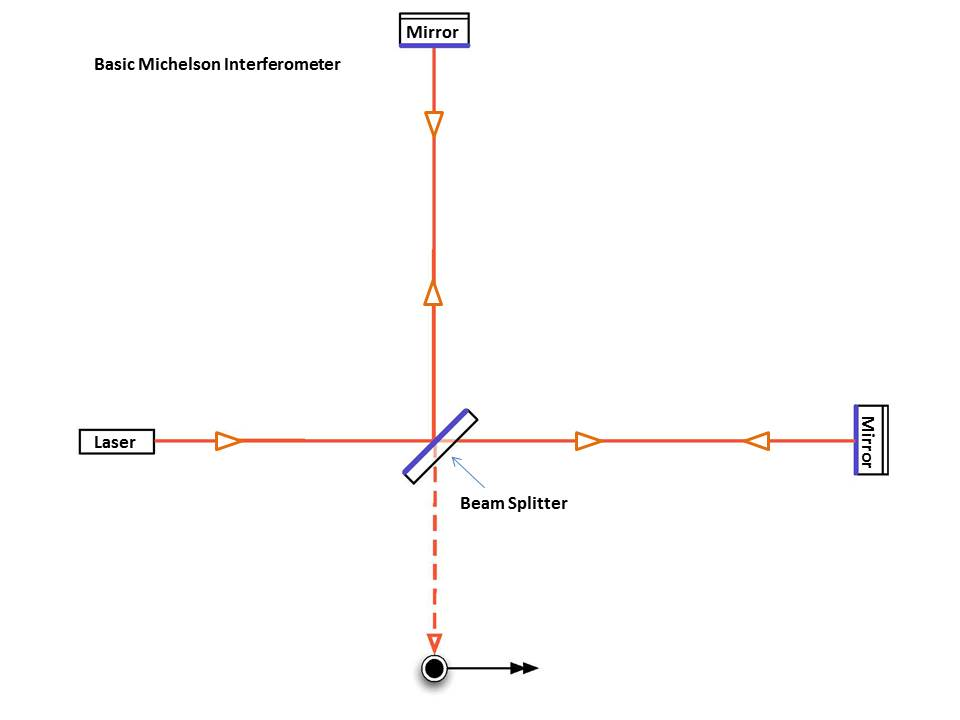
\includegraphics[width=\textwidth]{images/gr_gw/Basic_michelson_labeled.jpg}
   \caption{\label{fig:basic_michelson}A basic Michelson interferometer \cite{ligo_ifo}: A laser beam is shone at a beam splitter, the components are sent down equal length perpendicular arms where they reflect off the mirrors at the end, the components are then recombined back at the beam splitter and passed through to the photodetector (black circle) where the interference pattern of the laser is observed.}
\end{figure}

The LIGO detectors are identical in design with arm lengths of 4km, longer arms are able to make more precise measurements, looking at equations \ref{eqn:plus_separation} \& \ref{eqn:cross_separation}, the separation
$\Delta s$ depends on the radius $R$ (analogous to our arm length). We can further increase the distance our laser beam travels by using Fabry-Perot cavities to constantly recycle the laser in the arms. Figure \ref{fig:FP_michelson} shows the inclusion of Fabry-Perot cavities onto our basic Michelson interferometer.

\begin{figure}
   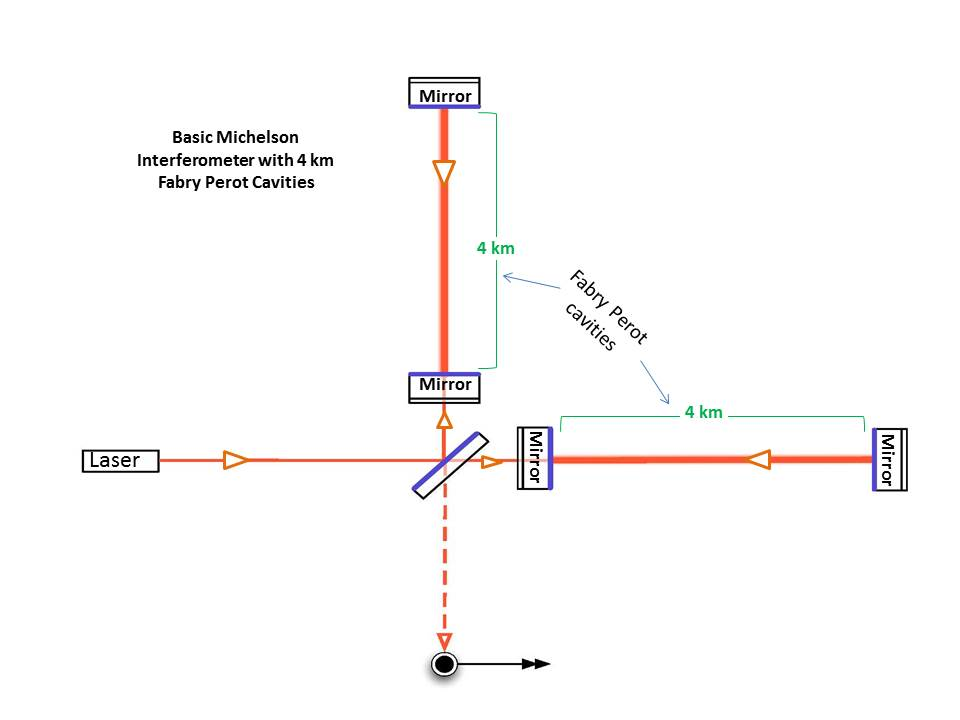
\includegraphics[width=\textwidth]{images/gr_gw/Basic_michelson_with_FP_labeled.jpg}
   \caption{\label{fig:FP_michelson}Fabry-Perot cavities \cite{ligo_ifo}: Additional mirrors are placed close to the beam splitter in each arm to allow the laser to traverse the arms many more times, effectively adding distance to our arms.}
\end{figure}

To create Fabry-Perot cavities extra mirrors are placed in each arm close to the beam splitter, these mirrors allow the laser to bounce back and forth within the arm many more times - effectively increasing the distance the laser has travelled. The Fabry-Perot cavities are fully evacuated, further reducing noise from the effects of interactions with particles in the air.

Laser power is continuously built up during this process, the more photons we have in our detector, the greater the resolution at our photodetector. We need to reach a laser power much higher than at the source, the Fabry-Perot
cavities don't provide enough amplification so we need to implement power recycling mirrors prior to the laser reaching the beam splitter. Some of the light from the laser is reflected towards the photodetector from the beam
splitter, the rest of it is sent back to the power recycling mirror. The power recycling mirrors can be seen in figure \ref{fig:IFO}.

\begin{figure}
   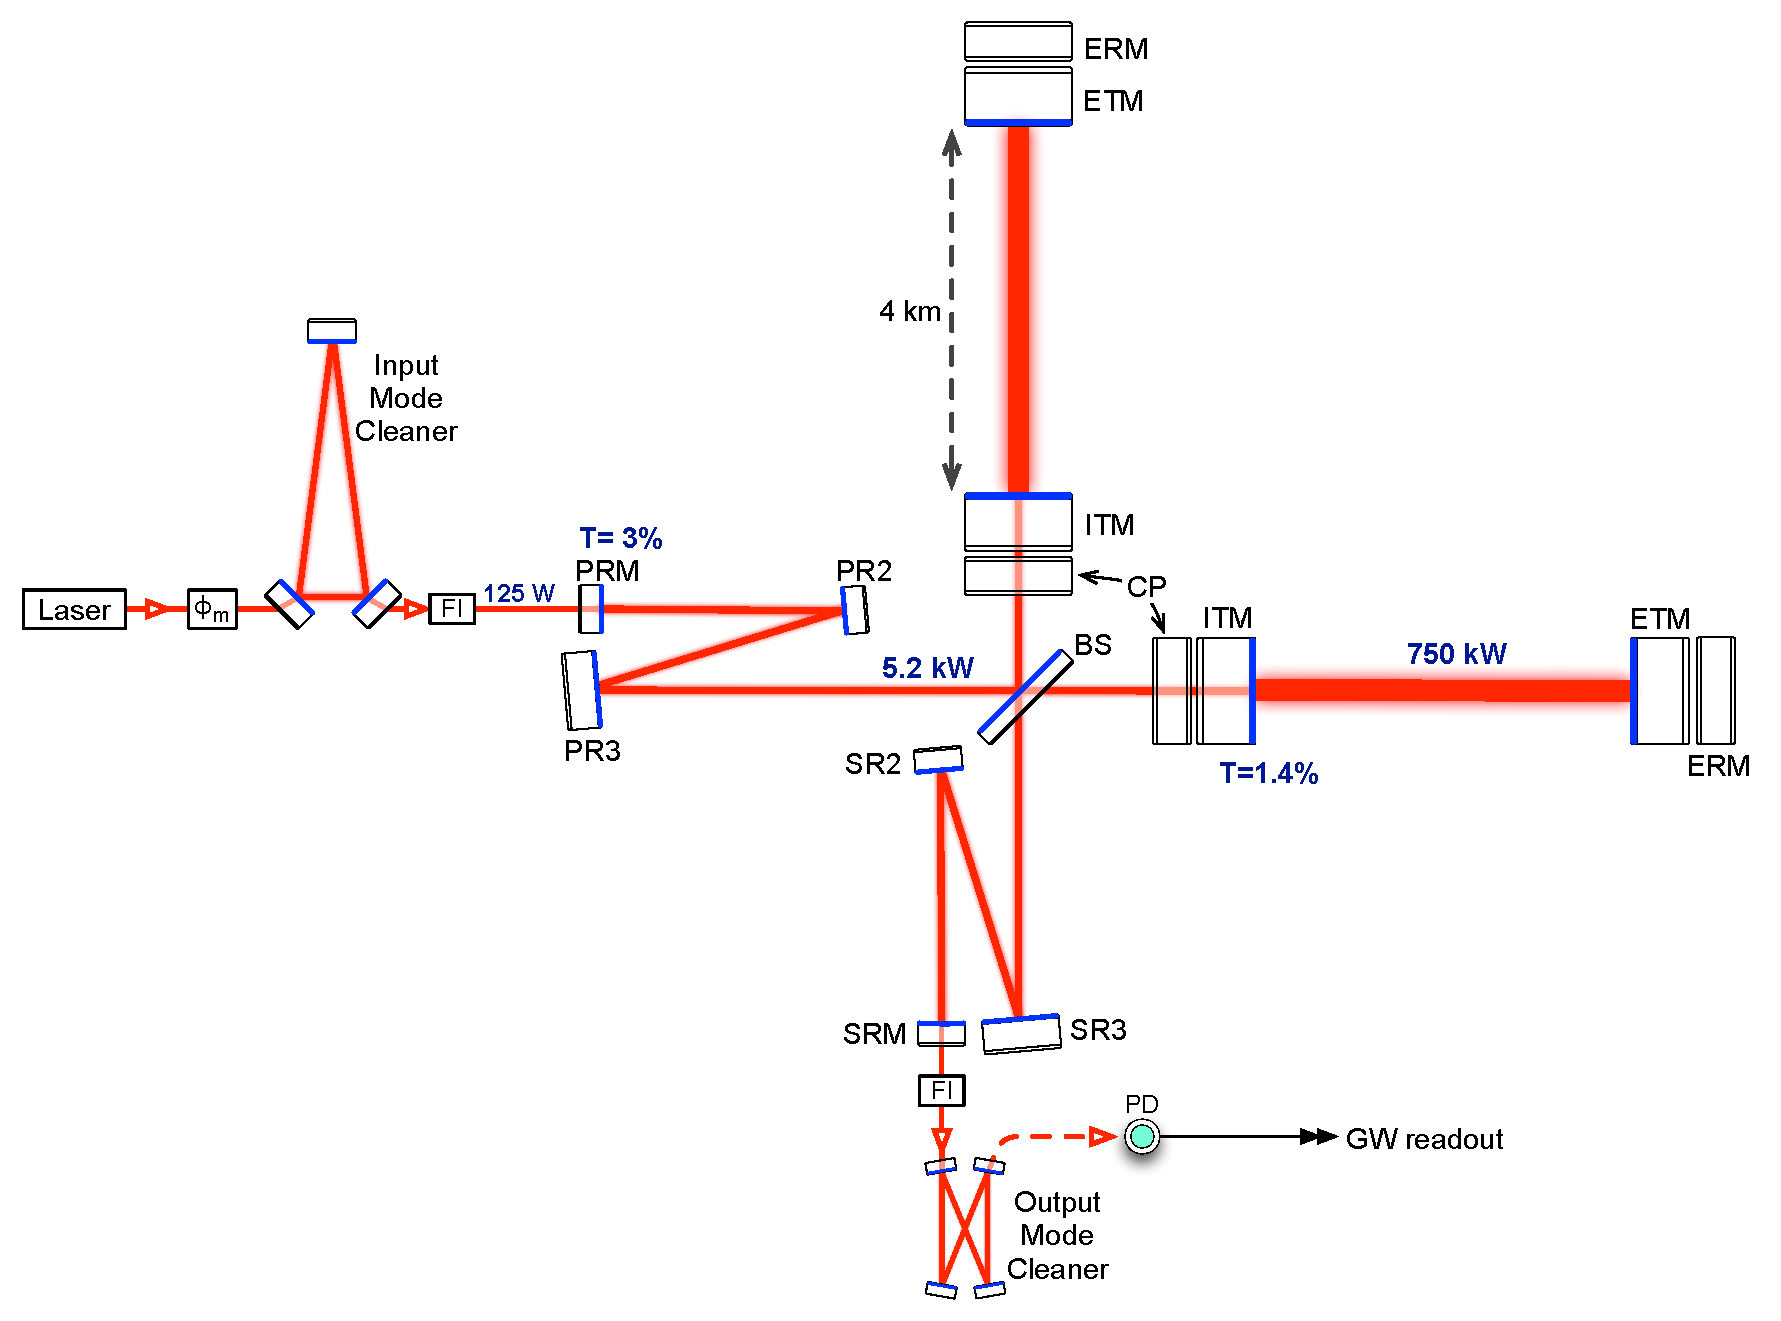
\includegraphics[width=\textwidth]{images/gr_gw/IFOdiagram.pdf}
   \caption{\label{fig:IFO}A more complex interferometer diagram \cite{aligo}: The Fabry-Perot cavities are formed by the input test mass (ITM) and end test mass (ERM) of each arm, the power recycling mirrors (PRM, PR2, PR3) appear prior to the beam splitter (BS)}
\end{figure}

Within the reference frame of the beam splitter and in the absence of \gws, the distance each laser travels up the arms is equal so that upon returning to the beam splitter, we see a constant interference pattern in the photodetector.
As a \gw propagates through the detector the beam splitter remains at rest but the mirrors at the end of each arm move (in our cartesian coordinate system), the lengths of the arms are now different and the recombination of the two beams will produce a phase difference upon returning back to the beam splitter \cite{thorne_lecture}.


%---% Searches %---%
\chapter{Searching for Gravitational Waves from Compact Binary Coalescence}
%%% CBC SEARCH %%%
% Search Methods
%   Gravitational Wave Data
%   Matched Filter
%   Phase Maximisation
%   Template Bank
%   Ranking Statistic
%       Coincident Detection
%       Signal-consistency tests
%       Template Fits
%       PSD Variation
% PyCBC Live Configuration
%   Low-Latency Detection
%   SNR Optimization
%   Ranking Statistic
%
Search pipelines, such as PyCBC Live, are used to analyse data from \gw detectors to detect \gw signals both in real-time (live) and afterwards (offline). In this chapter we introduce the techniques used by the PyCBC search pipelines to detect astrophysical signals buried in \gw data.

\section{\label{}Gravitational Wave Data}

\Gw data refers to that which is received from the gravitational wave detectors and is a time-series recording of the dimensionless strain measured by the detector for a stretch of time. The data, $s(t)$, is formed of a noise component, $n(t)$, and an astrophysical signal, $h(t)$, such that
%
\begin{equation}
    s(t) =
    \begin{cases}
        n(t), & \text{no signal} \\
        n(t) + h(t), & \text{signal}
    \end{cases}
\end{equation}

\section{\label{}Search Methods}
\Gws are difficult to find in \gw data due to the continuous parameter space and potentially infinite number of possible combinations of \gw signal parameters. In this section we will begin by briefly discussing how we model \gw waveforms in section~\ref{sec:waveform-modelling}, then we move onto signal processing techniques using these waveforms and the data in sections~\ref{sec:matched-filter}--\ref{sec:template-bank}.

\subsection{\label{sec:waveform-modelling}Waveform Modelling}

% Very brief
% Number of parameters
% Description of parameters

The waveform is composed using 15 parameters, split into intrinsic and extrinsic parameters. Intrinsic parameters describe physical properties of the system whereas extrinsic parameters describe things related to the detector network, position and/or orientation on the sky \cite{BAYEstar}.

Intrinsic parameters:
\begin{itemize}
   \item $m_1$, primary mass
   \item $m_2$, secondary mass
   \item $\vec{\chi_1}$, primary spin
   \item $\vec{\chi_2}$, secondary spin
\end{itemize}

Extrinsic parameters:
\begin{itemize}
   \item $\alpha$, right ascension
   \item $\delta$, declination
   \item $r$, distance
   \item $t_c$, time of coalescence
   \item $\iota$, inclination angle
   \item $\psi$, polarization angle
   \item $\phi_c$, coalescence phase
\end{itemize}

We create our waveform template using these parameters however, a bank of waveform templates in 15 dimensions will require an obscene number of templates to sufficiently cover. We can reduce the dimensionality by considering only signals which have no orbital precession or eccentricity. 

\subsection{\label{sec:matched-filter}Matched Filter}

Using GR, we can produce waveforms which represent a \gw in our photodetector output. Knowing what we are looking for allows us to use matched filtering, a signal processing technique where a known signal is correlated with data to
obtain a signal-to-noise ratio (SNR) informing us of the likelihood of the waveform being in the data

To being we can the data as a sum of a signal and noise:

\begin{equation}
   s(t) = h(t) + n(t)
   \label{eqn:s_h_n}
\end{equation}

Where $s$ is the data, $h$ is a signal (in this case, a real \gw signal) and $n$ is the noise. Using a template of the signal, we can use matched filtering to find the signal within our data.

The matched filter is defined as \cite{PyCBC_Search}:

\begin{equation}
   \rho^2(t) = \frac{(s|h)^2}{(h|h)}
   \label{eqn:matched_filter}
\end{equation}

The weighted inner product of the data, $s$, and the signal, $h$, in the frequency domain producing a signal-to-noise ratio (SNR), $\rho^2(t)$, in the time domain. We define the inner product:

\begin{equation}
   (s|h)(t) = 4 \Re \int^{+\infty}_{-\infty} \frac{\tilde{s}(f) \tilde{h}^*(f)}{S_n(f)} e^{2 \pi i f t} df
   \label{eqn:inner_product}
\end{equation}

A tilde, e.g. $\tilde{s}(f)$, denotes a Fourier transformed version of the variable.

\begin{equation}
   \tilde{s}(f) = \int^{+\infty}_{-\infty} s(t) e^{-2 \pi i f t} dt
   \label{eqn:fourier_transform}
\end{equation}

In equation \ref{eqn:inner_product} we have Fourier transformed data, $\tilde{s}(f)$, and a Fourier transformed signal, $\tilde{h}(f)$.

On the denominator within the integral in equation \ref{eqn:inner_product} $S_n(f)$ is the power spectral density (PSD) of the detector noise:

\begin{equation}
   \langle \tilde{n}(f) \tilde{n}(f') \rangle = \frac{1}{2} S_n(f) \delta(f-f')
   \label{eqn:PSD}
\end{equation}

The angle brackets denote averaging over noise realizations, $n$ is stationary Gaussian detector noise and $\delta$ is the Dirac delta function.

These equations build a tool that allows us to analyse a data to look for a signal. One requirement is that we must know the signal we are looking for before we search for it. We can create a template of our signal, referred to as a waveform. We then matched filter our data with the waveform and search through the resulting SNR timeseries for a peak, indicating the presence of the signal.

\subsection{\label{sec:phase-maximisation}Phase Maximisation}

Furthermore, the matched filter maximises the amplitude of the \gw signal and we have the ability to maximise over the phase of the signal by using an altered version of the matched filter:

\begin{equation}
   \text{$\rho^2_{\Phi,max}(t) = \frac{(s|h)^2 + (s|h_{\pi/2})^2}{(h|h)}$ where $\tilde{h}_{\pi/2}(f) = i \tilde{h}(f)$}
   \label{eqn:phase_mf}
\end{equation}

Where $\tilde{h(f)}$ and $\tilde{h}_{\pi/2}(f)$ are orthogonal phases of our template.

\subsection{\label{sec:template-bank}Template Bank}

Our waveform template bank will be only 5 parameters: the two masses, the two free spins and, the time of coalescence. We must create a bank of waveform templates describing all the possible signals and template density of the bank needs to be fine-tuned in order to ensure two things: our template bank covers the parameter space well enough to find all signals and our template bank isn't so large we are wasting computational time and resources \cite{Owen:tbank}.

\section{\label{sec:ranking-statistic}Ranking Statistic}
The ranking statistic is a measure of confidence that a signal originated from an astrophysical source as opposed to noise in the detectors. We use the ranking statistic to calculate a false alarm rate which informs us of the number of events per unit time that will originate from noise only. There must be a balance struck when choosing a false alarm rate at which events are determined to be real, require a very small false alarm rate and you will potentially exclude real events from a catalogue and allow too high of a false alarm rate and you will potentially include noise in the catalogue. In this section we will describe the different components which make up the ranking statistic.

%%%%%%%%%%%%%%%%%%%%%%%% TAKEN FROM PYCBCLIVE
Each trigger in an interferometer (H1 and L1) will produce an \verb|SNR| ($\rho$), $\chi^{2}$, $\chi^{2}$ degrees of freedom ($\chi^{2}_{dof}$) and Sine-Gaussian $\chi^{2}$ (\verb|sg_chisq|). To calculate the new SNR ($\rho_{new}$) for each trigger we must firstly convert $\chi^{2}$ to reduced-$\chi^{2}$ using the degrees of freedom which needs to itself be converted from the degrees of freedom saved in the Live trigger files:
%
\begin{equation}
\text{dof} = 2 \cdot \chi^{2}_{dof} - 2,
\end{equation}
%
\begin{equation}
  \chi_{reduced}^{2} = \frac{\chi^{2}}{\textrm{DOF}} = \frac{n}{2n - 2} \sum_{i=1}^n \left(\frac{\rho}{\sqrt{n}} - \rho_{bin,i}\right)^2.
  \label{eqn:chi_squared}
\end{equation}
%
\begin{equation}
\rho_{rw} =  \left\{  \begin{array}{l@{\quad}cr} 
\rho & \mathrm{if} & \chi_{r}^{2} < 1, \\  
\rho [(1 + (\chi_{r}^{2})^3)/2]^{-\frac{1}{6}} &  \mathrm{if} & \chi_{r}^{2} \ge 1,   
\end{array}\right.
\label{eqn:reweighting}
\end{equation}
%
\begin{equation}
\rho_{\text{new}} = 
\begin{cases} 
\rho_{\text{rw}} & \text{if } \text{sg\_chisq} \leq 4, \\  
\rho_{\text{rw}}  / \left(\frac{\text{sg\_chisq}}{4}\right)^{0.5} & \text{if } \text{sg\_chisq} > 4.
\end{cases}
\label{eqn:reweighting}
\end{equation}

Another consideration in the ranking statistic calculation when comparing the old statistic to the new statistic is how the $\rho_{new}$ for each detector is accounted for in the ranking statistic calculation. The old statistic is composed of two quantities, \verb|rstat|, which is the single detector $\rho_{new}$ and, \verb|logr_s|, which is the log of the expected signal rate. \verb|rstat| is calculated by summing the squares of the $\rho_{new}$ from each detector,
%
\begin{equation}
    \textbf{rstat} = \rho_{new, H1}^{2} + \rho_{new, L1}^{2}
\end{equation}
%
which then to find the total ranking statistic is added to $2 \times$ the log signal rate and square rooted,
%
\begin{equation}
    \textbf{cstat} = (\textbf{rstat} + 2 \cdot \textbf{logr\_s})^{\frac{1}{2}} \ .
\end{equation}
%
The new statistic simply takes the log signal rate, \verb|logr_s|, and subtracts the combined lognoiserate, \verb|ln_noise_rate|,
%
\begin{equation}
    \textbf{loglr} = \textbf{logr\_s} - \textbf{ln\_noise\_rate}
\end{equation}
%
where the combined lognoiserate is calculated in equation~\ref{eqn:pycbclive-combined-lognoiserate}.

We can directly compare how $\rho_{new}$ manifests in both of these equations. In the old statistic we are summing the squares of the $\rho_{new}$ from each interferometer and then square rooting after adding the contribution from the signal rate. In the new statistic we are simply adding the $\rho_{new}$ from each interferometer together (after applying the fits values). Due to this the old statistic will prefer higher SNR ratios between the two interferometers whereas the new statistic will favour equal SNRs.

For the old statistic, the quadrature sum of the SNRs will maximise the equation,
%
\begin{equation}
    a^{2} + b^{2} = (a + b)^{2} - 2ab
\end{equation}
%
where the difference between $a$ and $b$ is largest (neither $a$ or $b$ can be $0$ in our example because a coincidence detection requires both detectors to pass the minimum threshold). Therefore \verb|rstat| will be largest where the SNR ratio is greatest. In contrast, the new statistic will naturally favour equal SNRs as the search attempts to maximize the sum of the lognoises and not the squared sums when searching for coincidence pairs.

To visualise this difference we can plot the distribution of H1 and L1 SNR values and their coincident detector ranking statistic values. In both of these figures we neglect a changing signal rate and focus solely on the SNR contribution to the single detector ranking statistic.
%
%%%%%%%%%%%%%%%%%%%%%%%%%%%%%%%%%%%%%

\subsection{\label{sec:coincident-detection}Coincident Detection}

We want to see the same signal in more than one detector.

\subsection{\label{sec:signal-consistency-tests}Signal Consistency Tests}

We want the signal to follow the expected power distribution for that signal.

\subsection{\label{sec:template-fitting}Template Fitting}

When a template triggers with a large, we check to see if it commonly triggers with a large snr on noise historically. If it does then we can downweight our confidence that it is legitimate. If the template rarely ever triggers with a high snr on noise then we can increase our confidence in the detection.

We fit the distribution of triggers and snr to an exponential and the coefficient of the exponential is the number we use to weight.

How the fits are created:
- binning
- smoothing

\subsection{\label{sec:psd-variation}PSD Variation}

If the detector is behaving terribly we can model that and include it in the ranking statistic.

\subsection{\label{sec:kde-statistic} KDE Statistic}

\section{\label{sec:pycbc-live}PyCBC}

% Overarching points:
% - State of the field before my work
% - Overview of PyCBC Live in O3
% - Avoid talking about new developments

% What to talk about in this section:
% - Offline vs Live differences
% - Difference in computation of ranking statistic
% - How is ranking computed in Live
% -     Focus on methodology instead of code
% - O3 it wasn't able to cmopute some of the quantities that offline could
% -     Particularly things based on bulk statistics
% - Results in PyCBC Live being less sensitive
% -     List number of offline detections vs num live detections
% -     R&P paper demonstrated PyCBC Live is the most sensitive pipeline in all regions of parameter space in O3
% -     But gstlal had more events than pycbc (cross compare numbers and look at other pipelines)

% --------------------------------------------------

% Introduction to the section

This section combines the previously discussed techniques into an end-to-end pipeline used to detect gravitational waves. We will discuss primarily the PyCBC Live real time search for gravitational waves and how this search differs from the PyCBC offline search for gravitational waves including the limitations and the methodology differences to overcome these limitations.

\section{\label{sec:offline-vs-live}Offline vs Live}
% Differences in offline vs live

The search for gravitational waves occurs over two different time-scales. There is a "real-time" live search and an offline "post-detection" search, these searches have broadly the same goals--to detect gravitational waves--however they have different limitations, especially in the case of the live searches. Where the offline search has more time and potentially computing power available to probe the data more deeply, the live search is capable of rapidly sending information of potentially electromagnetically bright events to other astronomical observatories to perform multi-messenger astronomy.

PyCBC runs three searches currently for the fourth observing run, two live searches and an offline search. The live searches are the full-bandwidth complete template bank search which uses a template bank of \~730k templates to search for all known gravitational wave signals and, an early warning search which uses a much smaller \~9k template bank comprised of only electromagnetically bright frequency truncated signals intended to observe gravitational wave signals before the merger occurs. The third search currently running is the offline search which also uses a large bank of \~696k templates and want to observe all gravitational wave signals in the data.

This section will describe the PyCBC Live search in greater detail, focussing on the optimizations and unique components that differ it from the offline search and how these help to improve our detection of gravitational waves. The full bandwidth search is being described in these sections, the early warning search varies every so slightly but not enough to require distinctions to be made.

\subsection{\label{sec:low-latency-detection}Low-Latency Detection}

The PyCBC Live search aims to detect all gravitational waves in real time. This is a feat of software engineering to obtain the gravitational wave data, perform the matched filtering of hundreds of thousands of templates, perform signal consistency tests and output an approximate sky map within tens of seconds of the merger of the gravitational wave passing through the detectors.

The live search is distributed over 151 computing nodes and these are all connected through a message passing interface which tracks the individual search nodes. The main ranked node will receive messages from each of these nodes and distribute information and jobs to all the nodes. For example, when a node running a matched filter on H1 data finds a trigger and a node running a matched filter on L1 data finds a trigger, these triggers are sent back to the rank 0 node which then assigns another node to perform the coincidence tests as part of the ranking statistic to determine if this trigger was a real gravitational wave event.

The template bank of 730 thousand template distributed throughout the nodes and pre-generated in memory so the matched filters do not have to rely on generating the templates every time new data arrives. The template bank is shuffled into a random order so that the distribution of `long' and `short' templates is randomly distributed throughout the nodes. If a single node has all the long templates it will take longer to perform the matched filters than the nodes with the short templates and this can introduce lagging effects if the search is being held up by a single node.

The live search holds a continuous buffer of data where the newest eight seconds of data are added to the front and push the oldest eight seconds of data out of the buffer. The data is then matched filtered with the template bank and each node reports on the triggers that have been found. The hope with the search is that all of this processing can happen before the next eight seconds of data arrives at the detector. (PLOT: PYCBC LIVE LAG PLOT DIAGRAM THING)

\subsection{\label{sec:snr-optimization}SNR Optimization}

We upload potential detections of gravitational wave events to a central public database called GraceDB. These events are then used by astronomers to observe potential electromagnetic counterparts. We want to report the best information we can and produce the most accurate sky map. Increasing the SNR of the event is an easy way to improve this, having a better matching template to the signal will do this. (REWRITE).

The SNR optimization module of PyCBC Live takes a gravitational wave event and uses optimization functions to rapidly optimize the gravitational wave parameters to retrieve small fractions of improvement to the SNR. The original SNR of the event is limited by the template bank placement and the SNR optimizer allows a much finer exploration of the local parameter space to the best found template in the template bank. (ADD PLOT SHOWING TEMPLATE BANK WITH TEMPLATES NEARBY THE ACTUAL PARAMETER VALUES AND SNR IMPROVEMENT).

\subsection{\label{sec:live-ranking-statistic}Ranking Statistic}

The PyCBC Live ranking statistic run in the third observing run and the first half of the fourth observing run was very simple, only taking into account the Allen chisq, sine-gaussian chisq and phasetd. These are basic signal consistency tests for single detector checks, re-ranking the snr depending on how the morphology of the snr evolves over the signal. In coincidence the ranking statistic only looks for phase and template consistency for the two triggers and a time coincidence so that both detector triggers fall in light time travel time.



% Removed from pycbclive.tex
This chapter details the changes made to the PyCBC Live ranking statistic to improve on the original ranking statistic used in the third and fourth observing runs and detailed in~\ref{sec:live-ranking-statistic}. The two additions that were made to the ranking statistic were the inclusion of PSD variation, to track the non-stationary of the detector noise, and adding template fits to the statistic to weigh triggers based on their previously measured SNR distribution.

In this chapter we introduce the PyCBC Live search for CBC signals and the improvements made to the PyCBC Live search's ranking statistic to improve the sensitivity of the search and the confidence of our gravitational wave detections. The PyCBC Live search has been operational since the 2018~\cite{PyCBC_live} and has been in constant operation since, contributing to the 2nd, 3rd and 4th observing runs and detecting over 200 gravitational wave events. The PyCBC Live search processes gravitational wave detector data using techniques described in section~\ref{sec:Search} however, there are a number of optimizations and new techniques used to enable to low-latency rapid detection of gravitational wave events in close to real time.

PyCBC Live uses a ranking statistic post-detection of a gravitational wave event candidate which provides a numerical confidence in the event being real. This number is referred to as the `False Alarm rate' (FAR) and is measured in units of events per unit time (typically per year or Hertz). The inverse of the false alarm rate (IFAR) is commonly used and is typically measured in units of years. The false alarm rate tells us how often a candidate event would be observed due to random noise in the absence of a real astrophysical signal. IFAR can be thought of as the expected time interval between random noise events that could produce a signal resembling the observed candidate event. A higher IFAR indicates a longer expected waiting time between false alarms.

The LVK places a limit on the IFAR of a signal before it can be determined to be real. The limit has to be placed to balance the sensitivity of a search and the purity of a gravitational wave catalogue. As a quick example, if the IFAR limit is set to 1 year. Then one might expect to see one event per year in the catalog purely due to noise.

We begin this chapter by detailing the components that make up the ranking statistic and then the new components of the improved ranking statistic and how these are derived and used.

The layout of this chapter is as follows. In section~\ref{sec:live_optimizations} we detail the key components of t



%---% Detector Characterisation %---%
\chapter{Detector Characterisation}
The detector noise is approximated as Gaussian and stationary \cite{gaussian_noise}, this isn't true.
Data artefacts (commonly referred to as glitches) are non-Gaussian noise which inhibit the sensitivity of the
detector, reduce the quality of the data and, obscure \gw detections \cite{transient_noise}.

There are a number of common glitches in the detector data: blips \cite{blips}, whistles \cite{whistles},
scattered light \cite{Accadia}. The sources of these glitches are studied, for example, whistles are caused by the
beating of radiofrequencies in the detector, however, some glitches are from unknown sources (e.g. blips).

We can reduce the noise from the sources by making improvements to the detectors \cite{soni_scattered}, this lowers the
frequency of some glitches but doesn't remove them entirely. We can eliminate some glitches by completely removing the
source \cite{laura_char}. We are also able to reduce noise retroactively by gating certain times or using algorithms to
remove noise \cite{cit_science_soni}. An example of this is detailed in the section \ref{sec:scattered_light}.

%---% ArchEnemy %---%
\chapter{ArchEnemy}
I am first author on a peer-reviewer and published work carrying the name \textit{"ArchEnemy: Removing scattered-light glitches from gravitational wave data"}, within the Institute of Physics journal Classical and Quantum Gravity~\cite{ArchEnemy}.
\bibliographystyle{iopart-num}
\newcommand{\gguide}{{\it Preparing graphics for IOP Publishing journals}}
\newcommand{\gw}{gravitational wave}
\newcommand{\gws}{gravitational waves}
\newcommand{\Gw}{Gravitational wave}
\newcommand{\Gws}{Gravitational waves}
\newcommand{\scl}{scattered-light}
\newcommand{\Scl}{Scattered-light}

\section{\label{sec:ArchEnemy-intro}Introduction}

The Laser Interferometer Gravitational-Wave Observatory (LIGO)~\cite{aligo} and Virgo~\cite{avirgo} collaborations made the first observation of \gws{} in September 2015~\cite{first_detection}. The detection established the field of \gw{} astronomy and a global network of \gw{} detectors, now joined by KAGRA~\cite{kagra}, has allowed for the detection of approximately 100 \gw{} events~\cite{gwtc1, gwtc2, gwtc21, gwtc3}.

The detection of \gws{} is made possible by both the sensitivity of the detectors and the search pipelines~\cite{pycbc, gstlal, spiir, mbta, cwb_2020} which analyse raw strain data from the output of the detectors and identify observed \gw{} signals. One of the problems that these search pipelines must deal with is the fact the data contains both non-stationary noise and short duration `glitches'~\cite{GuideToDetNoise,DetCharO2O3, VirgoDetChar} where noise power increases rapidly. Glitches are caused by instrument behaviour or interactions between the instrument and the environment~\cite{transient_noise, Glanzer:2023hzf} and glitches reduce the sensitivity of the detectors~\cite{sensitivity_o3}, can potentially obscure candidate \gw{} events~\cite{gwtc2} and can even mimic \gw{} events~\cite{GWMimicking, PyCBC_Singles}.

Different classes of glitches have been characterized using tools such as Gravity Spy~\cite{gravityspy, GSpy_update}. Of the 325,101 glitches classified by Gravity Spy in the third observing run of Advanced LIGO~\cite{GSpy2022} with a confidence of $90\%$ or higher, 120,733 ($32.1\%$) were classified as ``Scattered Light''. \Scl{} glitches occur in the 10-120Hz frequency band~\cite{reducing_scattering_o3} which coincides with the frequency band where we observe the inspiral and merger signatures of compact binary coalescences. \Scl{} glitches are characterized by an arch-like pattern in a time-frequency spectrogram of the detector output, as seen in figure~\ref{fig:scattered_light}. 
%
\begin{figure}
  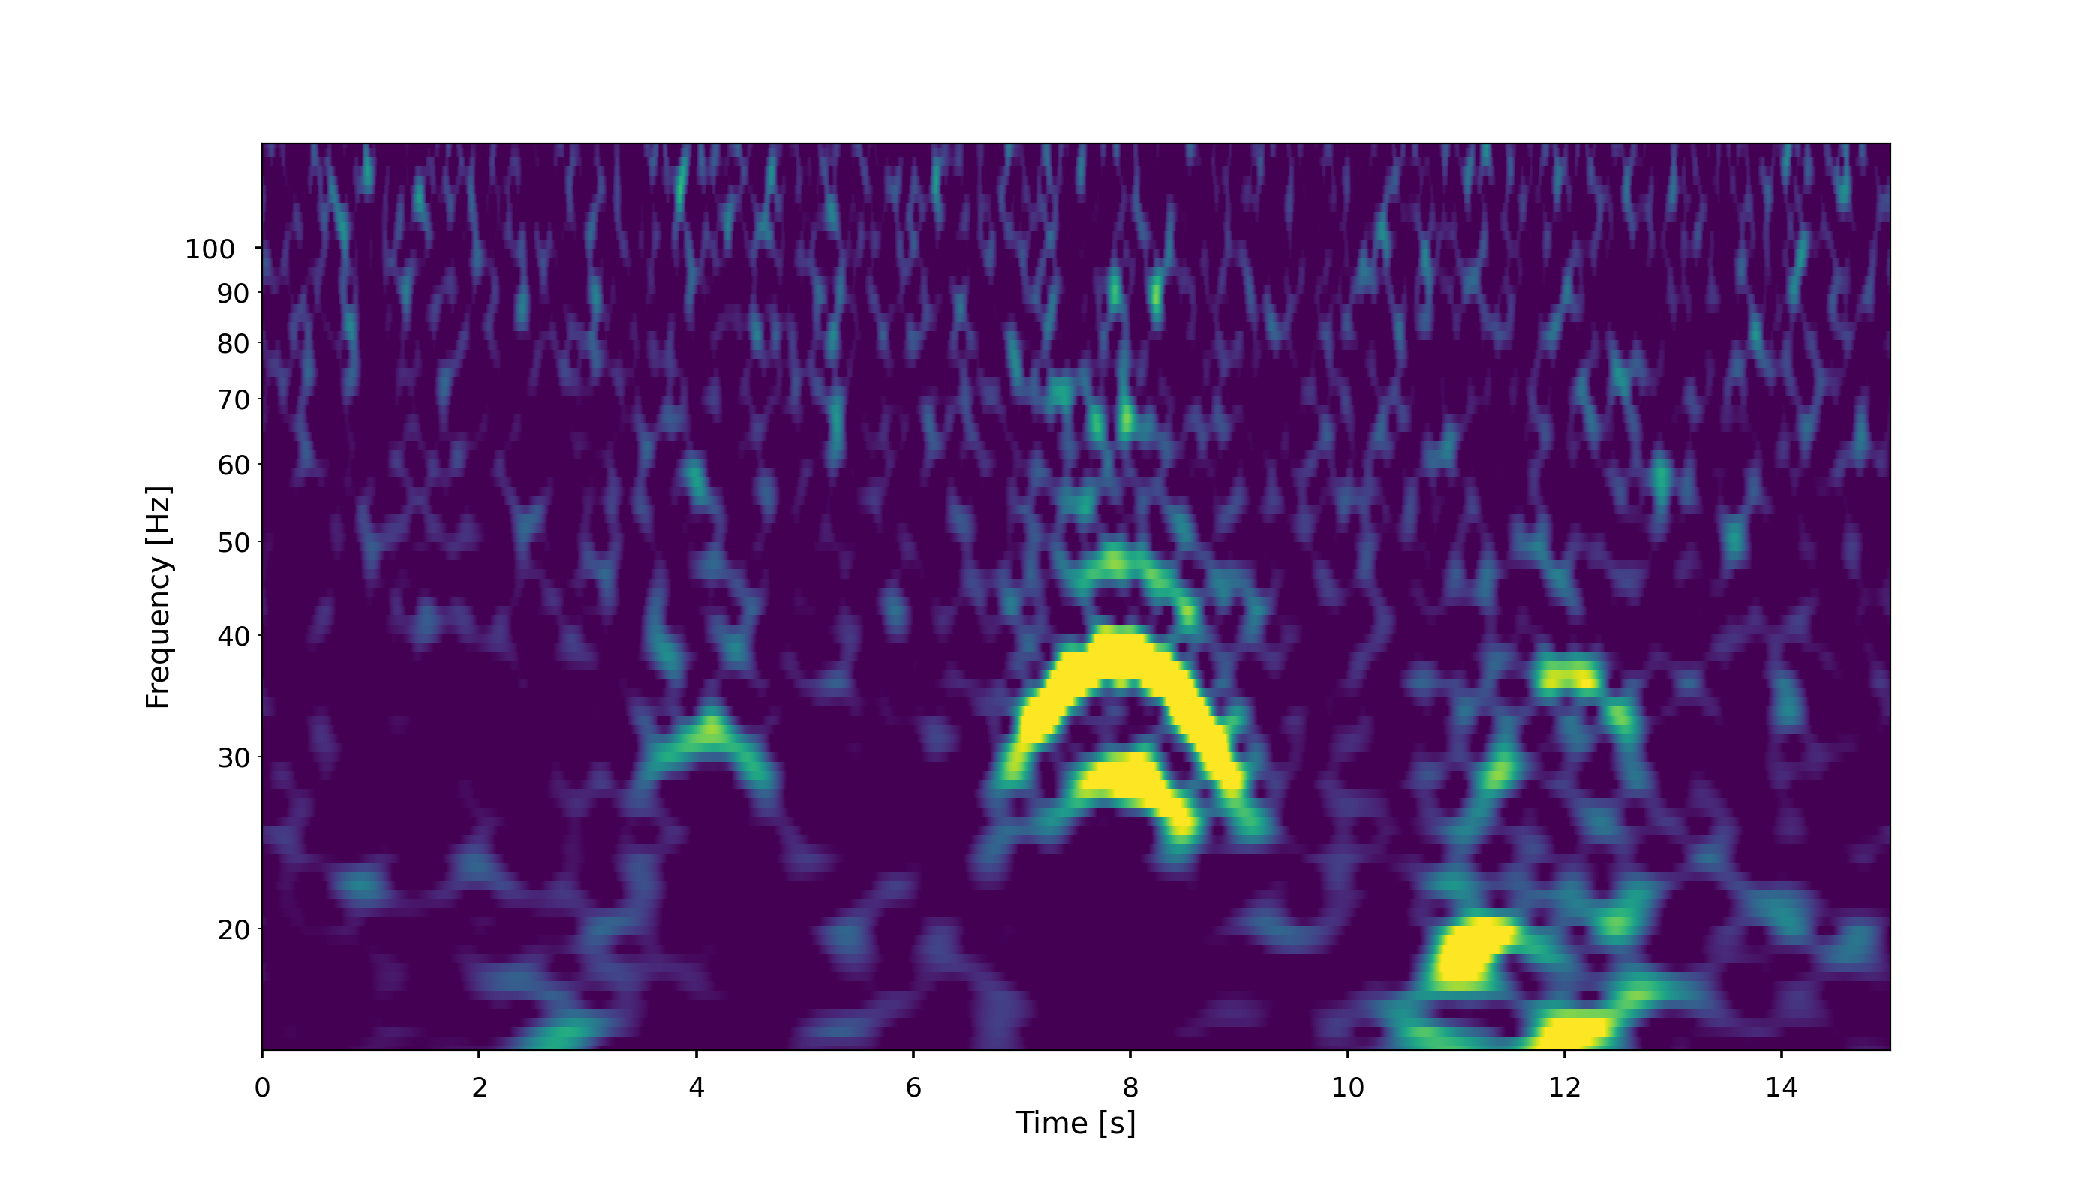
\includegraphics[width=\textwidth]{Figures/Section1/single_stack.pdf}
  \caption{An Omega scan \cite{omegascan} of \gw{} data containing an example of a \scl{} glitch. \Scl{} glitches are characterized by a symmetric arch-like pattern. Multiple \scl{} glitches can be seen at the 4, 8 \& 12 second marks as well as multiple harmonic glitches at 8 seconds.}
  \label{fig:scattered_light}
\end{figure}
%
\Scl{} glitches occur when laser light in the interferometer is scattered from the main optical path by components within the detector. The motion of these components is coupled to seismic motion inducing a phase shift on the light being scattered as the surface moves back and forth. This \scl{} then recombines with the main laser, producing \scl{} glitches in the data. The surfaces from which \scl{} glitches originate have been objects on optical benches such as lenses, mirrors and photo-detectors~\cite{TAccadia}.

\Scl{} glitches have been a significant problem when observing compact binary mergers. As an example, GW190701\_203306 was coincident with a \scl{} glitch, as shown in figure \ref{fig:obscured_detection}~\cite{gwtc2}, requiring subtraction from the data before the event could be properly characterized~\cite{O3_subtraction}. A further 7 candidate events were found to be in coincidence with \scl{} glitches in the third observing run~\cite{gwtc3}. For this reason, it is important to reduce the effect of \scl{} glitches in the detectors and \gw{} search pipelines. \Scl{} glitches occur as single or multiple glitches and can appear rapidly in time and simultaneously in frequency (see figure \ref{fig:consec_scattered_light}), which we refer to as harmonic glitches.

\begin{figure}
  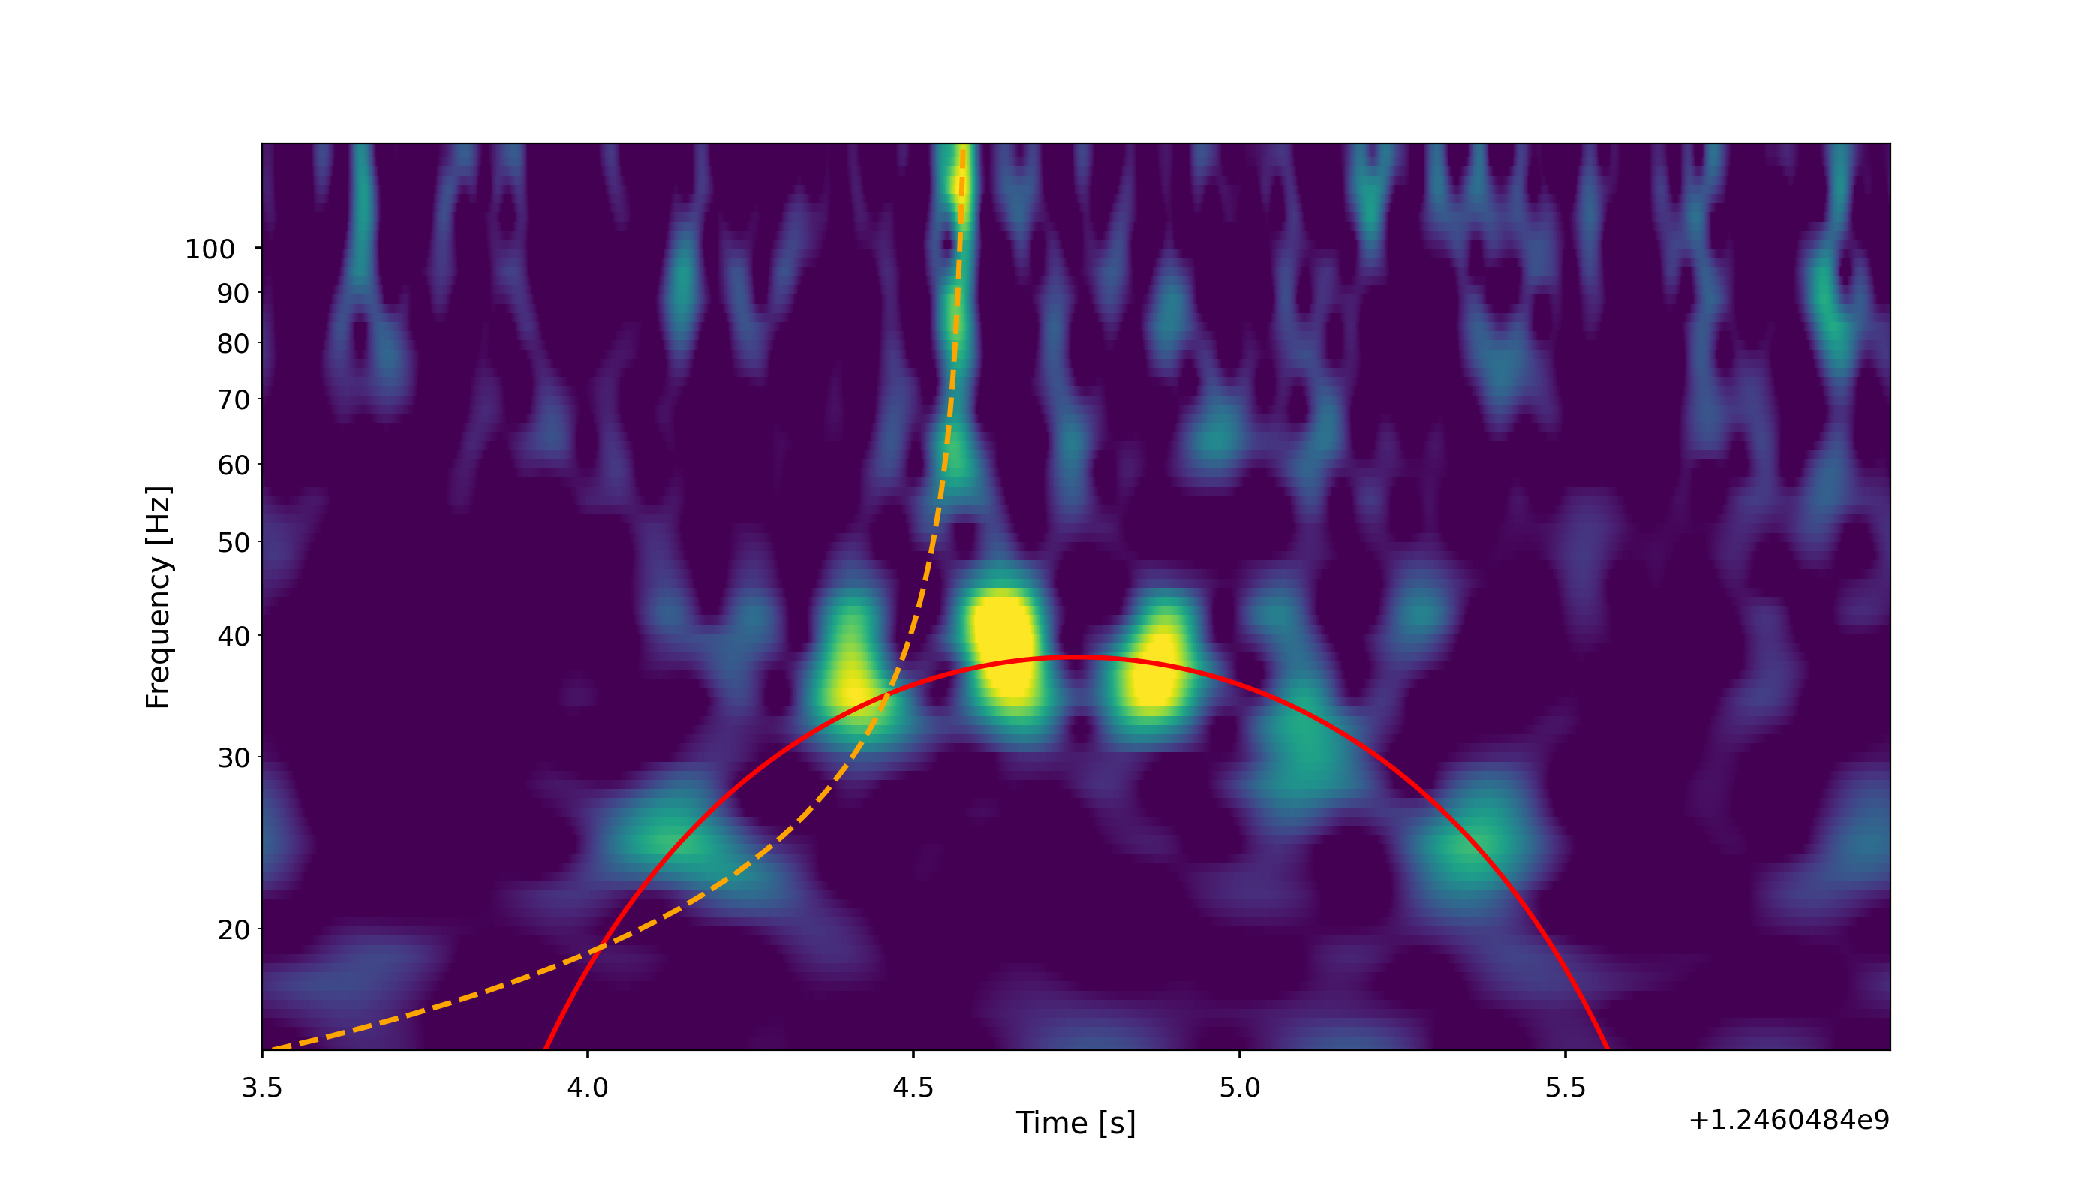
\includegraphics[width=\textwidth]{Figures/Section1/GW190701_203306_overlay.pdf}
  \caption{GW190701\_203306, a \gw{} event coincident with a \scl{} glitch in the data from the LIGO Livingston observatory. The orange dashed track shows the inferred time-frequency evolution of a \gw{} event produced by a compact binary merger, the red solid line is an overlaid track of the approximate location of the coincident fast scattering glitches.}
  \label{fig:obscured_detection}
\end{figure}

\begin{figure}
  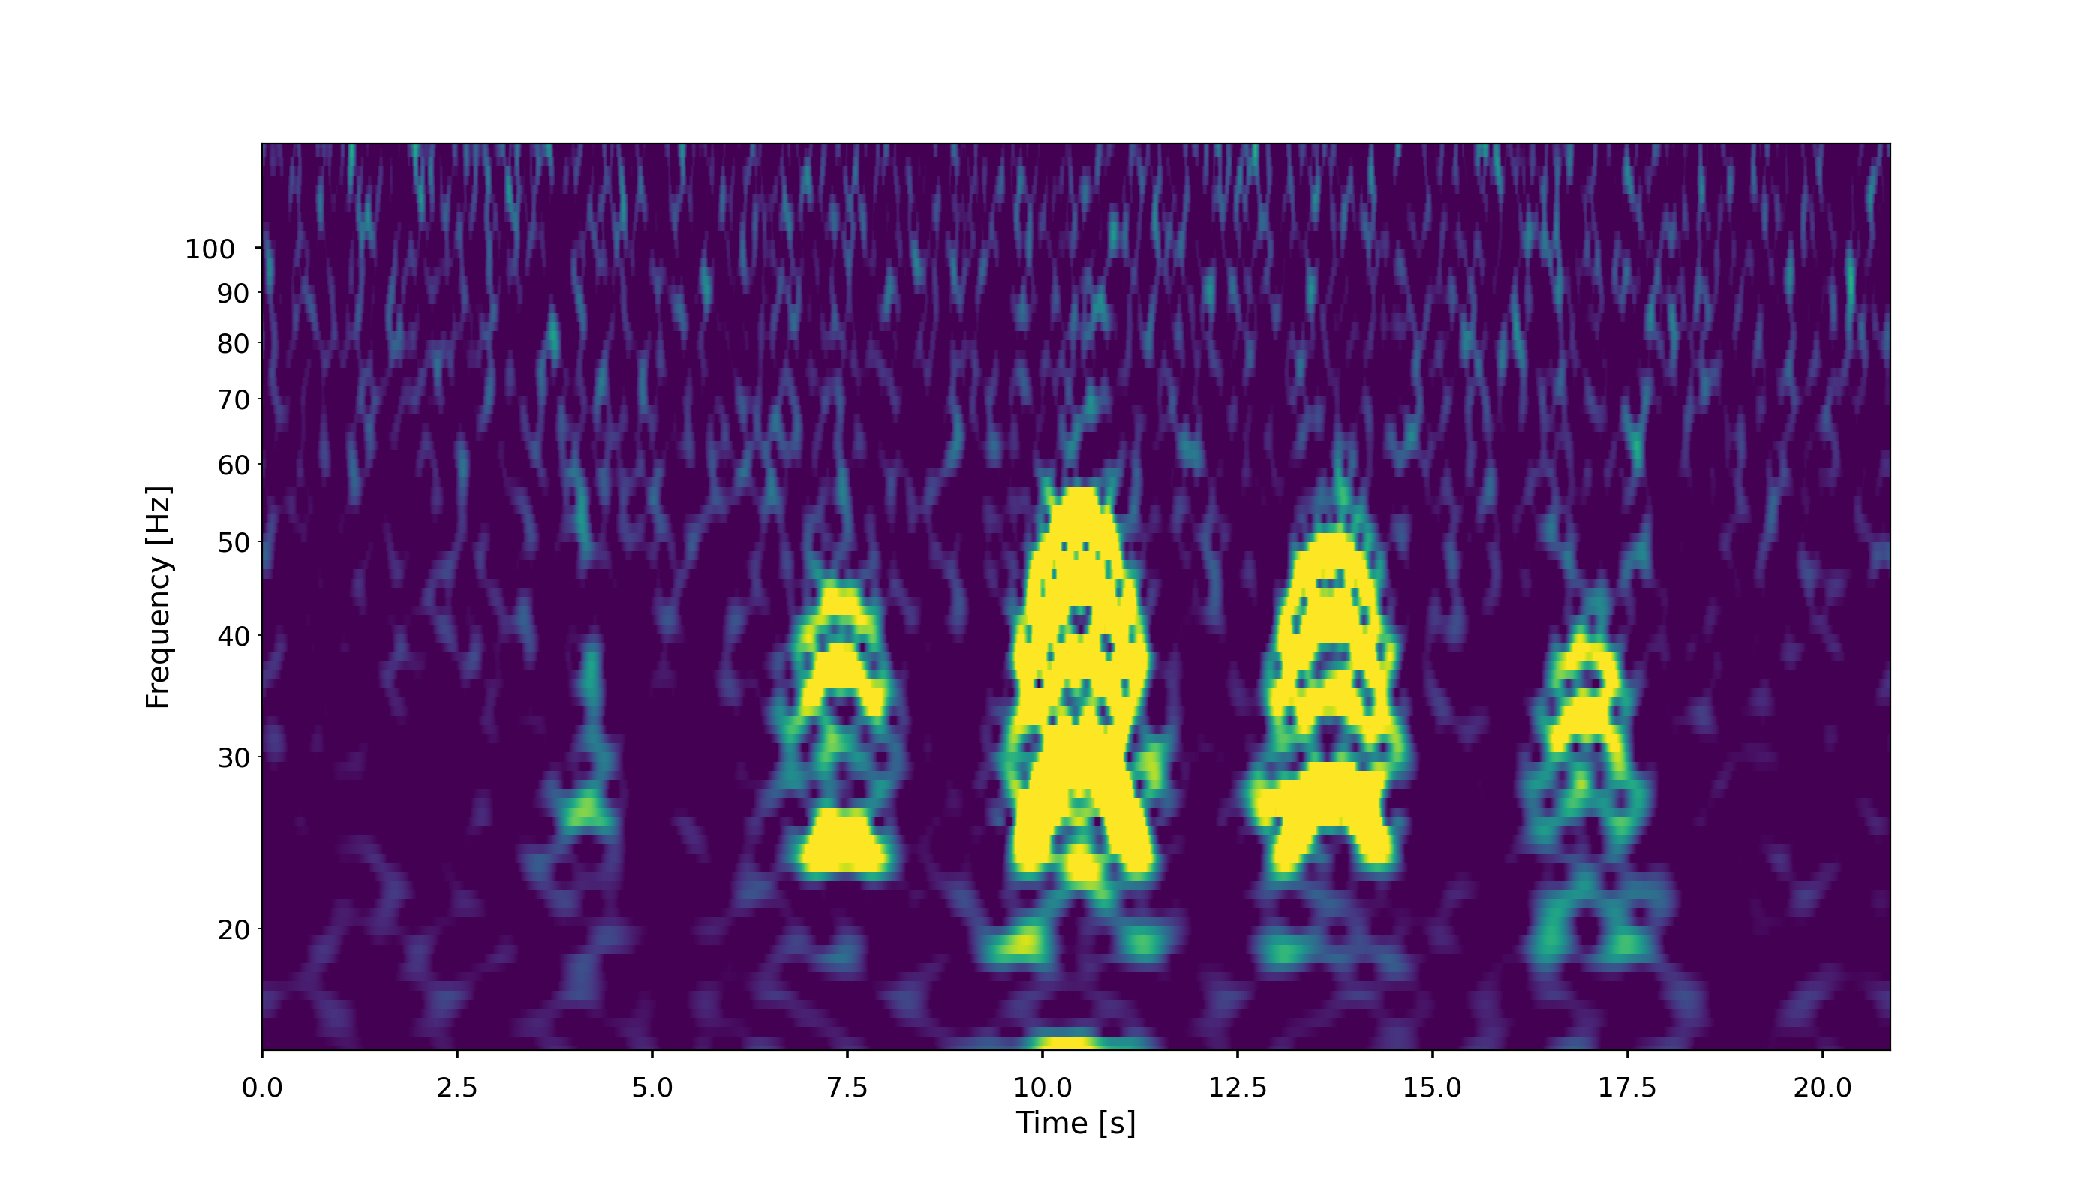
\includegraphics[width=\textwidth]{Figures/Section1/multiple_harmonics.pdf}
  \caption{An Omega scan \cite{omegascan} of \gw{} data containing multiple examples of \scl{} glitches. Here we see multiple \scl{} glitches repeating periodically in a $20$ second period of time. Harmonic \scl{} glitches are also seen in multiple stacks, the harmonic glitches share \emph{time period} values and the \emph{glitch frequency} values are $n-$multiples of the lowest frequency harmonic within the stack.}
  \label{fig:consec_scattered_light}
\end{figure}

The most obvious way to remove the impact of glitches is removing the mechanisms which produce the glitches in the observatories. This has been investigated in previous works~\cite{reducing_scattering_o3, TAccadia, Laura_Noise, gwadaptive, HilbertHuang, tvf-EMD, Longo_daily, MichalSub}, which focus on identifying the surfaces in which light is being scattered from and then mitigating the scattering by reducing the reflectivity of the surface, seismically isolating it or relocating it. 

An alternative method for reducing \scl{} glitches, known as ``RC tracking'', was implemented in the Advanced LIGO observatories in January 2020~\cite{reducing_scattering_o3}. The Advanced LIGO detectors employ a quadruple pendulum suspension for the test masses where two chains suspend four masses in this suspension system, one for the test mass optic and the other for the reaction mass. The reaction mass is used to impose a force upon the test mass and a significant source of \scl{} glitches was the large relative motion between the test mass chain and the reaction chain. To mitigate this effect, the relative motion between the end test mass and the reaction mass needed to be reduced. This was achieved by ensuring the two chains are moving together by applying force to the top stage of the quadruple suspension system in Advanced LIGO. The implementation of RC tracking represented a decrease from $0.01 s^{-1}$ to $0.0001 s^{-1}$ and $0.0072 s^{-1}$ to $0.0012 s^{-1}$ in the number of \scl{} glitches detected by Gravity Spy for LIGO-Hanford and LIGO-Livingston respectively.

While methods for preventing \scl{} glitches have been developed and have shown success, they have not been able to remove the problem of \scl{} glitches from the data. Additionally, as the detectors continue to be upgraded and increase in sensitivity, new sources of \scl{} glitches will continue to appear. Identifying these new sources and mitigating their effects can take many months, during which time the detectors are taking in data which might be affected by the presence of \scl{} glitches. Therefore, it is not realistic to believe that analyses will be able to regularly run on data that does not contain \scl{} glitches and this motivates us to develop a technique for mitigating the impact of these glitches when trying to identify compact binary mergers in \gw{} data.

In this work we present a new method for identifying and removing \scl{} glitches from \gw{} data in advance of running searches to identify compact binary mergers.
We first introduce a method for identifying when \scl{} glitches are present in detector data, through the creation of a new modelled search for \scl{} glitches, similar to how we search for \gws{} using matched filtering. We can model \scl{} glitches, generate a suitable set of glitch waveforms and perform a matched filter search on detector data. We then subtract identified glitches from the data to increase detector sensitivity. The detector data isn't Gaussian and stationary so the matched filter does have the potential to identify non-\scl{} glitches, and potentially even \gw{} signals, as \scl{} glitches. To prevent this we also demonstrate a new \scl{} $\chi^{2}$ test, which can distinguish between \scl{} glitches, and other glitches---and \gw{} signals---in the data.

We begin by reviewing previous research and describing the formulation of the waveform model used for characterizing \scl{} glitches in section \ref{sec:sc_li}. In section \ref{sec:search_techniques} we introduce the various techniques used in the search to identify \scl{} glitches in \gw{} data and the results of the \scl{} glitch search. In section \ref{sec:results} we describe the results of a ``glitch-subtracted'' \gw{} search and any increases in sensitivity. We conclude in section \ref{sec:conclusion} and discuss the implementation of this method in future observing runs.

\section{\label{sec:sc_li}\Scl{}}

To identify \scl{} glitches in \gw{} data requires an accurate model of \scl{} glitches. This section details the derivation of the model we will use for generating our \scl{} glitch filter waveforms, along with its parameterization.

\subsection{Modelling \scl{} glitches - a review}

Our model for \scl{} glitches draws heavily from~\cite{TAccadia}, and we briefly review the main details of the model presented there. In~\cite{TAccadia}, the authors construct a model to accurately predict the increase in noise due to \scl{} during periods of increased micro-seismic activity. The model in~\cite{TAccadia} is constructed from parameters related to physically measurable properties of the detector such as the mirror transmission factor, $T$, the finesse of the Fabry–Pérot cavity, $F$, or the wavelength of the light, $\lambda$.

They define the amplitude of the additional beam produced by light scattering off of a surface as
%
\begin{equation}
    A_{sc} = A_{0} T \sqrt{\frac{2 F}{\pi}} \sqrt{f_{sc}} e^{i \phi_{sc}}\,,
    \label{eqn:accadia_amplitude}
\end{equation}

%
where $A_{0}$ is the amplitude of the light resonating in a Fabry–Pérot cavity, $f_{sc}$ is the fraction of the optical power scattered back into the main beam and $\phi_{sc}$ is the phase angle modulated by the displacement of the scattering optics, defined as
%
\begin{equation}
    \phi_{sc}(t) = \frac{4 \pi}{\lambda} ( x_{0} + \delta x_{opt}(t) ),
    \label{eqn:accadia_phase_noise}
\end{equation}
%
where $\delta x_{opt}$ is the displacement of the scattering surface and $x_0$ is the static optical path.

The total amplitude of the beam inside the arm is given by $A_{tot} = A_{0} + A_{sc}$, with a phase angle equal to the phase noise introduced by the \scl{} $\delta \Phi = \frac{A_{sc}}{A_{0}} \cdot \sin \phi_{sc}$. The noise introduced by the \scl{}, $h_{sc}$, can be approximated through the relationship $\sin(\Phi_0+ \delta\Phi) \approx \cos(\Phi_0) \times \sin(\delta \Phi)$ for small $\delta\Phi$, and can be expressed as
%
\begin{equation}
    h_{sc}(t) = G \cdot \sin \left(\frac{4 \pi}{\lambda} (x_{0} + \delta x_{sc}(t) ) \right),
    \label{eqn:accadia_strain}
\end{equation}
%
where $G$ is the \emph{coupling factor}, defined as $K \cdot \sqrt{f_{sc}}$ where
%
\begin{equation}
K = \frac{\lambda}{4 \pi} \frac{T}{\sqrt{2 F \pi}}.
\end{equation}
%

The displacement of the scatterer when presenting with oscillatory motion is then given as
%
\begin{equation}
    \delta x_{sc} (t) \simeq A_{m} \sin(2 \pi f_{m} t),
    \label{eqn:accadia_oscillatory}
\end{equation}
%
where $f_{m}$ is the frequency-modulated signal with modulation index $m = A_{m} \frac{4 \pi}{\lambda}$ and where $A_{m}$ is the amplitude of the $n$th harmonic. Finally, equation~\ref{eqn:accadia_strain} can be simplified when considering only small bench motion, according to
%
\begin{equation}
    h_{sc}(t) = G \cdot \cos\phi_{0} \cdot \frac{4 \pi}{\lambda} \cdot \delta x_{sc}(t) \;.
    \label{eqn:accadia_strain_linearized}
\end{equation}

\subsection{Model}

The model introduced in~\cite{TAccadia} for the \gw{} strain noise introduced by \scl{} uses a lot of knowledge about the detector state. The model used in this work will be more phenomenological in the parameterization, allowing us to rely only on the characteristics of the glitches in the strain data and not knowledge of the detector configuration, especially in cases where this detector information might not be known. Each \scl{} glitch, as viewed in a spectrogram (see figure \ref{fig:scattered_light}), has two easily identifiable features: the maximum frequency reached, \emph{glitch frequency} ($f_{gl}$); and the period of time the glitch exists in detector data, \emph{time period} ($T$).  In addition we can fully describe an artifact by defining an \emph{amplitude} ($A$), \emph{phase} ($\psi$) and \emph{center time} of the glitch ($t_0$).

To formulate a model of \scl{} glitches in terms of these parameters, we simplify equation \ref{eqn:accadia_strain_linearized}, treating the strain noise caused by \scl{} as the sinusoidal function
%
\begin{equation}
  h_{sc}(t) \propto \sin(\phi_{noise}(t)).
  \label{eqn:h_sc_initial}
\end{equation}
%
Here the induced phase noise ($\phi_{noise}$) is equal to 
%
\begin{equation}
    \phi_{noise}(t) = 2 \pi f_{rep} t,
     \label{eqn:phi_noise}
\end{equation}
%
and $f_{rep}$ is the frequency of repetition of the sinusoid and is directly related to the \emph{time period}, $T$,
%
\begin{equation}
  f_{rep} = \frac{1}{2 T}.
  \label{eqn:f_rep}
\end{equation}
%
The \emph{time period} of a \scl{} glitch only corresponds to half of a sinusoidal wave hence the multiplier of 2 on the denominator of equation \ref{eqn:f_rep}.

\Scl{} glitches are caused by the physical increase in the distance travelled by the light as a consequence of being reflected off of a surface. The light returning to the beamsplitter from one arm will have travelled a different path length compared to the other arm and this path difference will act as a phase difference between the two arms causing non-destructive interference. The path difference and phase difference can be related with
%
\begin{equation}
  \Delta \phi_{scattering}(t) = 2 \cdot \frac{2 \pi}{\lambda} \Delta x(t),
  \label{eqn:delta_phi_scat}
\end{equation}
%
where $\Delta x(t)$ indicates the change in the path taken by the light over time. An additional multiplier of 2 indicates our path difference is occurring twice, once when the light approaches the surface and again when leaving.

We assume the scattering surfaces are oscillatory in motion and apply the same simplification made in equation \ref{eqn:accadia_oscillatory}, with an initial position $\Delta x = 0$ to a maximum displacement of $x_{0}$. This produces an equation for the path difference of the light,
%
\begin{equation}
  \Delta x(t) = x_{0} \sin(2 \pi f_{rep} t).
  \label{eqn:delta_x_t}
\end{equation}
%
We substitute equation \ref{eqn:delta_x_t} into equation \ref{eqn:delta_phi_scat} and produce an equation for the phase noise induced by \scl{}
%
\begin{equation}
  \phi_{scattering}(t) = \frac{4 \pi}{\lambda} x_{0} \sin(2 \pi f_{rep} t) \;,
  \label{eqn:phi_sc}
\end{equation}
%
this equation for the phase noise induced by \scl{}, $\phi_{scattering}(t)$, and the equations for the generic phase noise, $\phi_{noise}(t)$ (equation \ref{eqn:phi_noise}), can now be used to create an equation for the strain noise caused by \scl{}.

We take the derivatives of equations \ref{eqn:phi_noise} $\&$ \ref{eqn:phi_sc} with respect to time:
%
\begin{equation}
  \phi_{noise} ^\prime (t) = 2 \pi F_{inst} (t),
\end{equation}
%
\begin{equation}
  \phi_{scattering} ^\prime (t) = \frac{4 \pi}{\lambda} x_{0} 2 \pi f_{rep} \cos(2 \pi f_{rep} t) \;,
\end{equation}
%
where $F_{inst}$ is the instantaneous frequency at a specific time. We generate \scl{} glitches from $\frac{-T}{2}$ to $\frac{T}{2}$ to ensure their maximum frequency occurs at $t = 0$. We define this maximum frequency as the \emph{glitch frequency}.

We equate the two derivatives and set $t = 0$, this replaces $F_{inst}(t)$ with $f_{gl}$ and $\cos(2\pi f_{rep} t)$ with $1$, then re-arrange to find the maximum displacement of the scattering surface, $x_{0}$, as
%
\begin{equation}
  x_{0} = \frac{f_{gl}}{f_{rep}} \frac{\lambda}{4 \pi}.
  \label{eqn:x0}
\end{equation}
%
Substituting equation \ref{eqn:x0} into equation \ref{eqn:phi_sc} gives us an expression for the \scl{} phase noise,
%
\begin{equation}
  \phi_{scattering}(t) = \frac{f_{gl}}{f_{rep}} \sin(2 \pi f_{rep} t),
  \label{eqn:phi_sc2}
\end{equation}
%
and substituting equation \ref{eqn:phi_sc2} as our $\phi_{noise}$ in equation \ref{eqn:h_sc_initial} we arrive at our model of \scl{} glitches,
%
\begin{equation}
  h_{sc}(t) = A \sin\left(\frac{f_{gl}}{f_{rep}} \sin(2 \pi f_{rep} t) + \psi\right),
  \label{eqn:model}
\end{equation}
%
where $A$ and $\psi$ are amplitude and phase parameters to be maximised over.

In~\cite{MichalSub} they provide another term to describe \scl{} glitches which uses the instantaneous frequency as a function of time, allowing the identification of the correct amplitude at all frequencies. This term is due to radiation pressure coupling and is thought to be dominant at low frequencies. The relationship between our amplitude and the new amplitude depends on the power in the arm cavities and the signal recycling mirror reflectivity which we do not consider in our model and so disregard this extra term.

\subsection{Harmonics}

As described in~\cite{TAccadia}, harmonic glitches appear at the same time with different \emph{glitch frequencies}. A harmonic glitch is a glitch with a \emph{glitch frequency} that is a positive integer multiple of the glitch frequency of the glitch in the stack with the lowest glitch frequency value. This lowest frequency glitch has the potential to appear below $15$Hz and will be masked by other sources of noise and therefore cannot be seen. An example of harmonics can be seen in figure \ref{fig:consec_scattered_light}.

%Section
\section{\label{sec:search_techniques}Identifying \scl{} glitches in \gw{} strain data}

Equipped with our model for \scl{} glitches from the previous section, we now discuss how we identify and parameterize \scl{} glitches in a stretch of \gw{} data before we apply this to searches for compact binary mergers in the next section. 

\subsection{Matched Filtering \label{subsec:MF}}

Given our model of \scl{} glitches, we can consider a realization with specific values of the parameters discussed above. To identify glitches with these values of the parameterization, we follow the same technique as that commonly used to identify compact binary mergers and apply matched filtering. The matched filter is defined as~\cite{findchirp}. 
%
\begin{equation}
  \rho(t) = \frac{(h | s)}{\sqrt{(h | h)}} \equiv (\hat{h} | s).
  \label{eqn:mf_1}
\end{equation}
%
Here $h$ is the model template, $s$ the \gw{} data we are searching and we use the noise-weighted inner product defined between two time series $a(t)$ and $b(t)$ as
%
\begin{equation}
  (a | b) = 4 Re \int^{\infty}_{0} \frac{\tilde{a}(f) \tilde{b}^*(f)}{S_n(f)} 
  %e^{-2 \pi i f t} 
  df.
  \label{eqn:inner_product}
\end{equation}
%
The tilde on $\tilde{a}$ and $\tilde{b}$ refer to the Fourier-transform of both variables into the frequency domain. The denominator, $S_n(f)$, represents the one-sided power spectral density (PSD) of the data, defined as
%
\begin{equation}
  \langle \tilde{s}(f) \tilde{s}(f^\prime) \rangle = \frac{1}{2} S_n(f) \delta(f - f^\prime) \;,
  \label{eqn:psd}
\end{equation}
%
where the angle brackets denote an average over noise realizations and $\delta$ is the Dirac delta function.

\Scl{} glitches will take a range of values of the parameters describing them and we must be able to identify glitches anywhere in the parameter space. Following~\cite{findchirp} we can analytically maximize over the \emph{amplitude}, \emph{phase} and the \emph{center time} glitch parameters in equation \ref{eqn:model}. The matched filter naturally maximizes over \emph{amplitude} when expressed in terms of signal-to-noise ratio, and can be evaluated as a function of time by including a time shift in equation~\ref{eqn:inner_product},
%
\begin{equation}
  (a | b)(t) = \left| 4 Re \int^{\infty}_{0} \frac{\tilde{a}(f) \tilde{b}^*(f)}{S_n(f)} 
  e^{-2 \pi i f t} 
  df \right|.
  \label{eqn:inner_product_time}
\end{equation}
%
To maximize over phase we take the absolute value of the inner product, rather than the real part of the integral.

\subsection{Template Bank}

Our \scl{} glitch model is parameterized by 5 variables. As shown above, by maximizing over \emph{phase}, \emph{amplitude} and \emph{time}, we can analytically maximize the signal-to-noise ratio over 3 of these variables. However, the remaining two describe the intrinsic evolution of the glitch and we must explicitly search over these parameters. To do this we create and use a ``template bank'' of \scl{} glitch waveforms, created such that it would be able to identify glitches with any value of our 2 remaining parameters, \emph{glitch frequency} and \emph{time period}.

To generate this template bank, a stochastic template placement algorithm~\cite{template_bank_placement} is used. This algorithm randomly generates a new template, places the template in the existing template bank and calculates the ``distance'' (how similar two templates appear) between the new template and existing templates. If the new template is too close to an existing template it is discarded, otherwise, it is accepted into the bank. The density of the bank is dependent on the allowed distance between two templates. The dominant cost of the search for \scl{} glitches is matched filtering and is approximately linear in the number of templates, a larger template bank will find all of the glitches with more accurate parameter values but the computational cost of the search will be increased. The template bank generation alone does not constitute a significant computational cost in the search.

The distance function we have chosen to evaluate templates by is the match between two glitch templates. To calculate the match, we first normalize both templates such that the matched filter between a template and itself would be equal to 1. We can then compute the inner product between the two normalized templates to find their match
%
\begin{equation}
    M = \max_{t, \psi} (\hat{a} | \hat{b}).
  \label{eqn:match}
\end{equation}
%
The value for the match, $M$,  is bounded between 0 and 1, where a value of 0 indicates orthogonal waveforms and a value of 1 indicates identical normalized waveforms. The maximum match allowed between any two templates in our bank is 0.97, which implies that a fully converged stochastic bank would have at least one waveform in it with $M \geq 0.97$ for any point in the space of parameters. 

For our \scl{} glitch search, we generated a template bank with \emph{time periods} $\in$ $1.8$s - $5.5$s and \emph{glitch frequencies} $\in$ $20$Hz - $80$Hz. We chose to use the Advanced LIGO zero-detuned high-power sensitivity curve~\cite{SensCurve}\footnote{The zero-detuned high-power sensitivity curve is a broader noise curve than the O3 Advanced LIGO data that we identify \scl{} glitches in. However, this broader noise curve will result in \emph{more} template waveforms that we need, and will therefore overcover the parameter space, rather than potentially miss \scl{} glitches.}. This allowed us to generate a template bank that contains 117,481 templates. We visualize the distribution of the templates as a function of \emph{time period} and \emph{glitch frequency} in figure~\ref{fig:sq_bank}, observing a greater density of templates at higher frequencies and longer durations.

\begin{figure}
  \centering
  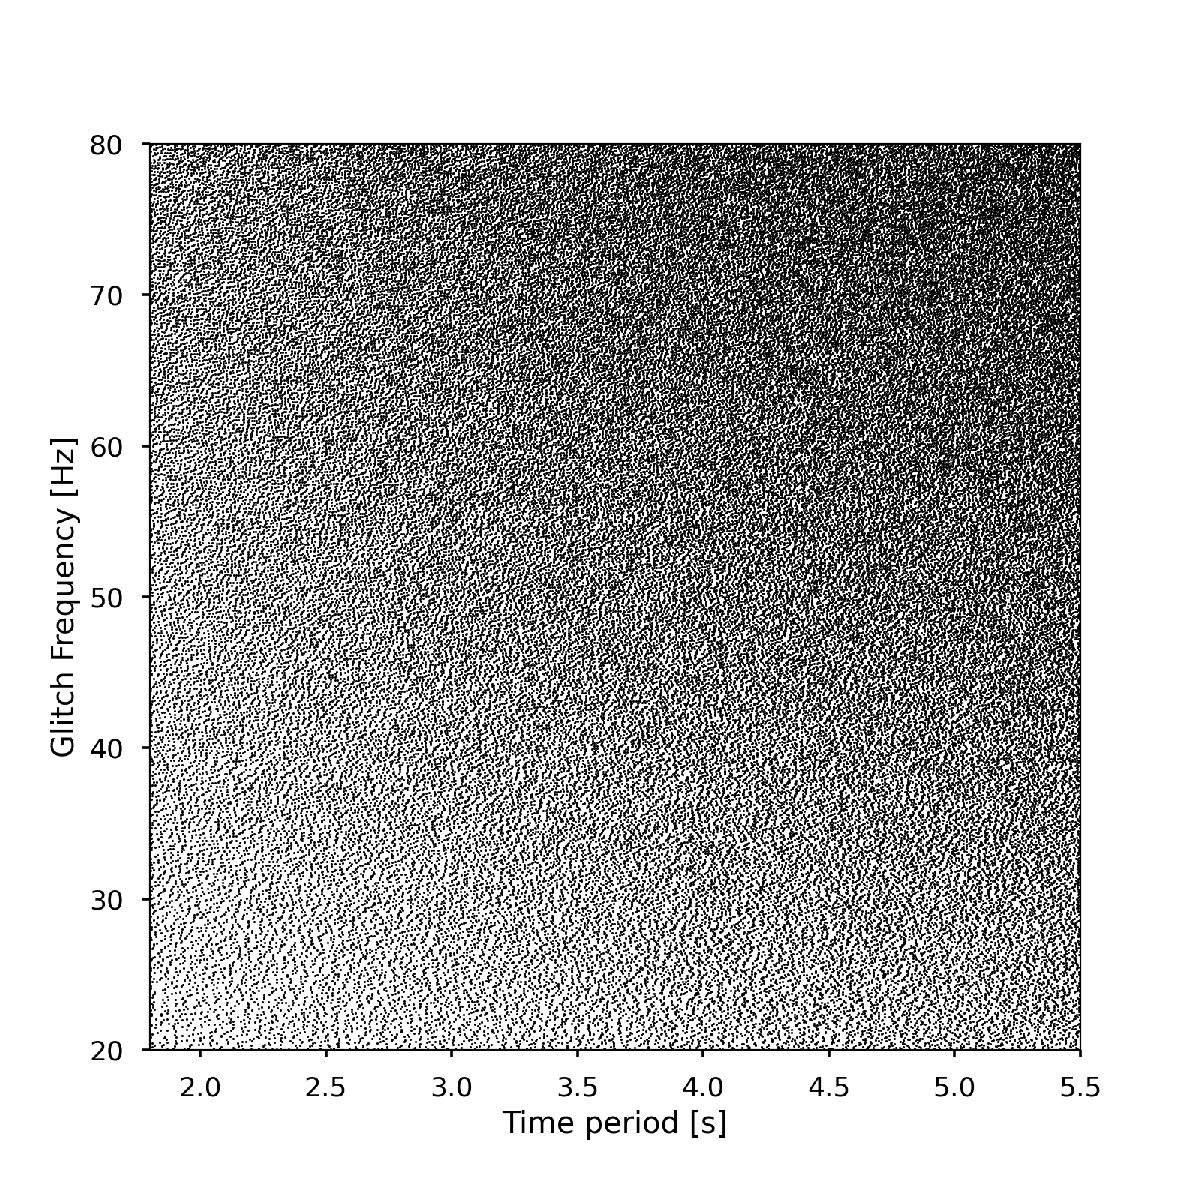
\includegraphics[width=0.7\textwidth]{Figures/Section3/3.2/template_bank_square.pdf}
  \caption{The template bank of \scl{} glitch templates (black points) used in the search for \scl{} glitches. The \emph{glitch frequency} parameter values range from $20$Hz - $80$Hz and the \emph{time period} parameter values range from $1.8$s - $5.5$s. This bank was created with a maximum match allowed between two templates of $0.97$ and contains 117,481 templates.}
  \label{fig:sq_bank}
\end{figure}

\subsection{Identifying potential \scl{} glitches in the data}

We test our method by searching through \gw{} data from 2019-11-18 16:13:05 - 2019-11-25 22:11:09 for the LIGO-Hanford and LIGO-Livingston detectors. This time corresponds to the 25th period of data used in the LVK analysis of O3 data for compact binary mergers~\cite{gwtc3} and is prior to the implementation of RC tracking~\cite{reducing_scattering_o3} in these detectors. We only analyse data that is flagged as ``suitable for analysis" on the Gravitational Wave Open Science Center~\cite{GWOSC}\footnote{We note that in O3 \emph{only} data suitable for analysis is released, so we simply analyse all of the publicly available data.}. This corresponds to 5.96 days of analysable data for LIGO-Hanford and 5.93 days for LIGO-Livingston.

Equipped with our template bank we now identify potential \scl{} glitches in the data. We matched filter all of the data against all of the templates, producing a signal-to-noise ratio time series for every template in the bank. These signal-to-noise ratio time series will contain peaks which, when above a certain limit, indicate the presence of a \scl{} glitch at a particular time. We retain any maxima within the time series that have a signal-to-noise ratio greater than 8. However, as we do this independently for every template, we will identify multiple peaks for any given glitch, and we will also find peaks that correspond to other types of glitch, or even \gw{} signals. We discuss how we reduce this to a list of identified \scl{} glitches in the following subsections.

\subsection{Scattered-Light Signal Consistency Test}

To prevent the search for \scl{} glitches from misclassifying other classes of glitches, or \gw{} signals, we employ a $\chi^2$ consistency test. The $\chi^2$ discriminator introduced in \cite{Allen_2005} divides \gw{} templates into a number of independent frequency bins. These bins are constructed so as to contain an equal amount of the total signal-to-noise ratio (SNR) of the original matched filter between template and data. The $\chi^{2}$ value is obtained by calculating the SNR of each bin, subtracting this from the expected SNR value for each bin and squaring the output. These values are summed for all bins and this value forms the $\chi^{2}$ statistic,
%
\begin{equation}
  \chi_{r}^{2} = \frac{\chi^{2}}{\textrm{DOF}} = \frac{n}{2n - 2} \sum_{i=1}^n \left(\frac{\rho}{\sqrt{n}} - \rho_{bin,i}\right)^2.
  \label{eqn:chi_squared}
\end{equation}
%
Here $n$ is the number of bins, $\rho$ is the SNR of the original matched filter between template and data, and $\rho_{bin}$ is the value of the SNR found when matched filtering one of the divided templates and the data. This test is constructed so as to produce large values when the data contains a glitch, or astrophysical signal, that is not well described by the template, but to follow a $\chi^2$ distribution if a glitch that matches well to the template is present, or if the data is Gaussian and stationary.

The $\chi^2$ test that we employ is similar to that of \cite{Allen_2005}, however compact binary merger waveforms increase in frequency over time whereas \scl{} glitch templates are symmetric about their centre. We therefore choose to construct our $\chi^2$ test with four non-overlapping bins \emph{in the time domain}, each of which contributes equally to the SNR, an example of the split template can be seen in figure \ref{fig:split_temp_subplot}. The matched filter between the bins and data is computed and the $\chi_{r}^{2}$ value is calculated using equation \ref{eqn:chi_squared} (where $n=4$). Any glitch, or astrophysical signal, which does not exhibit symmetric morphology should not fit with this deconstruction of the template, and should result in elevated $\chi_{r}^{2}$ values.

\begin{figure}
  \centering
  \begin{minipage}[t]{1.0\linewidth}
  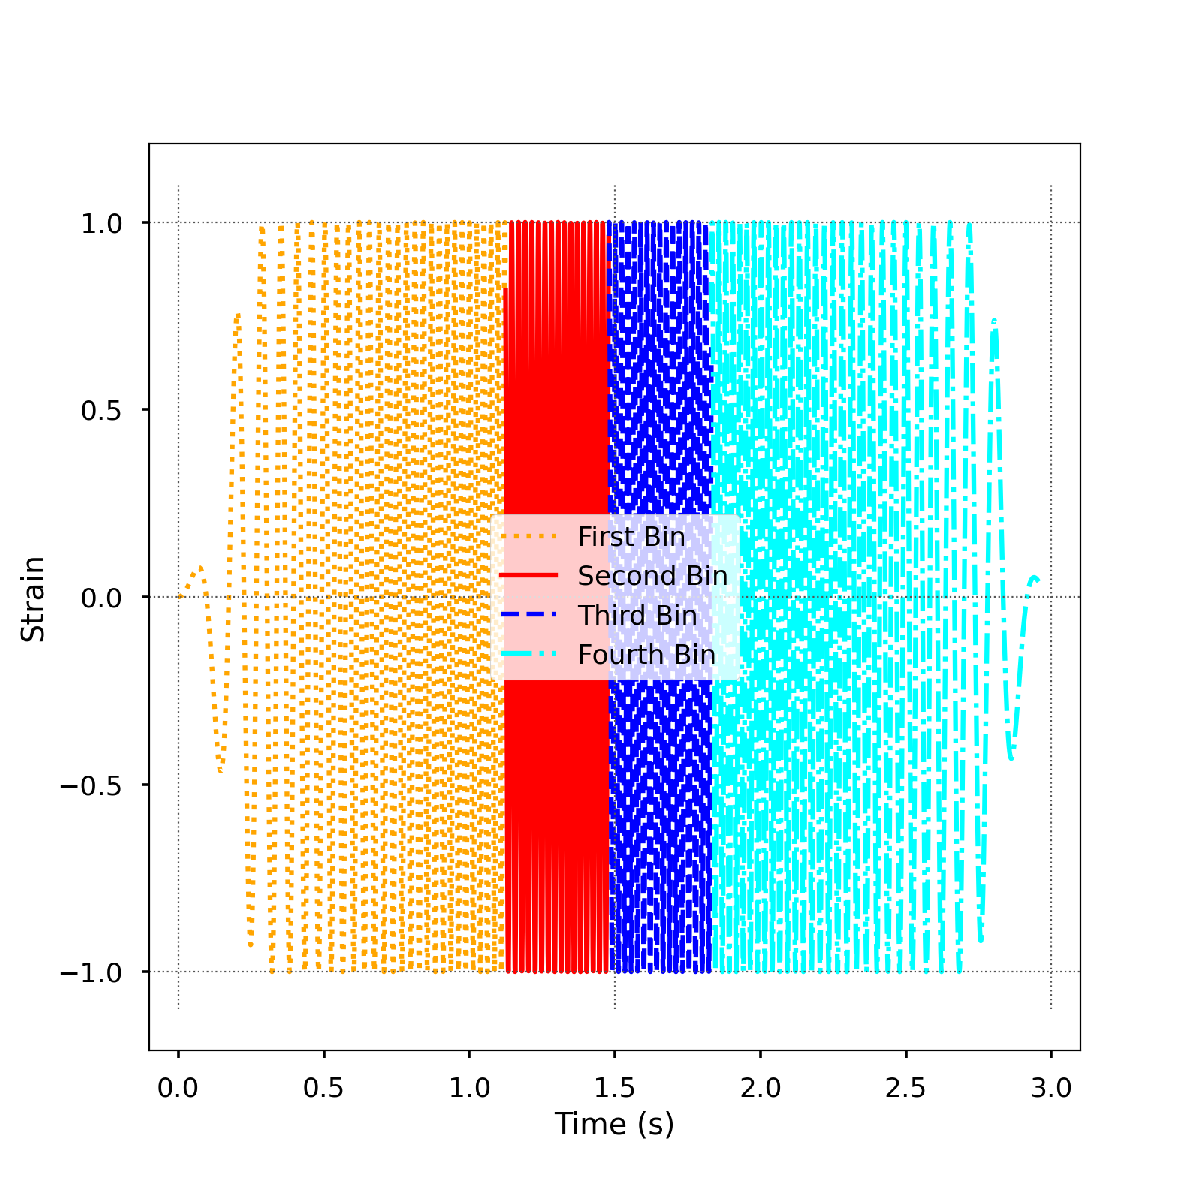
\includegraphics[width=0.49\textwidth]{Figures/Section3/3.4/split_bins.pdf}
  \hspace{0.01\linewidth}
  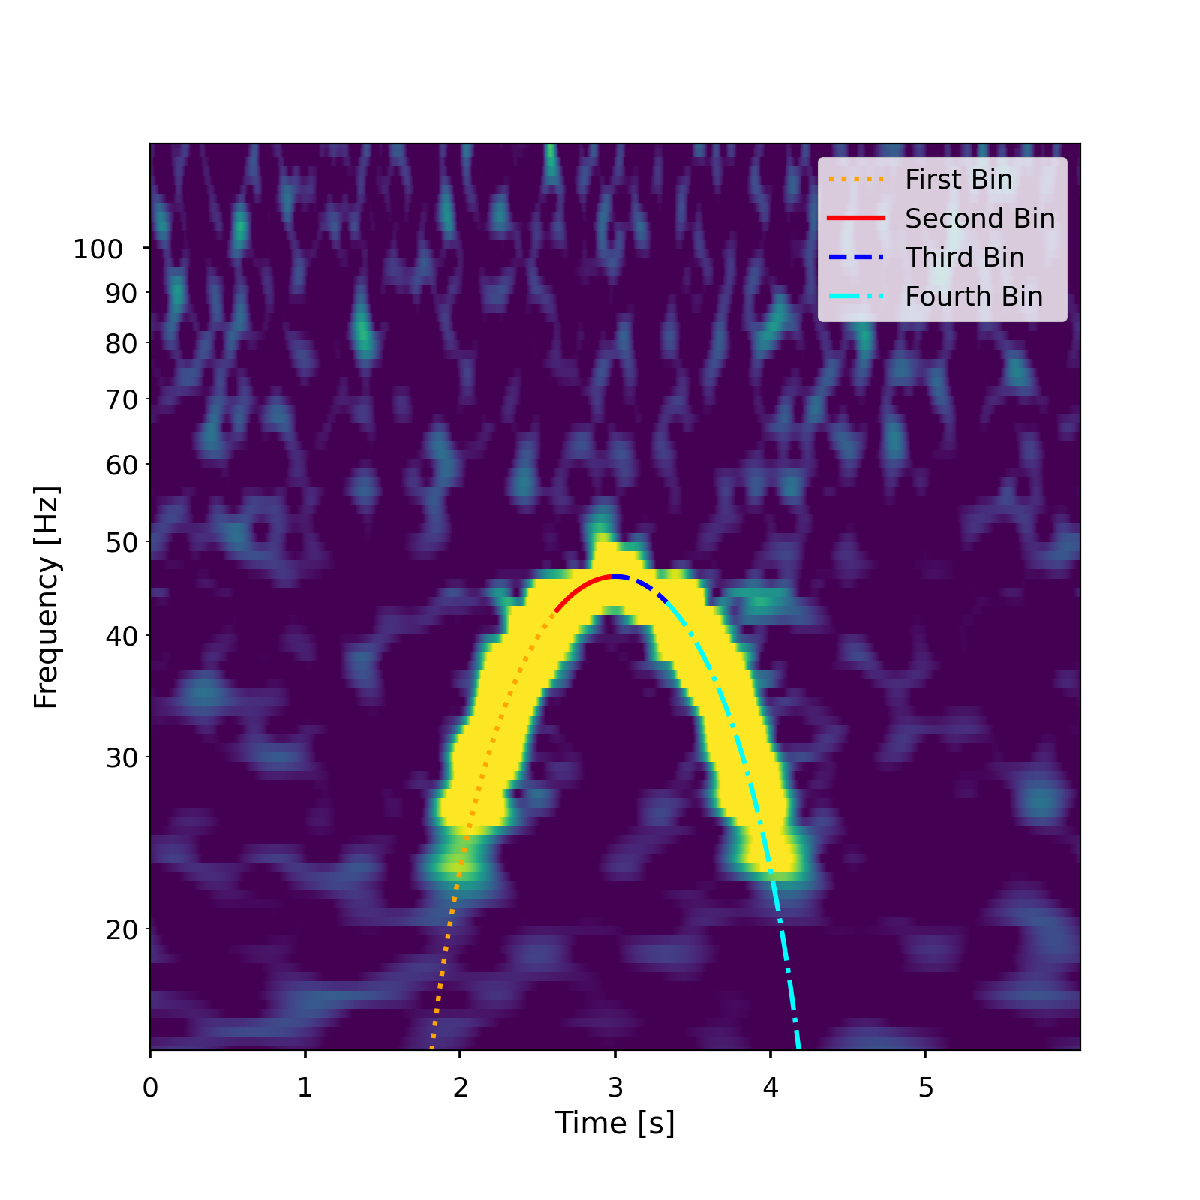
\includegraphics[width=0.49\linewidth]{Figures/Section3/3.4/split_bins_qscan.pdf}
  \end{minipage}
  \caption{A \scl{} glitch template (left) where the colours and line-styles are indicative of the four equal SNR time bins to be used in calculating the $\chi_{r}^{2}$ value and re-weighting the SNR. The same \scl{} glitch template bins overlaid on an injection of the \scl{} glitch (right). The inner two bins are considerably shorter than the outer two bins which informs us that the center - higher frequency - region of the \scl{} glitch contributes a larger amount to the SNR per unit time than the lower frequency regions.}
  \label{fig:split_temp_subplot}
\end{figure}

After computing the $\chi_{r}^{2}$ value for potential \scl{} glitches, we follow~\cite{rw_snr_eq} to compute a ``re-weighted signal-to-noise ratio'', which is an empirically tuned statistic depending on the signal-to-noise ratio and the $\chi_{r}^{2}$ value.  The re-weighting function we use matches that presented in~\cite{rw_snr_eq},
%
\begin{equation}
\rho_{rw} =  \left\{  \begin{array}{l@{\quad}cr} 
\rho & \mathrm{if} & \chi_{r}^{2} \leq 1, \\  
\rho [(1 + (\chi_{r}^{2})^3)/2]^{-\frac{1}{6}} &  \mathrm{if} & \chi_{r}^{2} \ge 1,   
\end{array}\right.
\label{eqn:reweighting}
\end{equation}
%
where $\rho_{rw}$ represents the re-weighted signal-to-noise ratio of the \scl{} glitch template calculated using the signal-to-noise ratio, $\rho$, and the $\chi_{r}^{2}$ value of that template.
We do note that this re-weighting function has been tuned for compact binary merger waveforms and we did not repeat that tuning here with \scl{} glitches. One could retune this statistic, specifically targeting \scl{} glitches, using (for example) the automatic tuning procedure described in~\cite{McIsaac_2022}. However, we demonstrate the suitability of the $\chi^{2}$ test for our purposes in figure~\ref{fig:chi_snr} where we show the $\chi_{r}^{2}$ vs SNR distribution of the triggers found by our \scl{} glitch search when performed on data containing only \scl{} glitches and data containing a binary black hole \gw{} injection.

\begin{figure}
  \makebox[\textwidth][c]{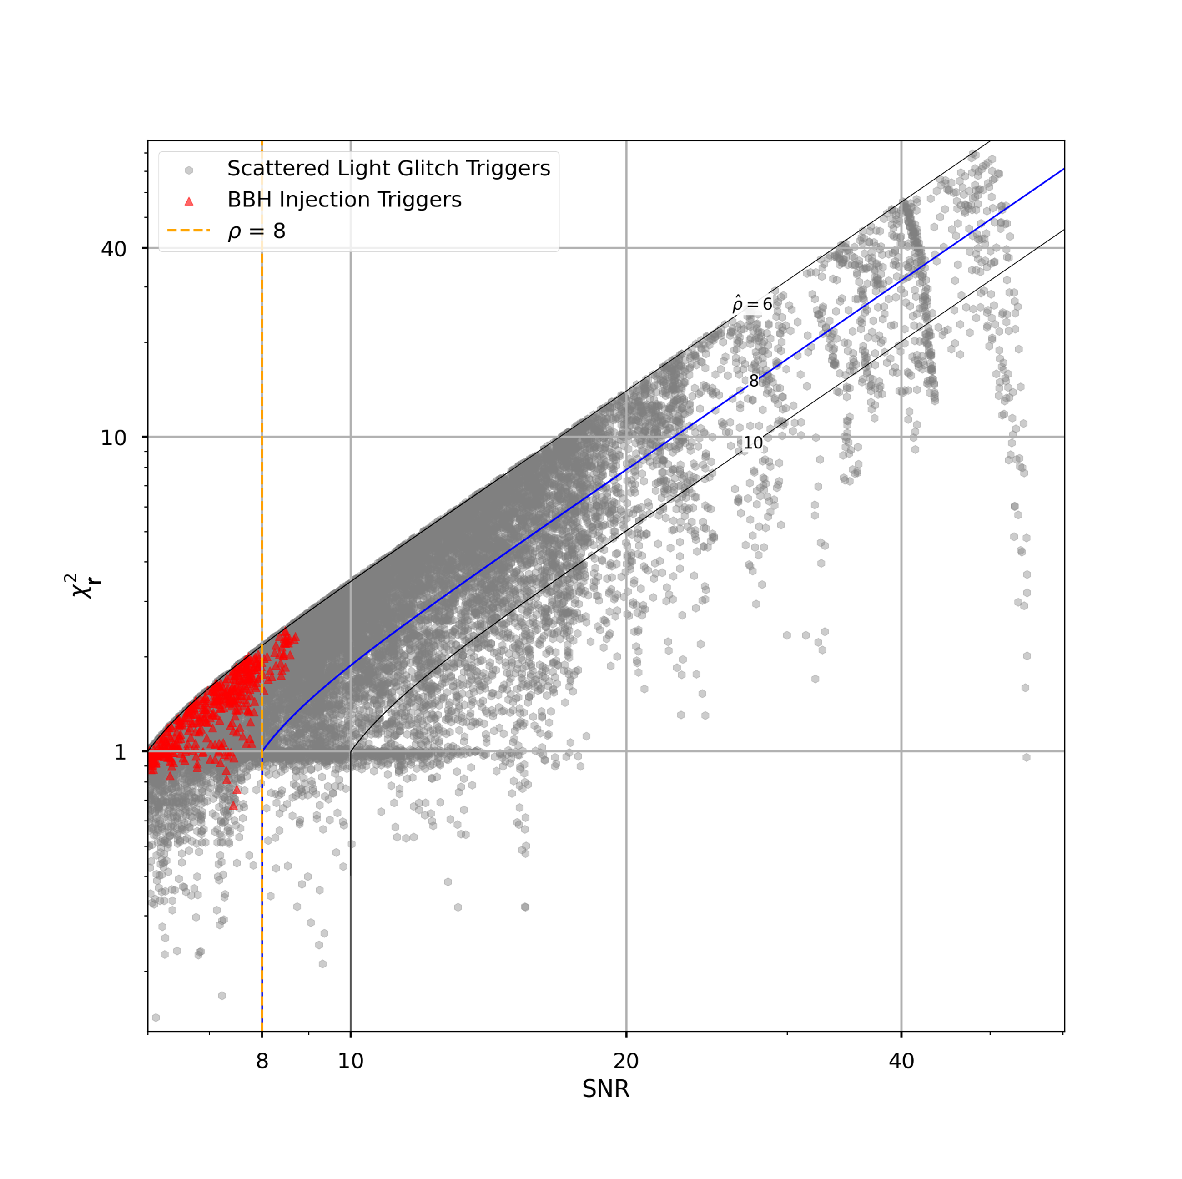
\includegraphics[width=\textwidth]{Figures/Section3/3.4/SLvsBBH.pdf}}
  \caption{The signal-to-noise ratio and $\chi_{r}^{2}$ values for the triggers identified by the matched filtering and clustering of the \scl{} glitch template bank with data containing only \scl{} glitches (grey hexagons) and data containing a binary black hole \gw{} injection (red triangles). The black contour lines represent the re-weighted signal-to-noise ratio values the trigger will take when equation \ref{eqn:reweighting} is applied. The orange dashed vertical line indicates the signal-to-noise ratio value limit of 8, above which we decide to perform the $\chi^{2}$ test and calculate the re-weighted signal-to-noise ratio. The blue solid contour line indicates a re-weighted signal-to-noise ratio value of 8, which is the limit at which we consider the trigger to be real. Different re-weighting parameter values will produce different contour line shapes. It can be seen that no triggers for the data containing the \gw{} injection lie beneath the contour line and therefore no \scl{} glitches are found on the \gw{} signal.}
  \label{fig:chi_snr}
\end{figure}

We note that the $\chi^{2}$ test increases the number of matched filters required by the search and therefore the computational cost of the search. Each template would require the matched filtering of an additional $4$ ``binned'' templates to calculate the $\chi_{r}^{2}$ value to re-weight the SNR time series of that template, increasing computational cost by a maximum factor of $5$. However, we reduce this increase by only computing the $\chi^{2}$ where it is needed, specifically for any template where the SNR time series has values above the threshold of 8.

\subsection{Identifying all \scl{} glitches in the data}

\begin{figure}
      \begin{minipage}[t]{1.0\linewidth}
        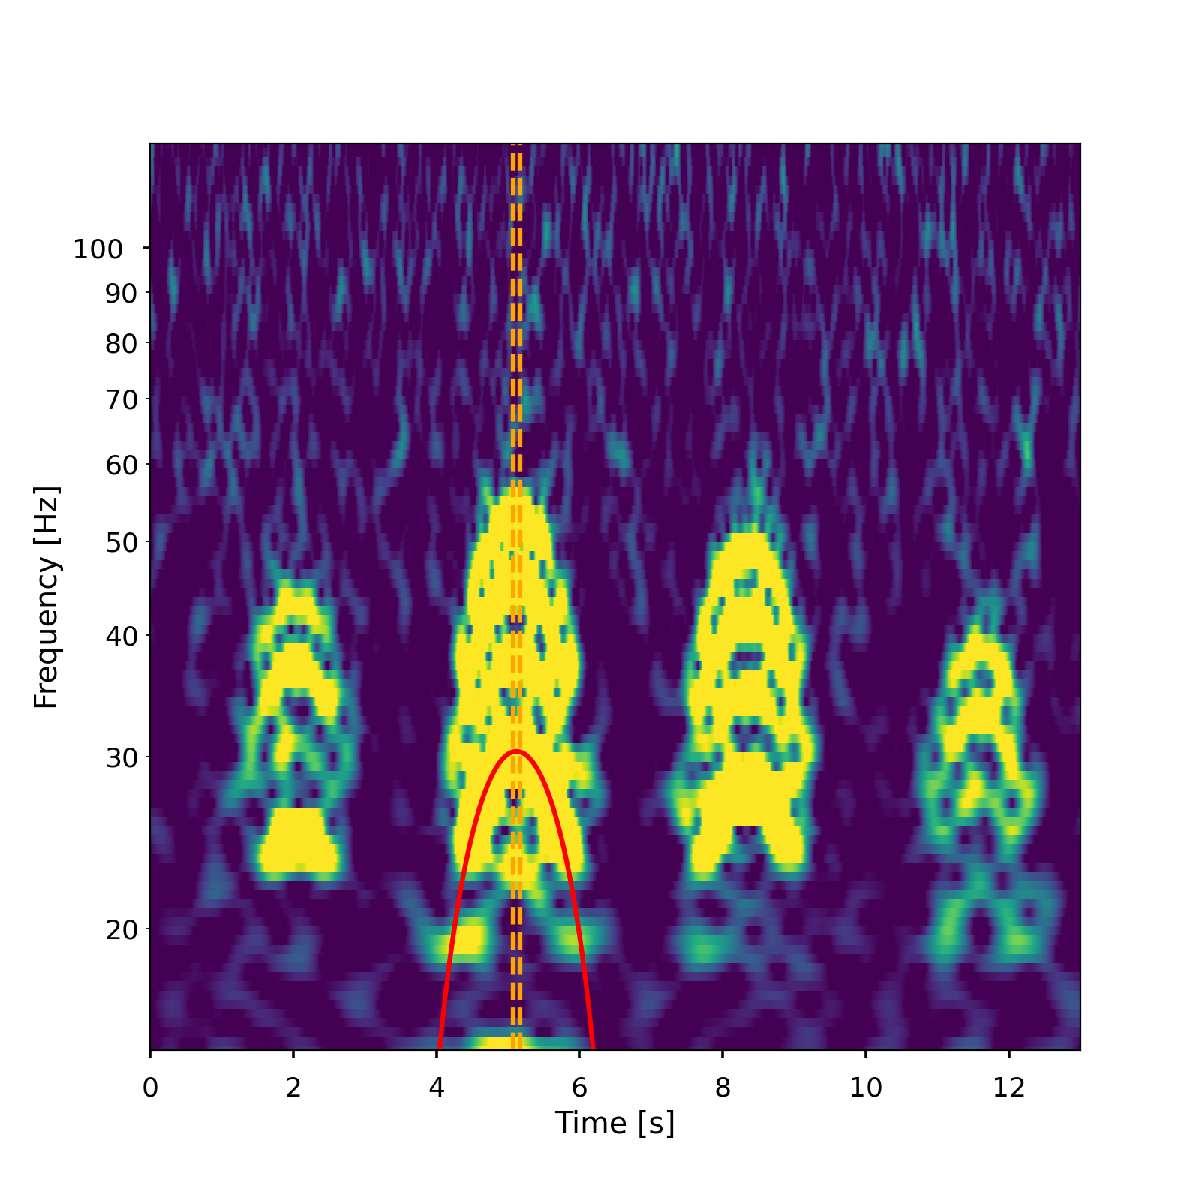
\includegraphics[width=0.49\linewidth]{Figures/Section3/3.5/cluster_qscan.pdf}
        \hspace{0.01\linewidth}
        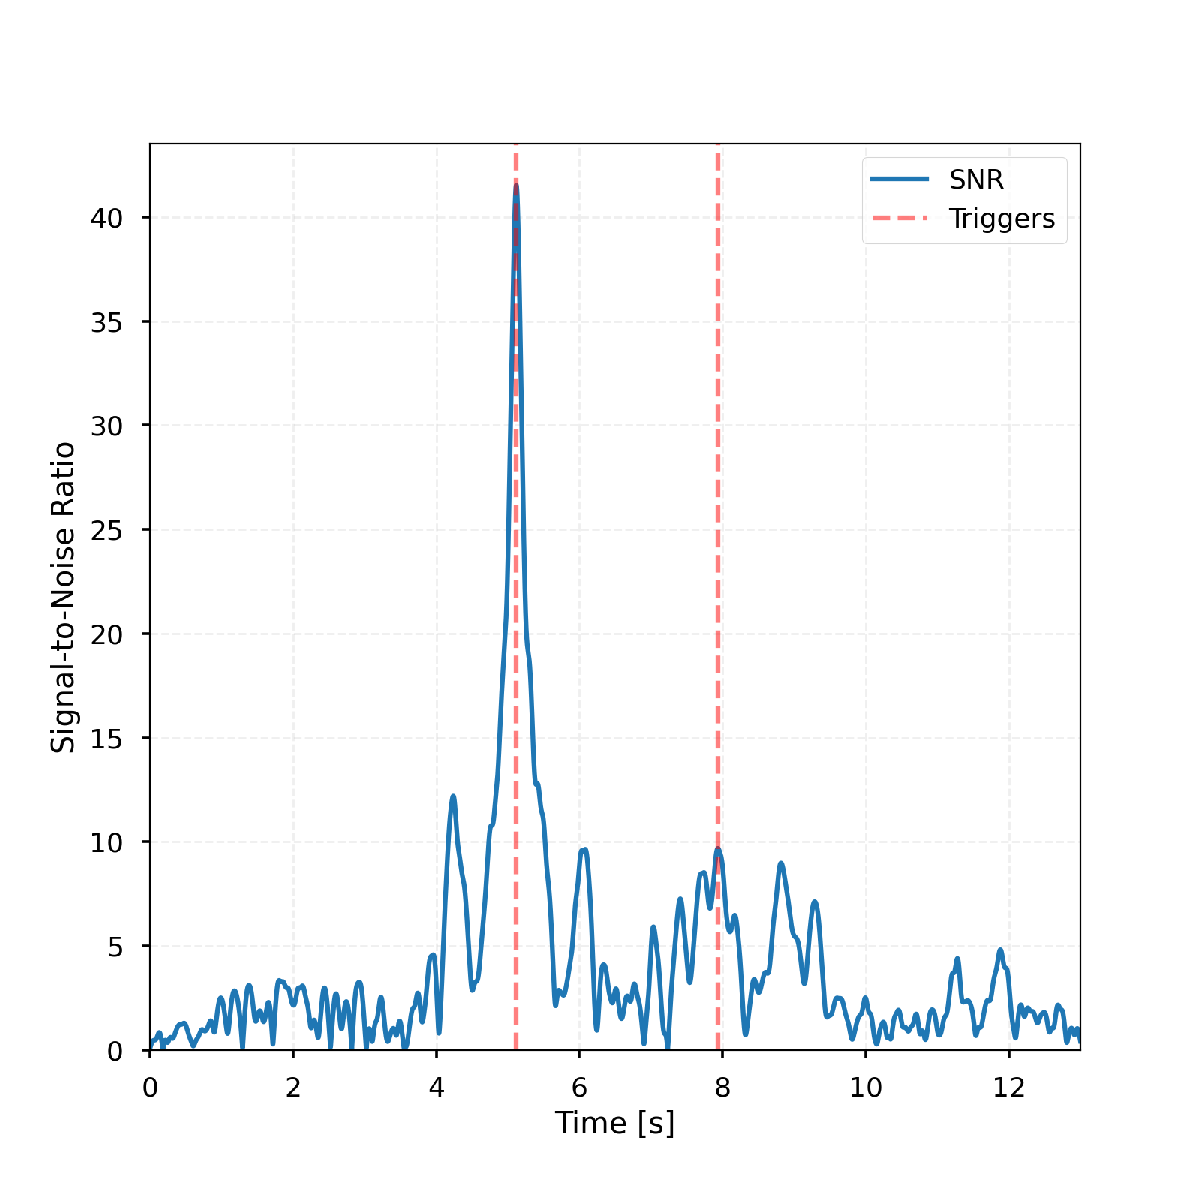
\includegraphics[width=0.49\linewidth]{Figures/Section3/3.5/cluster_snr_ts.pdf}
      \end{minipage}
      \begin{minipage}[t]{1.0\linewidth}
        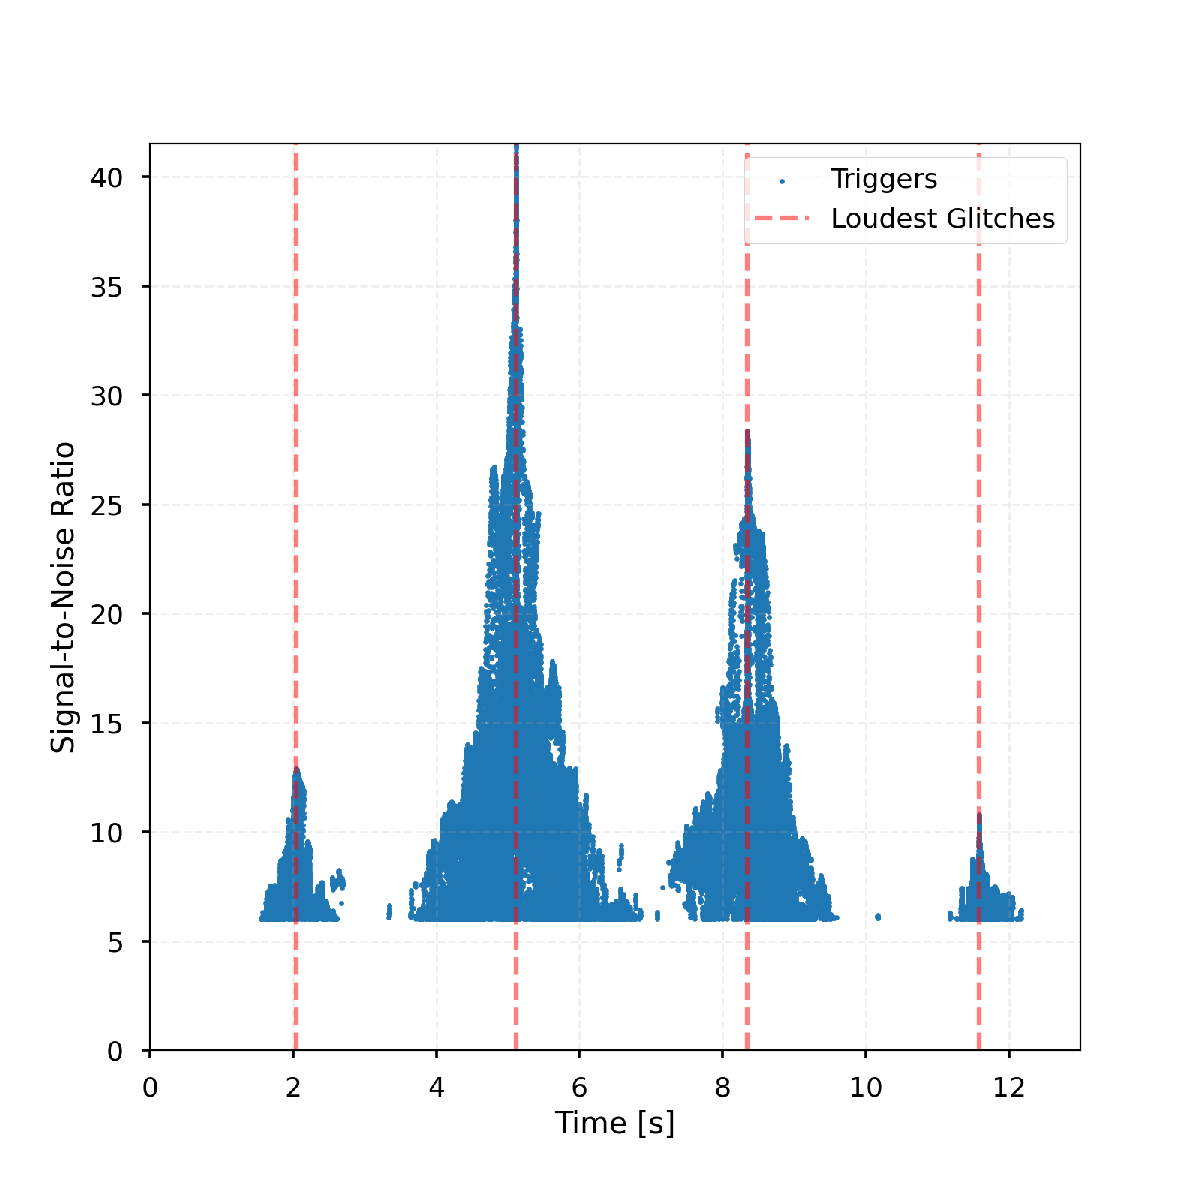
\includegraphics[width=0.49\linewidth]{Figures/Section3/3.5/cluster_all_triggers.pdf}
        \hspace{0.01\linewidth}
        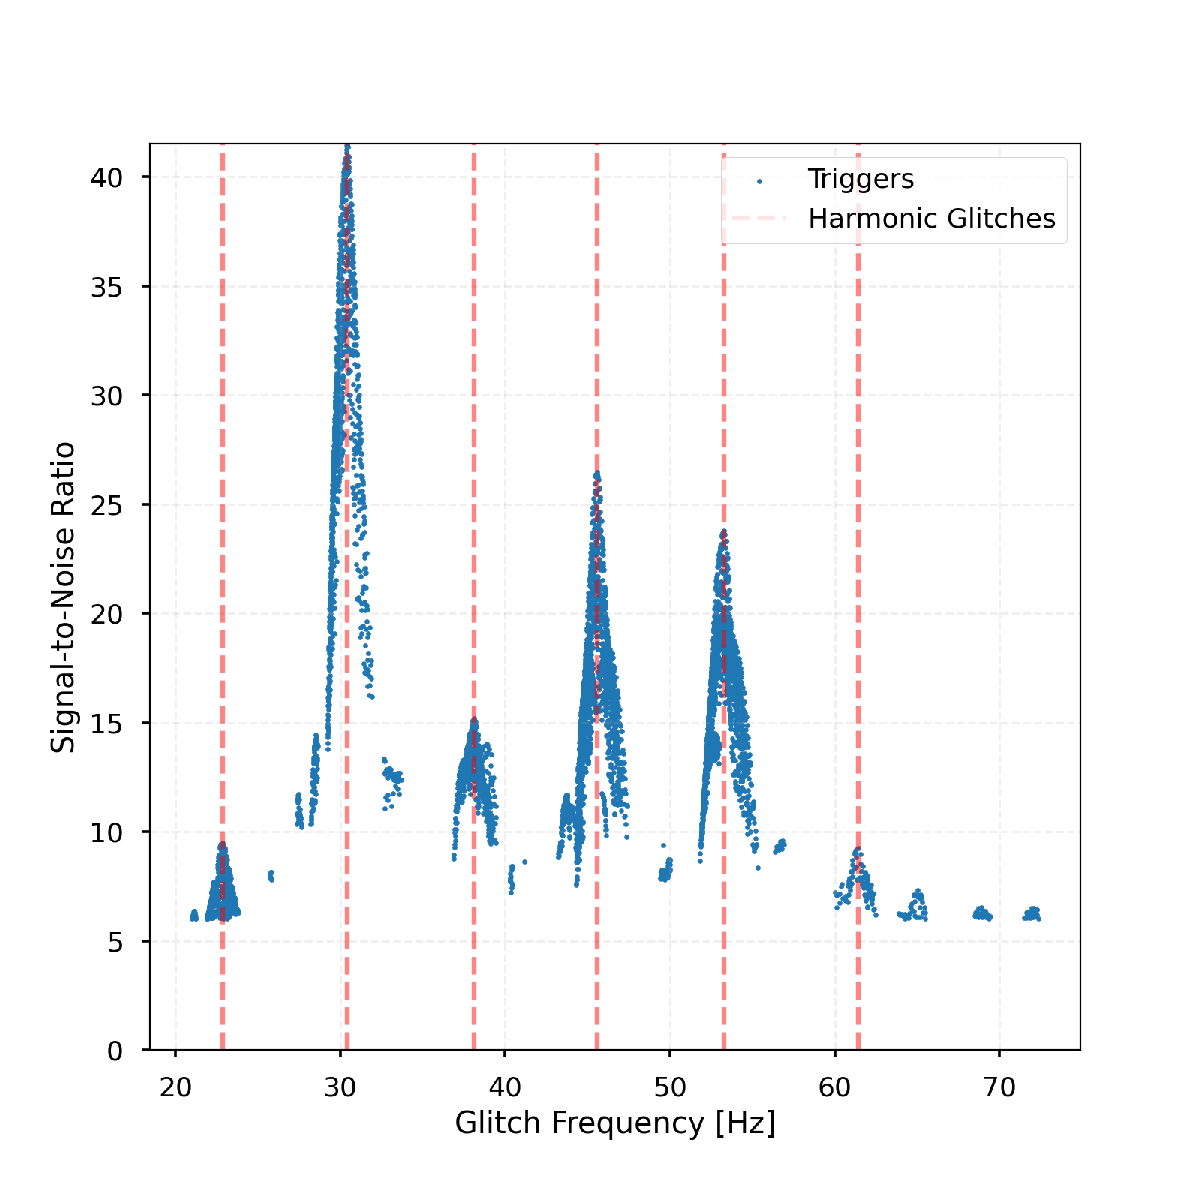
\includegraphics[width=0.49\linewidth]{Figures/Section3/3.5/cluster_in_frequency.pdf}
      \end{minipage}
    \caption{The process for identifying all the \scl{} glitches in a period of \gw{} data. The red overlay in the \gw{} data used in this example (top left) indicates the highest re-weighted signal-to-noise trigger found, the dashed vertical lines represent the time slice window around this trigger. The re-weighted signal-to-noise ratio time series resulting from the matched filter of this trigger's template and the data (top right) is clustered in time to identify the triggers found above a signal-to-noise threshold of $8$, indicated by red vertical dashed lines. All the triggers from all of the templates in the template bank are then clustered in time (bottom left) to identify the highest re-weighted signal-to-noise glitches in the data, indicated by the orange vertical dashes lines. The triggers found within the time slice window, with a similar \emph{time period} value---within $\pm 10\%$---of the highest re-weighted signal-to-noise ratio trigger (bottom right) are clustered by their \emph{glitch frequency} value to find the harmonic glitches at the same time, indicated again by red dashed lines.}
    \label{fig:clustering_story}
\end{figure}

Our matched filtering process retains ``triggers'' (potential \scl{} glitches) wherever the re-weighted signal-to-noise time series is larger than 8. We retain no more than one trigger within a window size equal to half the \emph{time period} of the template used to produce the re-weighted signal-to-noise time series and only store triggers at local maxima. A re-weighted signal-to-noise time series with multiple peaks and identified triggers can be seen in the top right panel in figure \ref{fig:clustering_story}.

After matched filtering all the templates against the data we will recover multiple triggers for any potential \scl{} glitch, as we might expect to independently identify peaks in multiple templates around the true values of the glitch. We therefore collect all of the triggers generated by the template bank and cluster these in time, using a window of half of the shortest duration template - $0.9$ seconds. This will result in a list of triggers corresponding to the highest re-weighted signal-to-noise ratios, where each trigger should correspond to a unique \scl{} glitch. The bottom left panel in figure \ref{fig:clustering_story} shows an example of the triggers found by the search and the highest re-weighted signal-to-noise ratio triggers found by clustering.

However, we also expect to see instances of harmonic glitches which are produced by the same scattering surface and so share the same \emph{time period} and have \emph{glitch frequency} values equal to a multiple of the lowest frequency glitch in the harmonic stack~\cite{TAccadia}. We investigate each trigger in the list, searching for harmonic glitches occurring at the same time. We use the first list of triggers identified by all templates across the bank and filter by those that occur within $\pm0.05$ seconds of the \emph{center time} of the trigger we are investigating, an example of this window can be seen in the top left panel of figure \ref{fig:clustering_story}. We then filter the triggers again, keeping only those with an associated \emph{time period} value within $\pm 10 \%$ of the trigger's \emph{time period}. Finally we cluster these remaining triggers by their associated \emph{glitch frequency} using a window size of $4$Hz, a lower limit on the frequency separation of harmonic glitches, the bottom right panel in figure \ref{fig:clustering_story} shows the identification of harmonic glitches for the overlaid \scl{} glitch in the top left panel of figure \ref{fig:clustering_story}.

\subsection{Hierarchical subtraction to find parameter values}

We now have a list of identified \scl{} glitches and their parameter values, however, these might not be fully accurate when there are many glitches close in time and frequency, as illustrated in figure~\ref{fig:overlay_goods}. It is important that the parameters we find match well with the glitches in the data to remove as much power as possible.

To better identify the parameter values of the \scl{} glitches, we perform a hierarchical procedure using information about the glitches we have found so far. Firstly, we create new segments of time which we know contain \scl{} glitches, taking a window of $8$ seconds on either side of each previously identified glitch, if two glitch windows overlap they are combined into the same segment.

For each segment we then create a reduced template bank, consisting of templates ``close'' to the \scl{} glitches previously identified in the segment. We take the smallest and largest \emph{time period} and \emph{glitch frequency} glitches in the segment and bound the retained templates by these values with $\pm 0.25$ seconds on the \emph{time period} and $\pm 1$Hz on the \emph{glitch frequency}. For each data segment the reduced template bank is matched filtered with the data, the maximum re-weighted SNR value is found and the corresponding glitch is subtracted. We then matched filter \emph{again} and remove the next largest re-weighted SNR template. This process is repeated until no templates, when matched filtered with the data, produce any re-weighted SNR values above the SNR limit of $8$. This method of hierarchical subtraction produces our final list of \scl{} glitches.

A further benefit of using these shorter data segments is that we are estimating the PSD of the data using only a short period of data close to the \scl{} glitches being removed. This protects us from a rapidly changing PSD in non-stationary data, which might cause Gaussian noise to be identified with larger SNR in the periods where the PSD is larger. This can be resolved by including the variation in the power spectral density as an additional statistic in the re-ranking of triggers, which has been done for compact binary coalescence \gw{} searches in~\cite{Mozzon_2020}.

We demonstrate the hierarchical subtraction step on an amount of data which contains four injected \scl{} glitches in a single harmonic stack, this can be seen in figure \ref{fig:injected_glitches}. As shown, the \scl{} glitches are found and subtracted from the data leaving behind a cleaned segment of \gw{} data with no excess noise. Figure~\ref{fig:overlay_goods} shows the identified \scl{} glitch triggers before and after performing the hierarchical subtraction step on a stretch of data containing real \scl{} glitches. We identify more triggers prior to performing hierarchical subtraction, however there are more errant mismatches between \scl{} glitches and the overlaid templates. By performing the hierarchical subtraction, we more accurately identify \scl{} glitches, however, we miss some glitches that were previously identified. There is still some imperfection in this process and we do not refine the method further in this work, but highlight this as useful direction for future studies in removing \scl{} glitches. 

\begin{figure}
     \centering
     \begin{minipage}[t]{1.0\linewidth}
        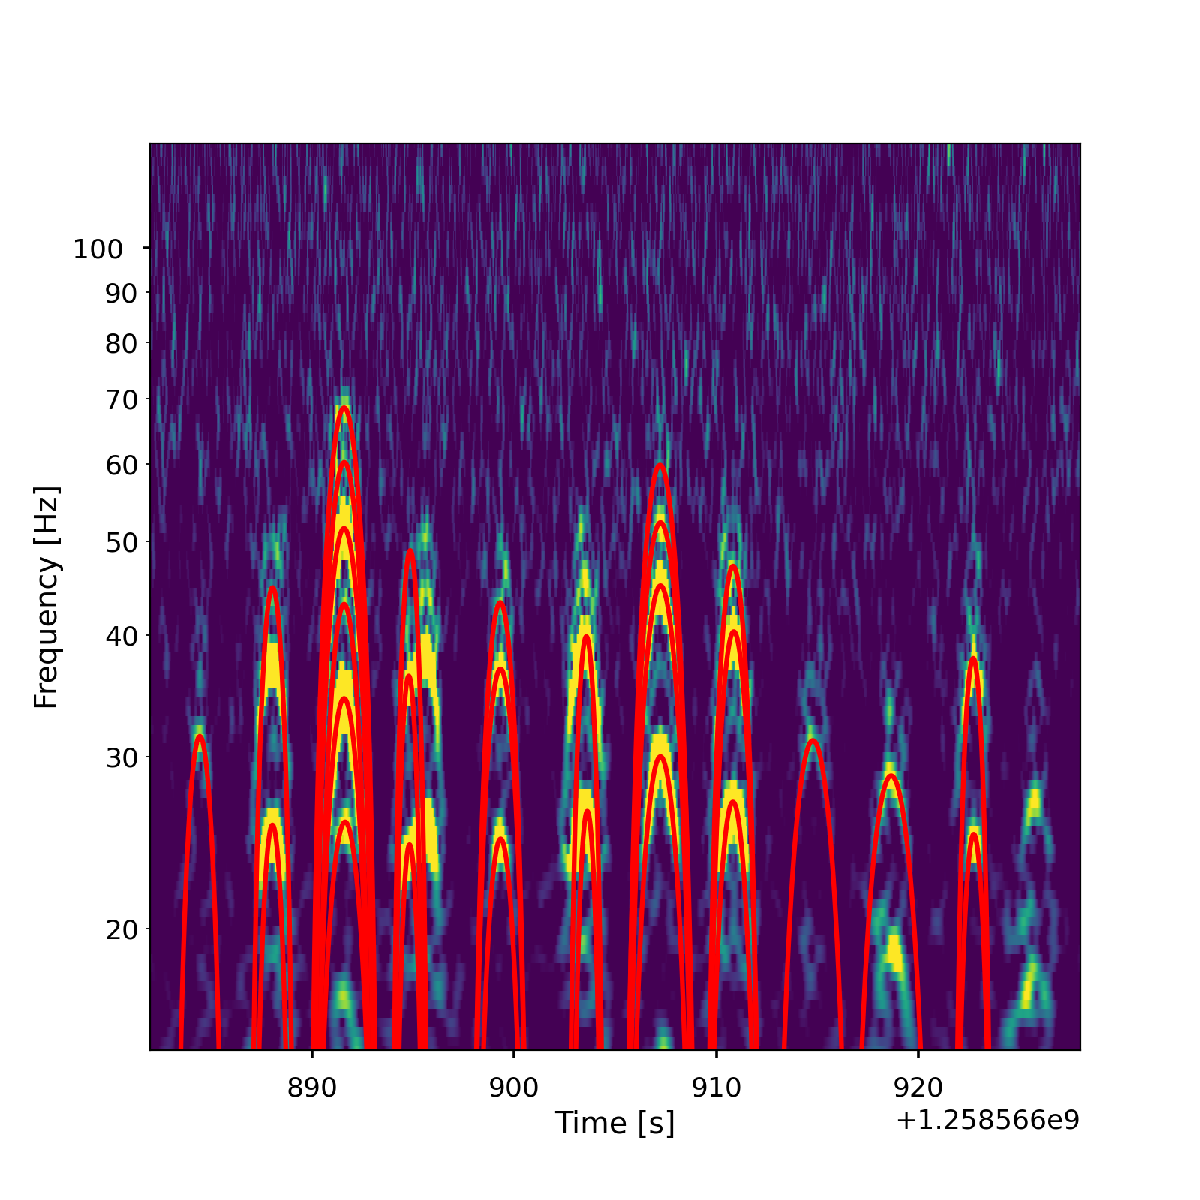
\includegraphics[width=0.49\linewidth]{Figures/Section3/3.6/overlay_good_overlays_first.pdf}
        \hspace{0.02\linewidth}
        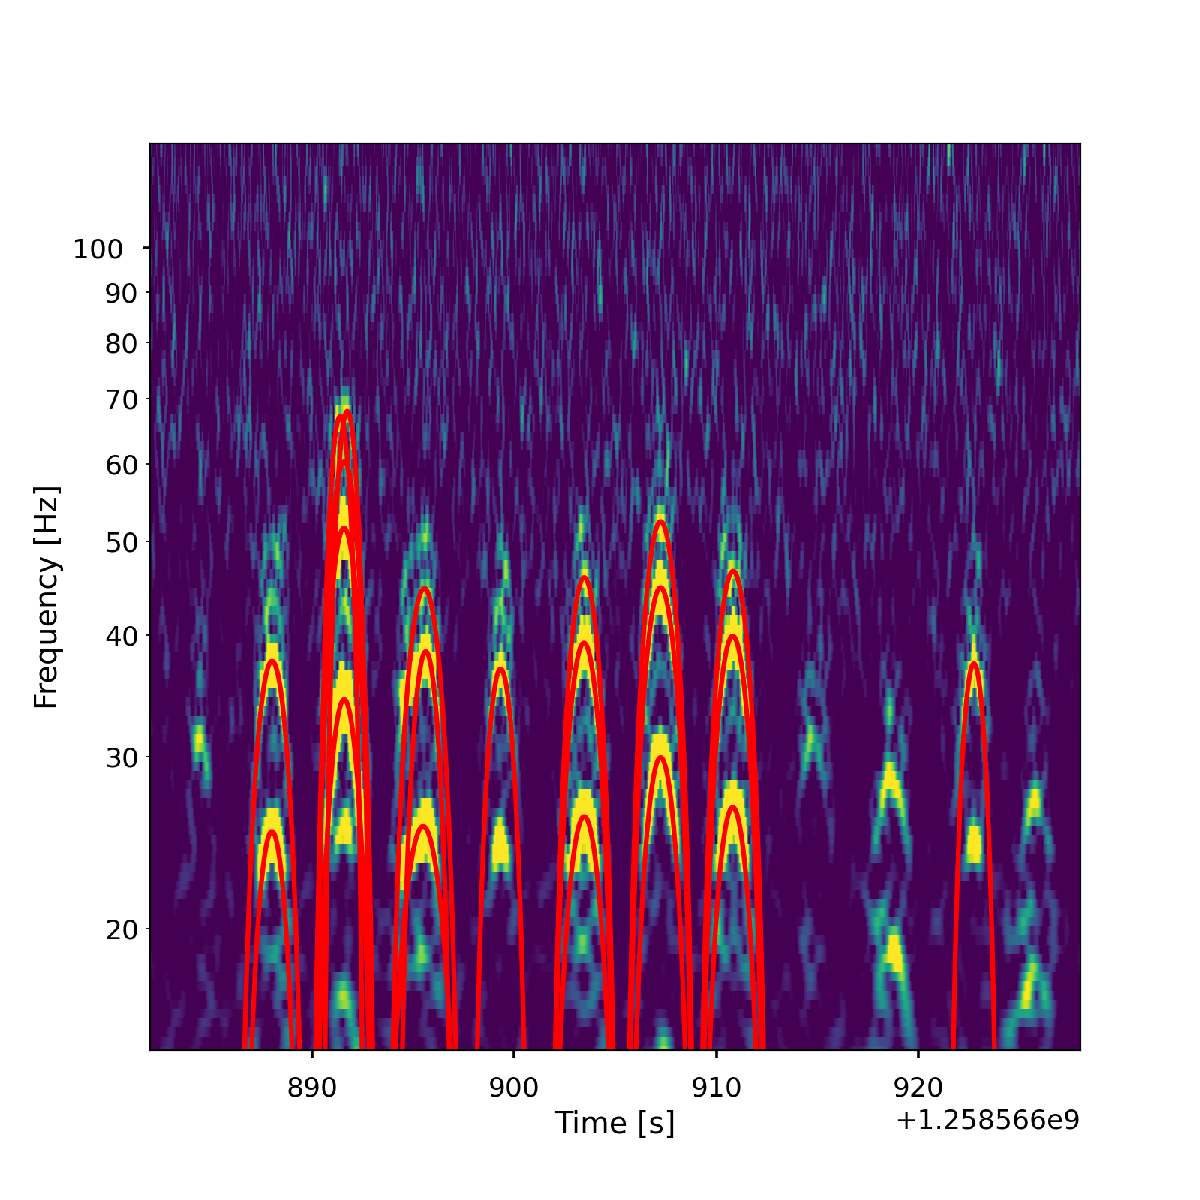
\includegraphics[width=0.49\linewidth]{Figures/Section3/3.6/overlay_good_overlays_second.pdf}
     \end{minipage}
         \caption{LIGO-Hanford data from 2019-11-23 17:54:22 - 2019-11-23 17:55:12 containing \scl{} glitches which have been identified by the ArchEnemy search (left), there is a misalignment in the template found for a number of glitches in this period of data and some missed glitches. \Scl{} glitches remaining after running the hierarchical subtraction search (right) for the same period of data, we have missed more \scl{} glitches however misalignments have been removed. The highest harmonic at approximately $892$ seconds has been incorrectly split into two separate templates.}
    \label{fig:overlay_goods}
\end{figure}

\begin{figure}
     \centering
     \begin{minipage}[t]{1.0\linewidth}
        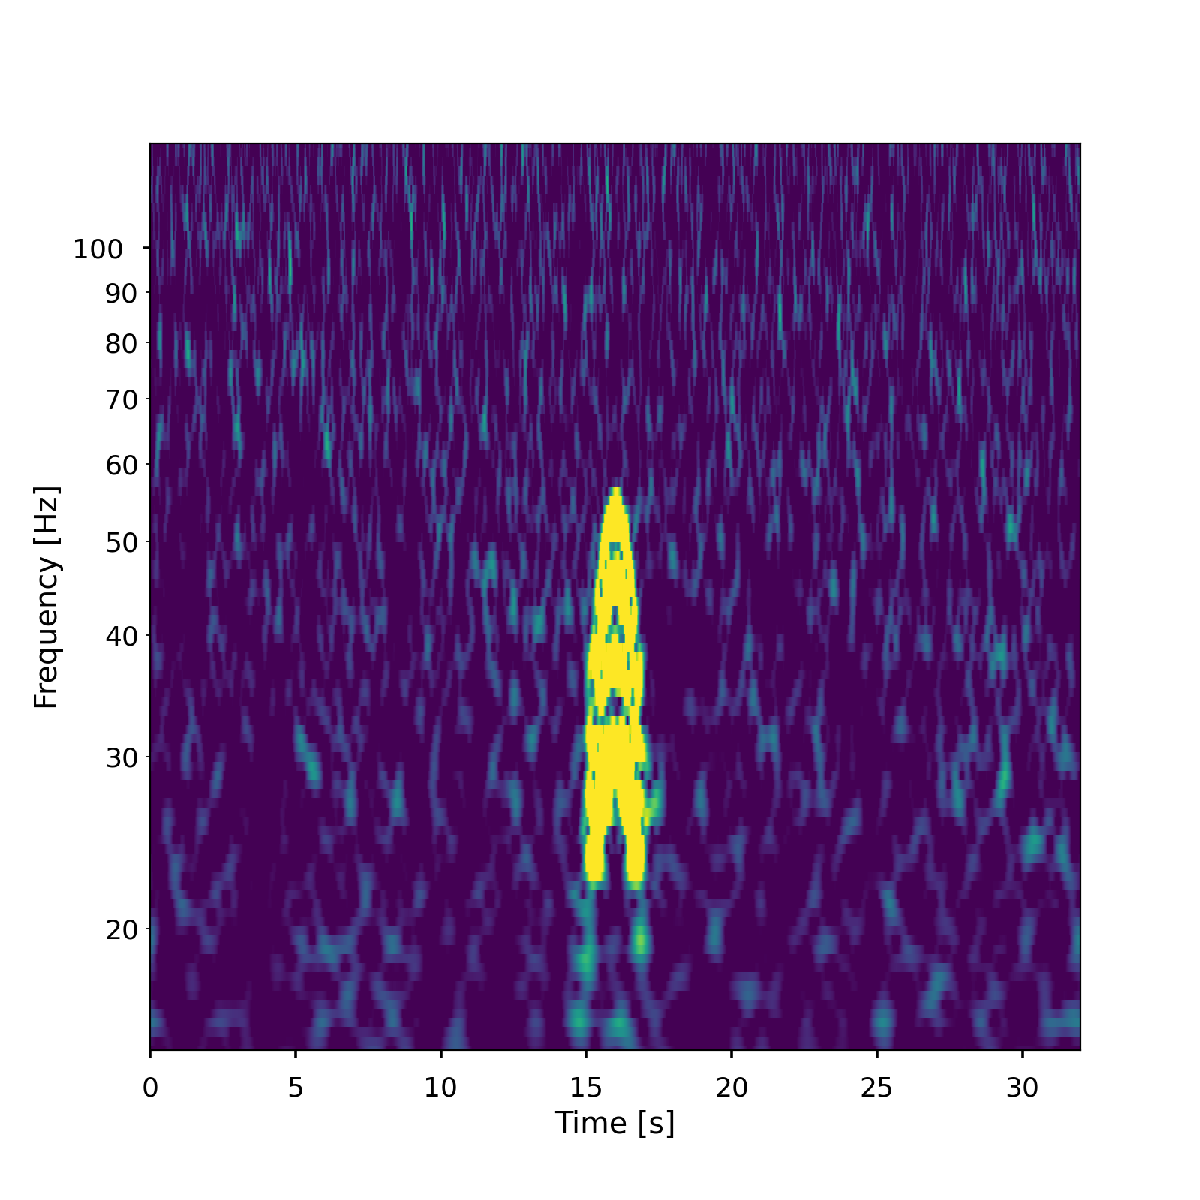
\includegraphics[width=0.49\linewidth]{Figures/Section3/3.6/injected_artefacts_initial.pdf}
        \hspace{0.02\linewidth}
        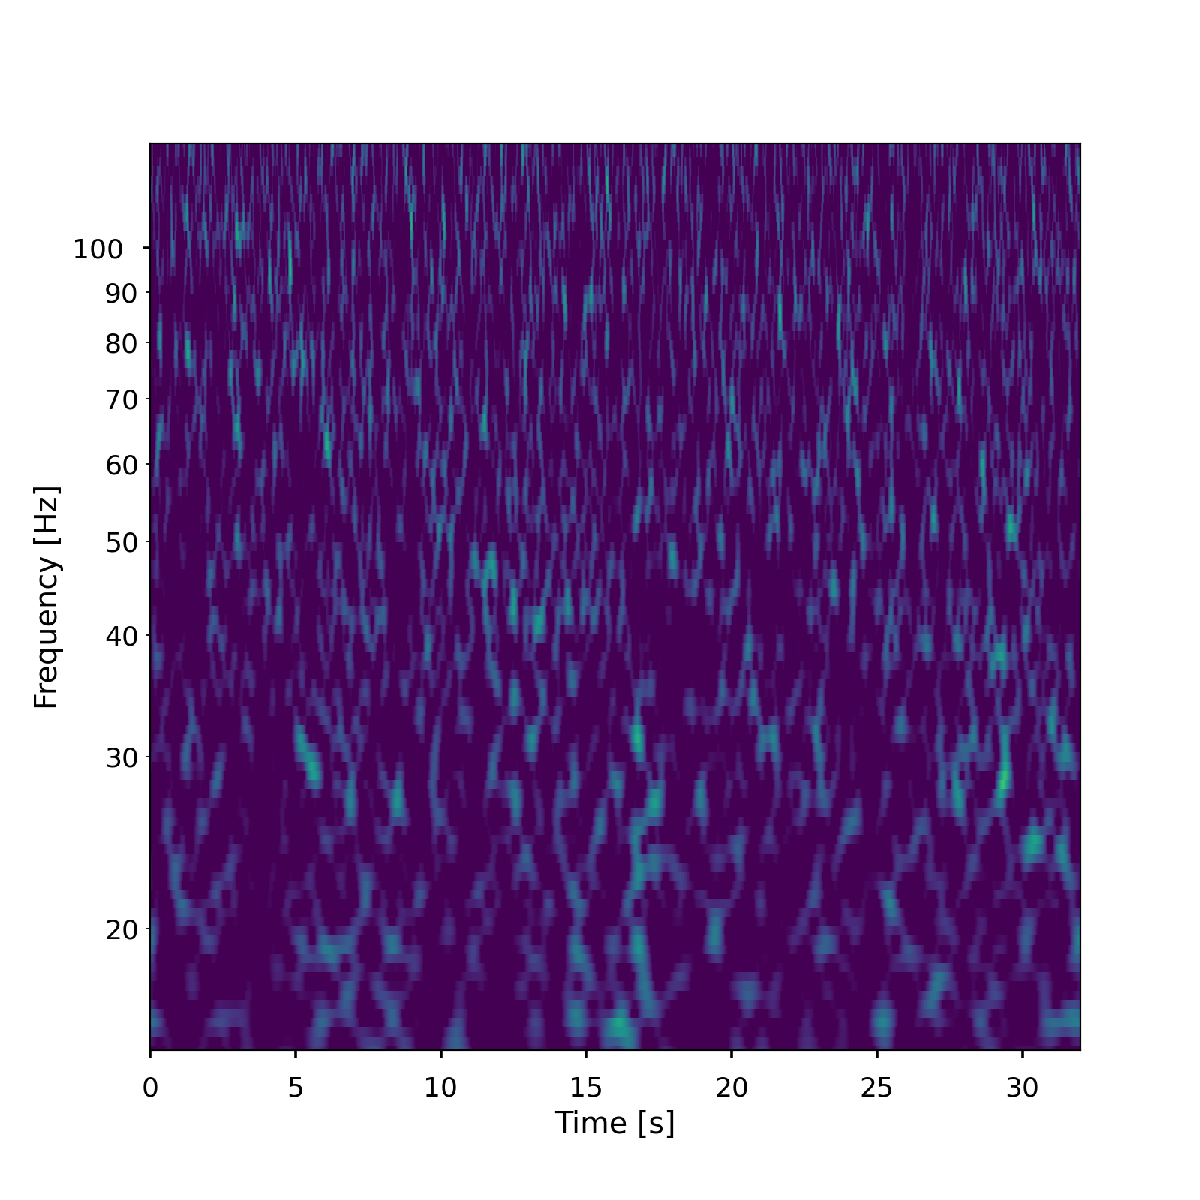
\includegraphics[width=0.49\linewidth]{Figures/Section3/3.6/injected_artefacts_subtracted.pdf}
     \end{minipage}
         \caption{Data containing an injected stack of harmonic \scl{} glitches (left) and the corresponding data found when running the hierarchical subtraction search and subtracting the identified \scl{} glitches from the data (right).}
    \label{fig:injected_glitches}
\end{figure}

\subsection{Identified \scl{} glitches}

The methodology described in previous sections is implemented in our ``ArchEnemy'' pipeline, which is capable of searching for \scl{} glitches in \gw{} data using a pre-generated bank of glitch templates. We use ArchEnemy to analyse the aforementioned data, which produced a list of $2749$ \scl{} glitches in data from the LIGO-Hanford observatory and $1306$ from the LIGO-Livingston observatory.

The number of \scl{} glitches found by the ArchEnemy pipeline can be compared to Gravity Spy for the same period of time. Gravity Spy finds $2731$ and $1396$ for LIGO-Hanford and LIGO-Livingston respectively~\cite{gravityspy}. There will be a difference in the number of glitches found by ArchEnemy and Gravity Spy for at least two reasons: Gravity Spy treats an entire stack of harmonic glitches as a single \scl{} glitch whereas ArchEnemy will identify each glitch as a separate occurrence. Gravity Spy can also identify \scl{} glitches which are not symmetric and fall outside our template bank, for example, the \scl{} glitches shown in figure~\ref{fig:overlay_bads}.

Figure~\ref{fig:overlay_goods} is an example of the results of the ArchEnemy pipeline and how well it has identified \scl{} glitches in a period of data. A majority of the glitches have been identified with the correct parameter values and even in cases where the chosen template is not visually perfect, there is a good match between the template and the identified power in the data, particularly in the case of slightly asymmetric glitches. Figure~\ref{fig:overlay_bads} demonstrates a period of time where the ArchEnemy pipeline has not fitted well the \scl{} glitches in the data. The glitches at this time are improperly fit by the templates due to asymmetry of the morphology of the glitches and because some of the glitches are outside of our template bank parameter range. However, we note that this is a very extreme period of \scl{} glitching and immediately after this time the detector data is no longer flagged as ``suitable for analysis''.

\begin{figure}
       \centering
    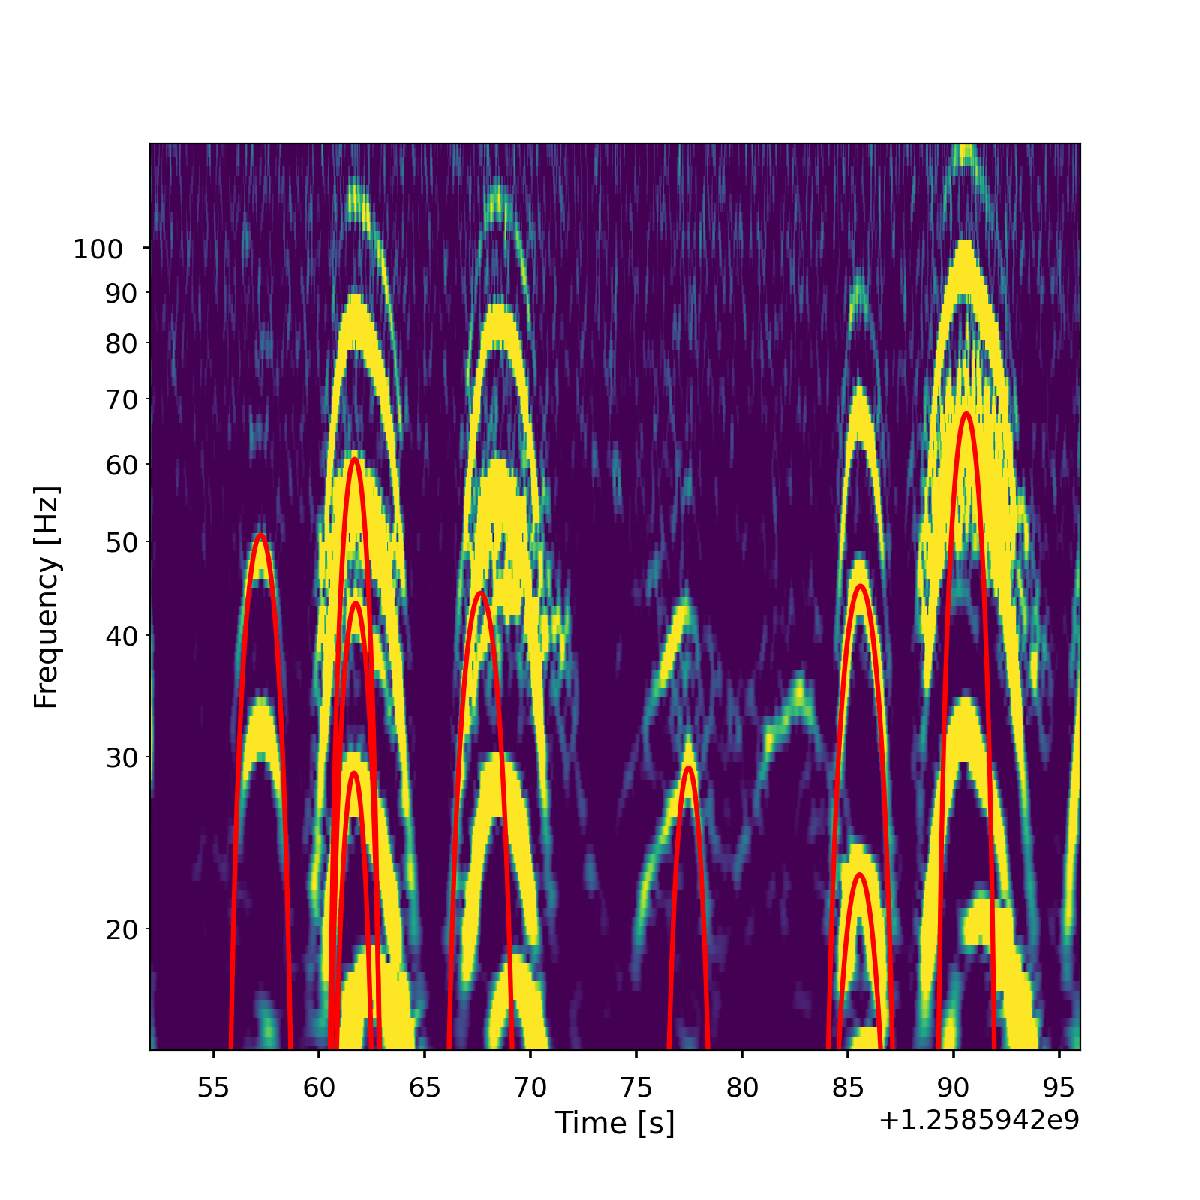
\includegraphics[width=0.7\linewidth]{Figures/Section3/3.7/overlay_bad_overlays.pdf}
    \caption{LIGO-Livingston data from 2019-11-24 01:30:32 - 2019-11-24 01:31:20 containing a very large number of \scl{} glitches at multiple times and frequencies over-plotted with the \scl{} glitches identified by the ArchEnemy search. Very few overlays match well onto \scl{} glitches. The template bank used in this search terminates at $80$ Hz and so the \scl{} glitches located above this value will not be correctly identified. There are also asymmetric \scl{} glitches located which will not be identified correctly by our search which assumes symmetry in the \scl{} glitch.}
    \label{fig:overlay_bads}
\end{figure}

We have demonstrated the ArchEnemy pipeline on a stretch of data from O3 and have identified and characterized a list of \scl{} glitches, which could be removed from the data. We do note that there are cases where the identification has not worked well, but we expect that subtracting our list of glitches from the data will reduce their effect on the \gw{} search. In the next section we will demonstrate this by quantifying sensitivity with the PyCBC pipeline.

\subsection{Safety of \scl{} identification}
\label{ssec:injsafety}

The data we have searched through contains no previously identified \gw{} signals~\cite{gwtc3}. However, there is a risk that the ArchEnemy search would identify real \gw{} signals as \scl{} glitches. To assess this possibility we simulate and add a large number of \gw{} signals into the data and assess whether any signals are misidentified.

To do this, we use three separate sets of simulated \gw{} signals (or ``injection sets''), one for BBHs, another for binary neutron stars (BNSs) and a third for neutron star black hole (NSBH) systems. We use the same simulations as the LVK search of this data, detailed in the appendix of~\cite{gwtc3}. Each injection set consists of $6200$ simulated signals spaced between $82$ and $120$ seconds apart. We treat these injection sets exactly the same as for the injection-less data, adding the simulations to the data, and then running ArchEnemy to produce a list of \scl{} glitches for each injection set.

To determine whether we have misidentified any \gw{} injections as \scl{} glitches we look for glitches we have found within the overlapping frequency band of \gw{} signals and our \scl{} glitch template bank. This corresponds to approximately $15$ second before merger time for the injections. The simulated signals occur every $\sim100$ seconds so we expect to see glitches within this $15$ second window, therefore, we also require that there must be more triggers identified in the \scl{} glitch search \emph{with} injections when compared to the search \emph{without} injections within the window. The details of the number of \gw{} injections with overlapping \scl{} triggers can be seen in table~\ref{tab:coincident_triggers}.

\begin{table}[tb]
\caption{\label{tab:coincident_triggers}For both interferometers and all $3$ injection sets we identify the number of injections which are found to have \scl{} glitches identified within $15$ seconds of merger time (``Injections with Coincident Triggers''), along with the number of \scl{} glitches found within this window for these injections (``Scattered-Light Coincident Triggers''). We investigated each of these injections and recorded the number which actually had \scl{} glitches identified due to the injected \gw{} signal (``Actual Overlapped Injections'').}
\footnotesize
\begin{tabular}{ccccc}
\br
&    & Injections with& Scattered-Light & Actual Overlapped \\
Interferometer & Injection Set & Coincident Triggers& Coincident Triggers&Injections \\
\mr
H1 & BBH           & 20 & 45 & 1\\
   & BNS           & 23 & 50 & 2\\
   & NSBH          & 38 & 73 & 7\\
L1 & BBH           & 13 & 21 & 2\\
   & BNS           & 18 & 30 & 2\\
   & NSBH          & 35 & 56 & 16\\
\br
\end{tabular}

\end{table}

A \scl{} glitch will be identified close to a \gw{} signal in two cases: the ArchEnemy search is misidentifying the \gw{} signal as a glitch \emph{or} the simulated signal was added close to actual glitches and a change in the data has meant a different number of glitches has been identified. The presence of real \scl{} glitches means we might miss a \gw{} signal, therefore, we \emph{do} want to find and subtract glitches close to \gw{} signals, but we do not want to subtract power from the \gw{} signal itself. The \scl{} glitch $\chi^{2}$ test was designed to prevent the matching of \scl{} glitch templates on other causes of excess power, however, these results show it is not perfect.

We investigate each injection with coincident \scl{} triggers, seeing how many had misidentified \scl{} glitches on the inspiral of the \gw{} signal, this number can be seen in the column ``Actual Overlapped Injections'' in table~\ref{tab:coincident_triggers}. We have included an example of the matching of \scl{} glitches onto \gw{} injections in figure~\ref{fig:loud_inj}, the right panel shows the \gw{} data post glitch subtraction where it can be seen there is a portion of the power being subtracted from the signal. Although power is being removed from the signal, the \gw{} injection is still found by the search for \gws{}, which we will describe later. For the cases that we have investigated, we note that the behaviour shown in figure~\ref{fig:loud_inj} only happens for signals that have very large signal-to-noise ratio, and are therefore unphysically close to us. A similar effect is observed with the ``autogating'' process, described in~\cite{pycbc}, which prevents the detection of these loud signals. In contrast to the ``autogating'' though, signals like that illustrated in figure~\ref{fig:loud_inj} are still identified as \gw{} signals by the PyCBC search after \scl{} glitch removal.

\begin{figure}
  \centering
  \begin{minipage}[t]{1.0\linewidth}
    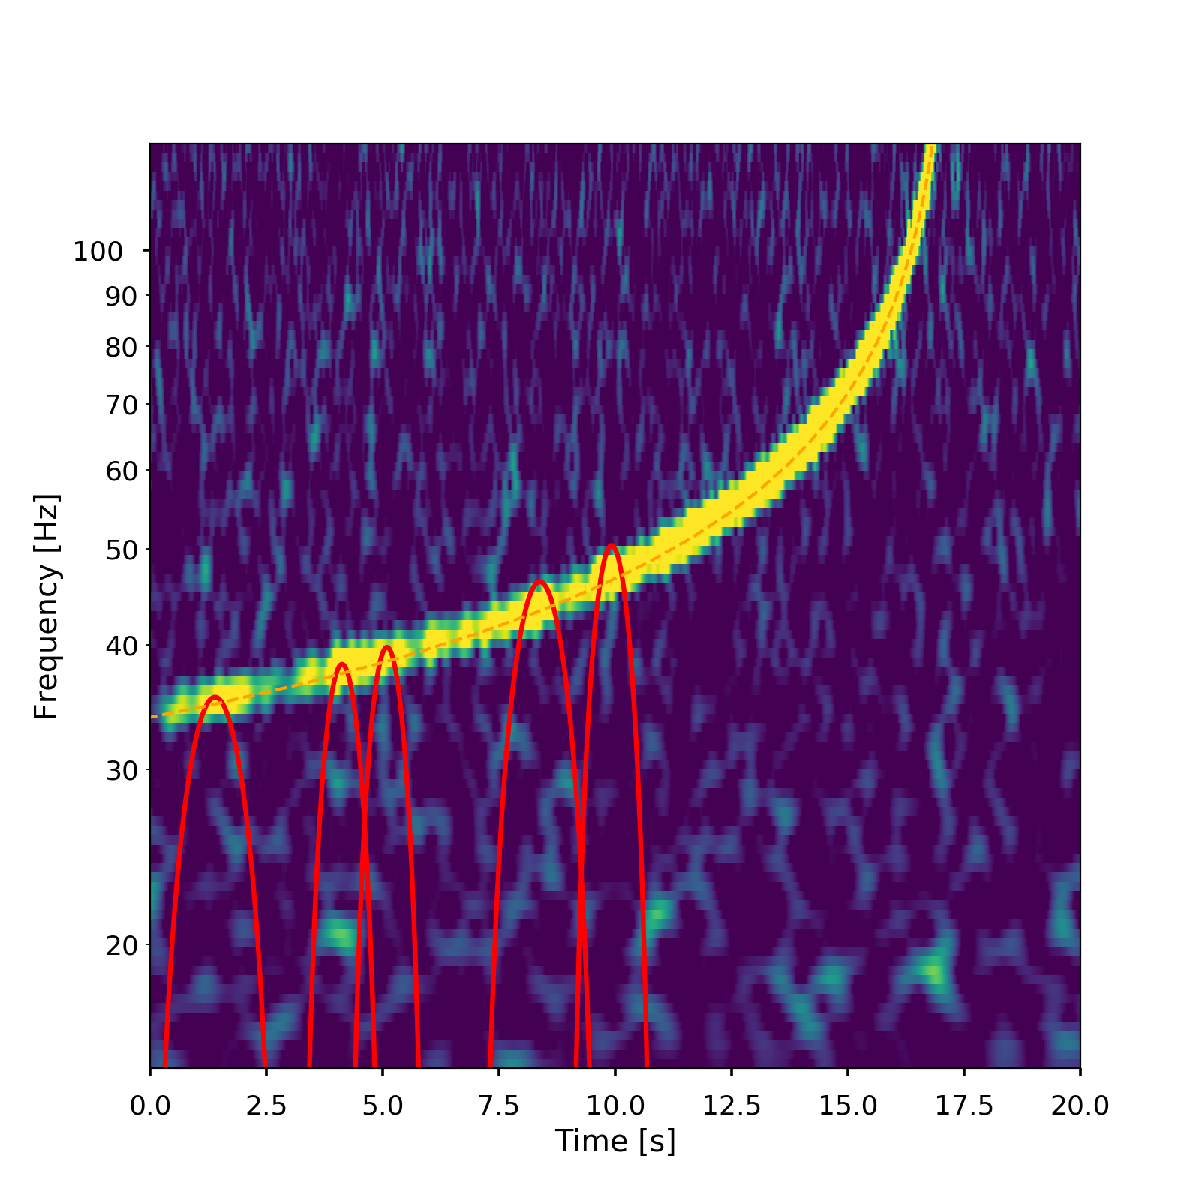
\includegraphics[width=0.49\linewidth]{Figures/Section3/3.8/L1_loud_Original.pdf}
    \hspace{0.02\linewidth}
    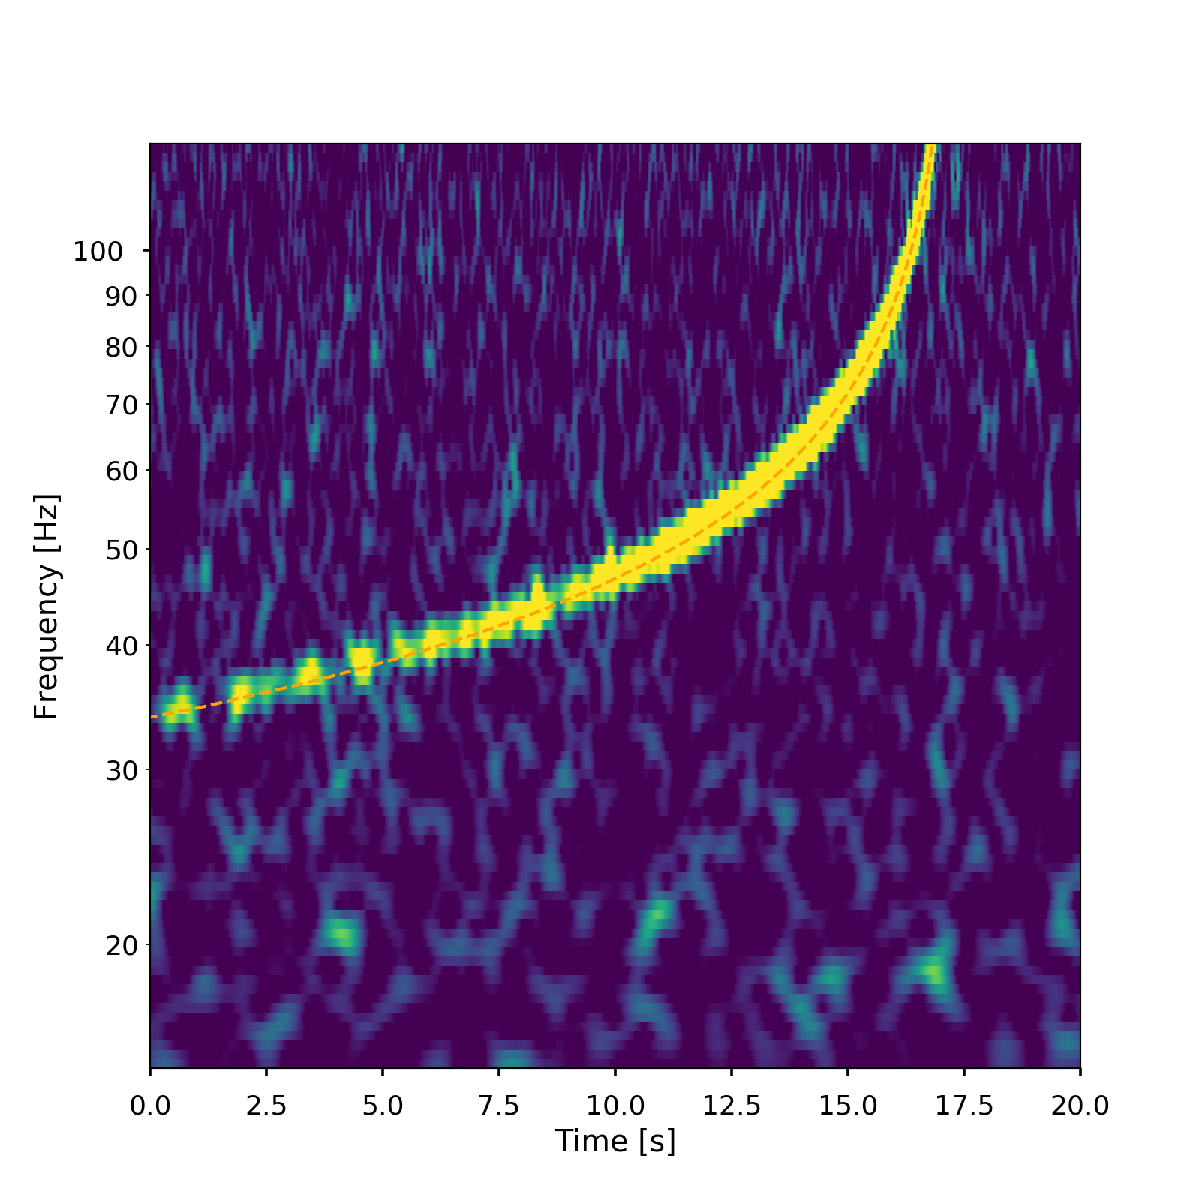
\includegraphics[width=0.49\linewidth]{Figures/Section3/3.8/L1_loud_Subtracted.pdf}
  \end{minipage}
    \caption{An injected binary neutron star compact binary coalescence \gw{} signal, with the \scl{} glitches identified by the ArchEnemy search pipeline overlayed in red (left). The same injected signal but with the \scl{} glitches removed from the data (right). It can be seen that power is removed from the signal track and also there is an amount of power added to the data above the track.}
    \label{fig:loud_inj}
\end{figure}

\section{\label{sec:results}Assessing sensitivity gain from removing \scl{} glitches}

We now assess whether removing our identified list of \scl{} glitches results in a sensitivity gain when searching for compact binary mergers. We do this by comparing the results from the offline PyCBC search on the original data, to the results of the same search but analysing data where the glitches have been removed.

\subsection{Comparing search results with and without glitch subtraction}

The PyCBC pipeline is able to assess significance of potential compact binary mergers in a given stretch of data, and does the same with a set of simulated signals. This significance is quoted in terms of a ``false-alarm rate'', which denotes how often we would expect to see a non-astrophysical event at least as significant as the coincident trigger being considered. In this work we assess sensitivity at a false-alarm threshold of 2 background events every year.

The data we have searched over contained no previously found \gw{} signals~\cite{gwtc3} and our search after subtracting \scl{} glitches identified no new \gw{} signals. While the search hasn't found any \gws{}, we can still measure the improvement in the sensitivity of the detectors by comparing the number of simulated signals identified with a false-alarm rate below 2 per year for each injection set (described in section~\ref{ssec:injsafety}) with and without removing glitches from the data. Table \ref{tab:found_injs} shows the number of injections found for all injection sets and both searches.
%
\begin{table}[tb]
\centering
\caption{\label{tab:found_injs}The number of injections found by each search with a false-alarm rate less than 2 per year alongside the number of newly-found and newly-missed injections, those found by the glitch-subtracted and not the original search and vice versa. We also show the sensitivity ratio of the glitch-subtracted search and original search for each injection set.} 
\footnotesize
\begin{tabular}{@{}cccccc}
\br
Injection & Original  & Glitch- & Sensitivity & Newly & Newly \\
Type & Search & Subtracted & ratio & Found & Missed \\
\mr
BBH           & 1215 & 1222 & 1.01 & 10 & 3\\
BNS           & 1315 & 1315 & 1.00 & 5 & 5 \\
NSBH          & 1260 & 1265 & 1.00 & 8 & 3 \\
\br
\end{tabular}

\end{table}

We compare the number of injections found by both searches but also look at the \gw{} injections found by the original search and missed by the glitch-subtracted search and vice versa, this information can be seen in table~\ref{tab:found_injs}. Considering signals found by the original search and missed by the glitch-subtracted search there are $3$ binary black hole injections with false-alarm rates in the original search ranging from $0.5 - 0.3$ per year, one of which had a glitch removed approximately $9$ seconds after the injection, there are $5$ newly-missed binary neutron star injections with false-alarm rates ranging from $0.5 - 0.056$ per year, two of the five binary neutron star injections had glitches removed within $60$ seconds of the injection, and there are $3$ newly-missed neutron star black hole injections with false-alarm rates ranging from $0.5 - 0.086$, one had glitches removed within $60$ seconds of the injection. The other newly-missed injections showed no \scl{} glitches within a $20$ second window for binary black hole injections and a $60$ second window for binary neutron star and neutron star black hole injections.

The glitch-subtracted search identifies $10$ additional binary black hole injections, the most significant of which have false-alarm rates of 1 per $190.50$, 1 per $7633.84$ and 1 per $8643.73$ years. We illustrate the last of these in figure~\ref{fig:ae_found} (top). $5$ extra binary neutron star injections were found, with false-alarm rates from $0.5 - 0.19$ per year and $8$ neutron star black hole injections were found, where the false-alarm rate of the most significant is 1 per $9961.55$ years. This injection can also be seen in figure~\ref{fig:ae_found} (bottom). We find $6$ of the $10$ binary black hole injections have \scl{} glitches within a $20$ second window of the injection, $3$ of $5$ binary neutron star injections have \scl{} glitches within a $60$ second window of the injection and, $6$ of the $8$ neutron star black hole injections have \scl{} glitches within a $60$ second window of the injection. We provide more details about the newly-found and newly-missed injections in~\ref{sec:apdx_injections_table}

\begin{figure}
  \centering
  \begin{minipage}[t]{1.0\linewidth}
    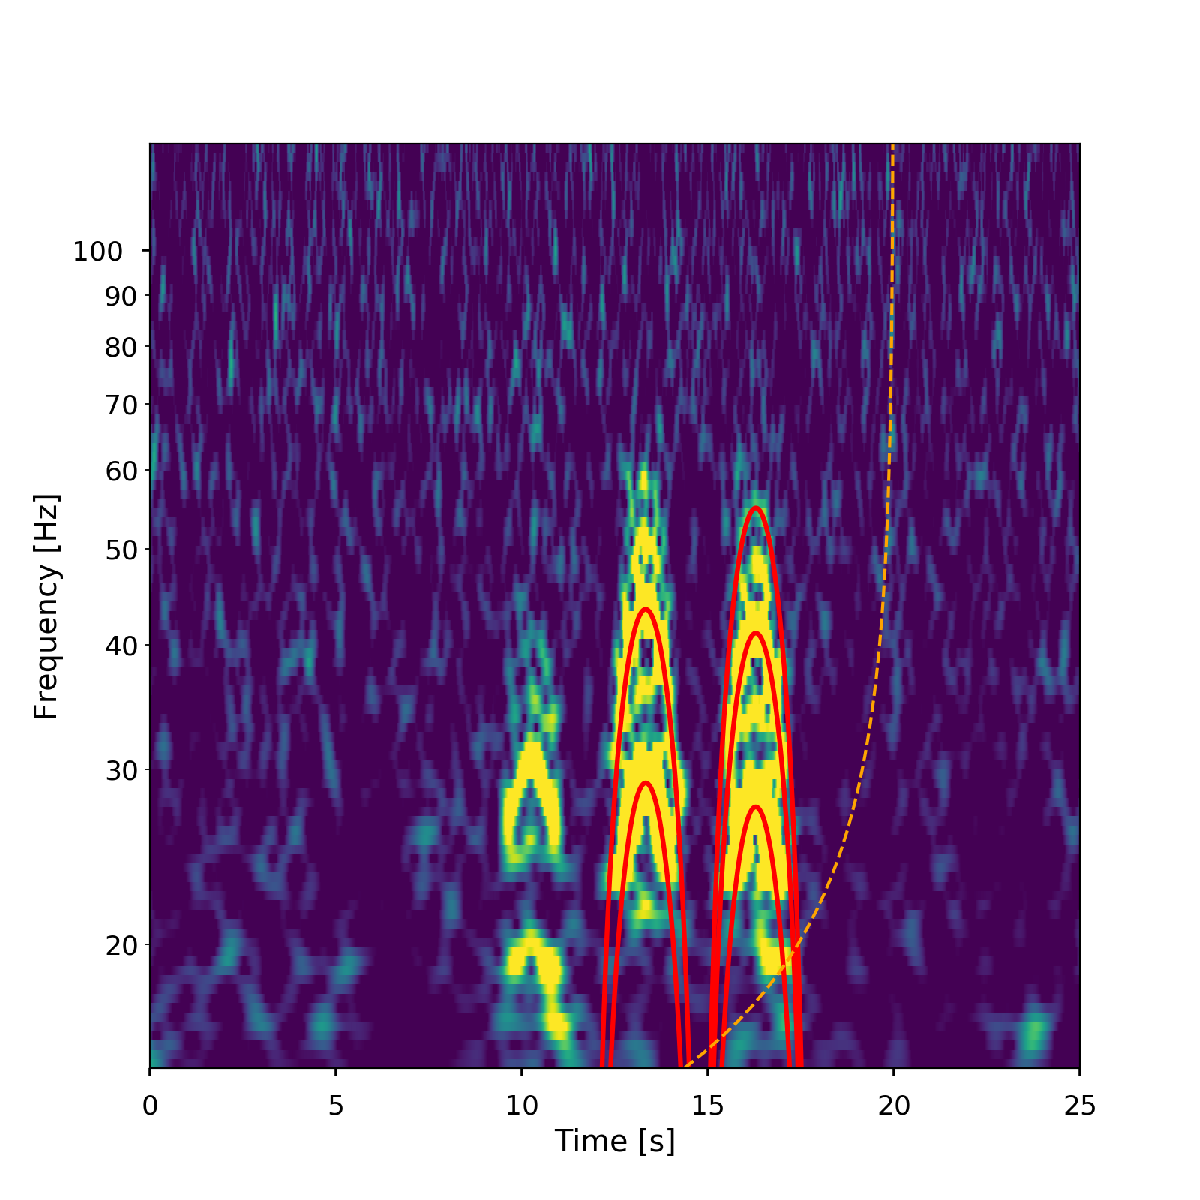
\includegraphics[width=0.49\linewidth]{Figures/Section4/4.1/ae_found_bbh/BBH_H1_loud_Original.pdf}
    \hspace{0.02\linewidth}
    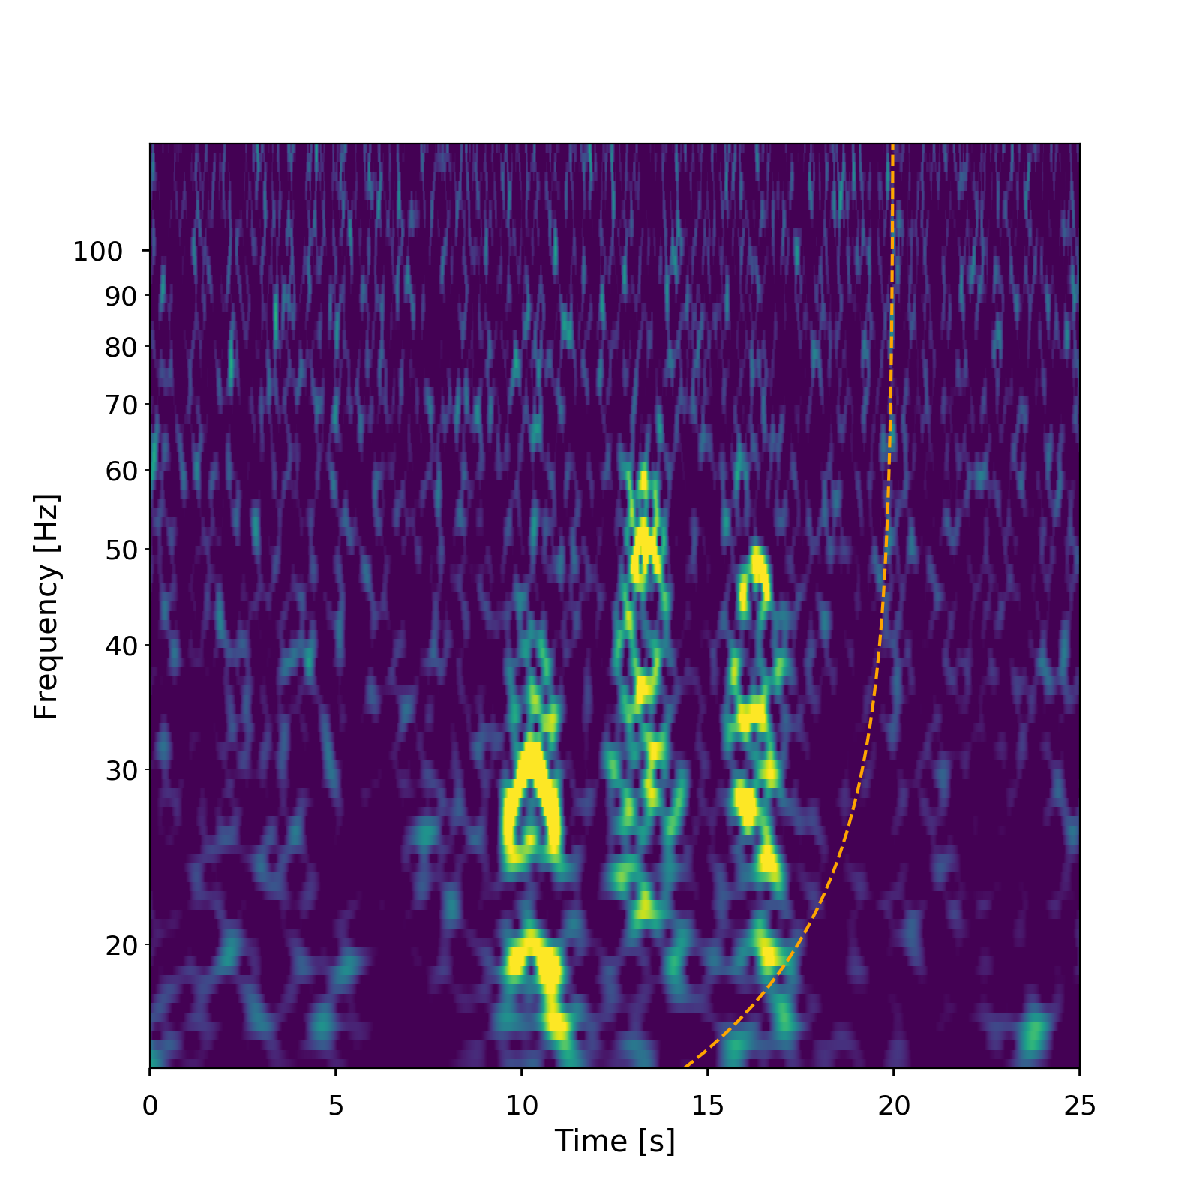
\includegraphics[width=0.49\linewidth]{Figures/Section4/4.1/ae_found_bbh/BBH_H1_loud_Subtracted.pdf}
  \end{minipage}
  \begin{minipage}[t]{1.0\linewidth}
    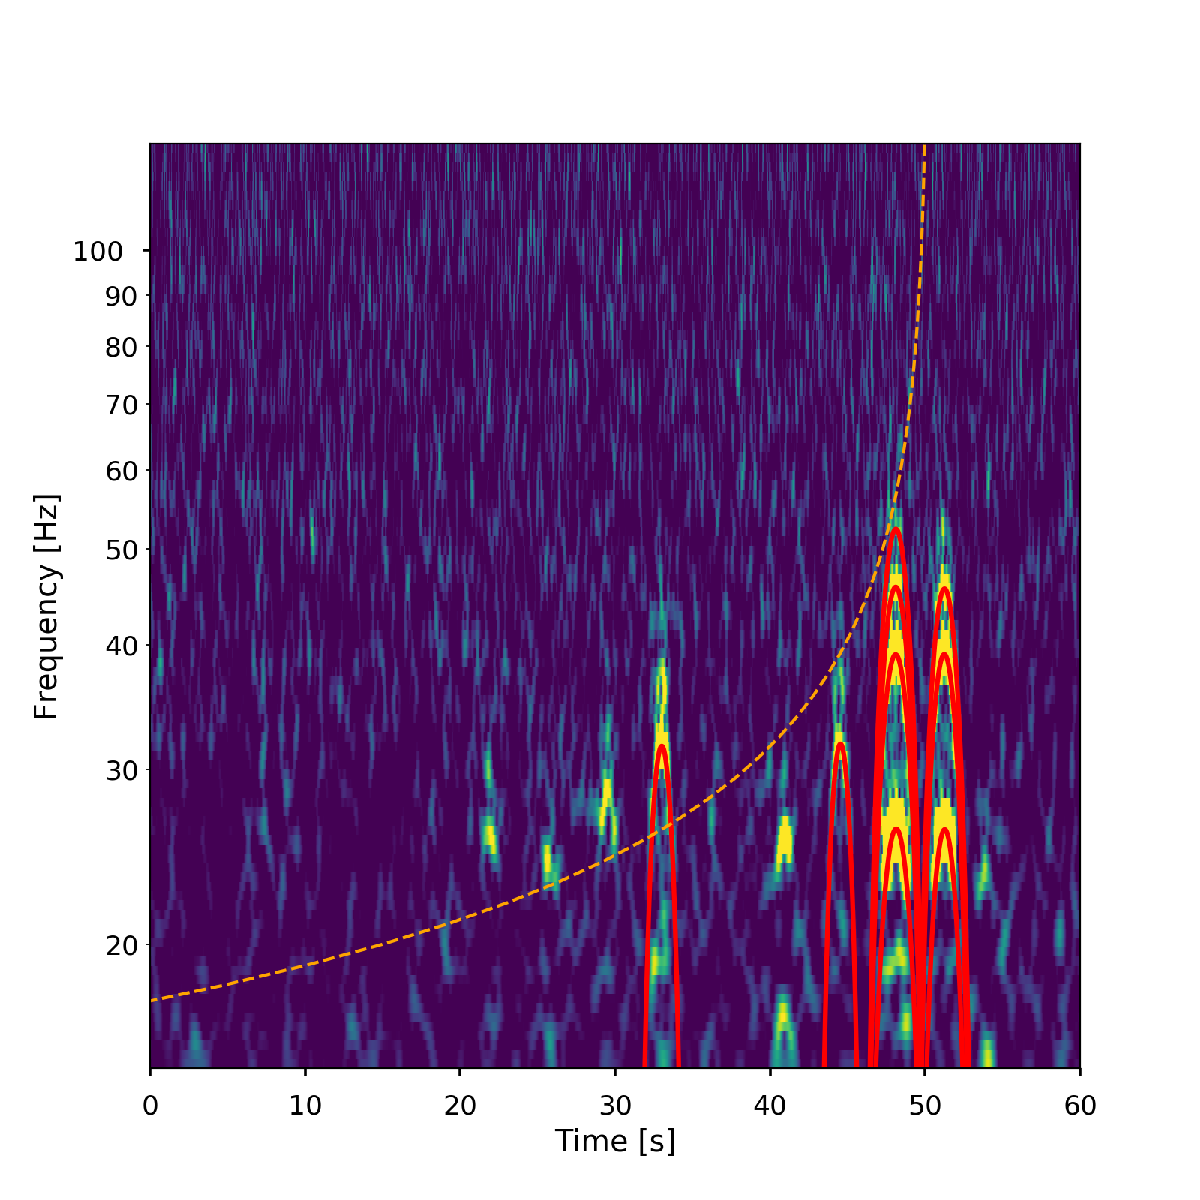
\includegraphics[width=0.49\linewidth]{Figures/Section4/4.1/ae_found_nsbh/NSBH_H1_loud_Original.pdf}
    \hspace{0.02\linewidth}
    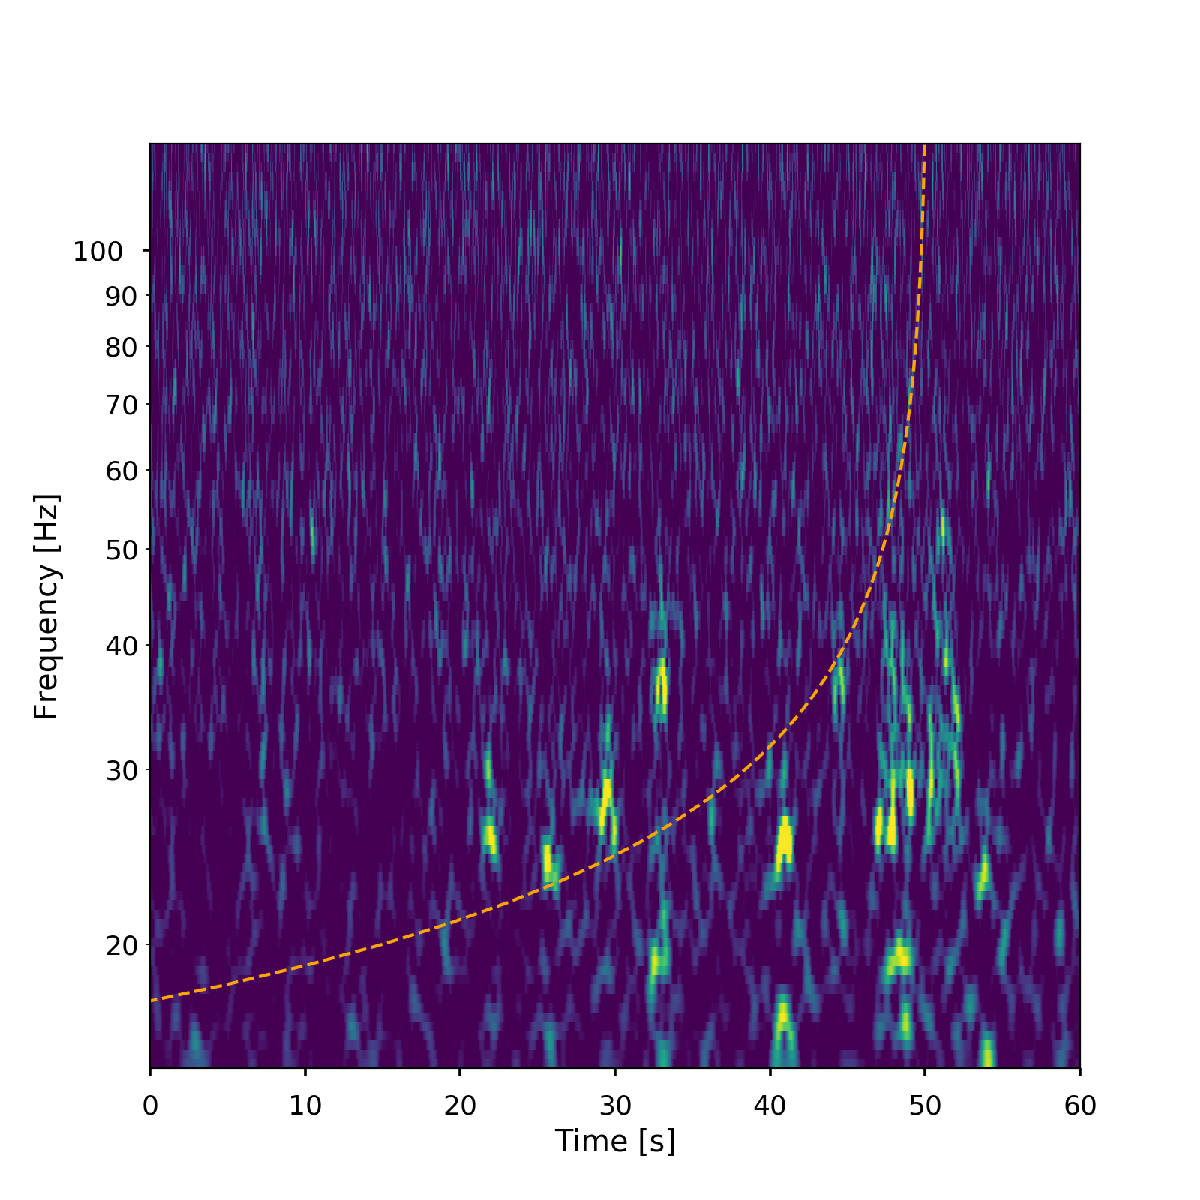
\includegraphics[width=0.49\linewidth]{Figures/Section4/4.1/ae_found_nsbh/NSBH_H1_loud_Subtracted.pdf}
  \end{minipage}
    \caption{Two examples of \gw{} injections found by the glitch-subtracted search for \gws{} which were not found by the original \gw{} search due to the presence of \scl{} glitches at the same time as the \gw{} inspiral. Top left: A binary black hole injection with a false-alarm rate of 1 per $8643.73$ years is shown alongside the \scl{} glitches found by the ArchEnemy search and subtracted from the data prior to performing the glitch-subtracted PyCBC search for \gws{} (top right). Bottom left: A neutron star black hole injection with a false-alarm rate of 1 per $9961.55$ years and the \scl{} glitches found by the ArchEnemy search and subtracted from the data prior to performing the glitch-subtracted PyCBC search for \gws{} (bottom right).}
    \label{fig:ae_found}
\end{figure}

To quantify the sensitivity of the search we calculate the sensitive volume in which we can observe \gw{} signals. To calculate the sensitive volume we measure the detection efficiency of different distance bins taken from the injection sets and then multiply the efficiencies by the volume enclosed by the distance bins, these volumes are then summed to find the total volume the search is sensitive to~\cite{rw_snr_eq}. We are then able to calculate the ratio in sensitivities between the glitch-subtracted \gw{} search and the original \gw{} search,  revealing the improvement that subtracting \scl{} glitches has made.

Figure~\ref{fig:allinj_vt_ratio} displays the ratio of the sensitive volume measured for the glitch-subtracted \gw{} search and the original PyCBC \gw{} search, across different false-alarm rate values, we quote our sensitivity ratios at a false-alarm rate value of 2 per year. The same set of injected signals was used for both \gw{} searches and therefore a direct comparison of search sensitivities can be made via this ratio. Disappointingly, the measured sensitivity improvement is small in the results we obtain. For the binary black hole injections we measure a sensitivity ratio at a 2 per year false-alarm rate of $1.01$, for binary neutron stars $1.00$ and neutron-star--black-holes $1.00$. 

The statistical significance of the sensitivity increase we report for the binary black hole injection set can be found by investigating the null hypothesis of seeing the same $1\%$ increase under the assumption that the subtraction of \scl{} glitches does not actually increase sensitivity. When performing this analysis we find that our result is not statistically significant at the 95\% confidence interval --i.e. there is a 5.24\% chance that we would measure such an increase in sensitivity at least as large as this under the null hypothesis-- (see~\ref{sec:apdx_stat_sig} for details). However, the marginal sensitivity increase would not justify repeating the \scl{} glitch search and glitch-subtracted \gw{} search on a larger injection set, instead more work is needed to better identify and remove \scl{} glitches while remaining safe in the presence of \gw{} signals.

\begin{figure}
     \centering
     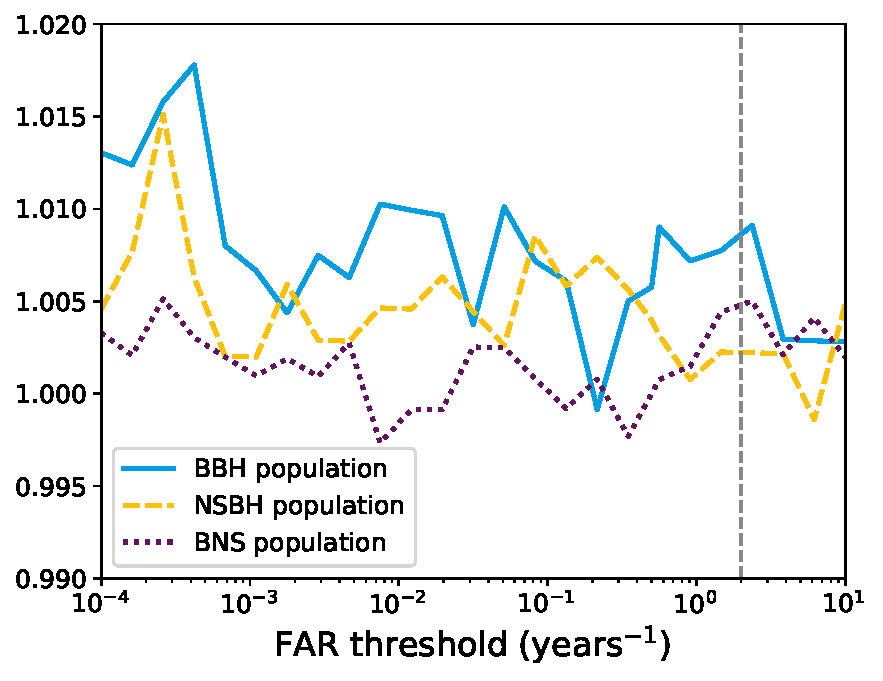
\includegraphics[width=0.7\textwidth]{Figures/Section4/4.1/allinj_vt_ratio_ArchEnemy_coinc.pdf}
     \caption{The ratio of the sensitive volume-time of the glitch-subtracted search and the original \gw{} search. The grey dashed line indicates a false-alarm rate of $2$ per year which is our threshold and the point at which we measure any sensitivity improvements of the glitch-subtracted search for each of the three \gw{} injection sets. }
     \label{fig:allinj_vt_ratio}
\end{figure}

\section{\label{sec:conclusion}Conclusion}

We have demonstrated a new method for modelling \scl{} glitches and identifying and characterizing these glitches in a period of \gw{} data. We have developed a \scl{} glitch specific $\chi^{2}$ test which can discriminate between \scl{} glitches, other types of glitches and \gw{} signals. We have searched through a representative stretch of \gw{} data known to contain \scl{} glitches, found thousands of these glitches and subtracted them from the \gw{} data prior to running a search for \gws{}. The results of this search include a small increase in the measured sensitivity of the \gw{} search for binary black hole \gw{} signals, and modest change to sensitivity for binary neutron star and neutron star black hole \gw{} signals.

We highlight that the task of accurately identifying and parameterizing \scl{} glitches in the data is not a trivial one, especially where there are repeated, and harmonic, glitches present in the data. We have developed a new $\chi^{2}$ test to reduce the number of false identifications of \scl{} glitches, but we do still see cases where we have misidentified other glitches, and even a small number of loud \gw{} signals, as caused by scattered light, and cases where we do not correctly identify, or parameterize, actual \scl{} glitches. Improving this identification process would be important in improving the efficacy of this process.

The possibility of using this model of \scl{} glitches as a bespoke application to \gw{} signals which are known to have coincident \scl{} glitches has been explored and implemented into Bilby~\cite{Bilby} to perform a parameter estimation of \scl{} glitches and removing these to produce glitch-free data~\cite{Udall2022}. The inclusion of the extra term from~\cite{MichalSub} within the model can help identify \scl{} glitches more accurately. Selectively subtracting glitches based on the presence of a \gw{} signal is possible by moving the glitch subtraction process inside of the \gw{} searches and including the results of other \gw{} discriminators~\cite{rw_snr_eq, McIsaac_2022} to determine the legitimacy of an ArchEnemy identified glitch.

The results of the application of the ArchEnemy search pipeline, the list of \scl{} glitches, can also be used in other applications. For example it could be used in the form of a veto~\cite{DetCharO2O3}, where we use knowledge of the presence of \scl{} glitches to down rank periods of time in \gw{} data. Additionally, we could use \scl{} glitches previously identified by tools such as Gravity Spy~\cite{GSpy2022} and target known \scl{} glitches with the ArchEnemy search pipeline.

As a final note, while we acknowledge that the sensitivity improvements that we have observed---$\sim 1\%$---are very modest, the concept of removing \scl{} glitches, or other identified glitch classes, from the data prior to matched filtering for compact binary mergers is one that we encourage others to explore further. An increase in the rate of events or the rate of \scl{} glitches in future observing runs will mean an increase in the number of affected events, such techniques offer a method for mitigating the effect that these glitches will have on the search, maximizing the number of observations that can be made.
%
%%%%%%%%%%%%%%%%%%%%%%%%%%%%%%%%%%%%%%%%%%%%%%%%%%%%%%%%%%%%%%%%%%%%%%%%%%%%%%%%%%%%%%%%%%%%%%%%%%%
\section{\label{sec:apdx_stat_sig}Statistical Significance}

We report a $1\%$ increase in the sensitivity for the binary black hole injection set in the glitch-subtracted \gw{} search (see section~\ref{sec:results}). We wish to determine the statistical significance of this result under the null hypothesis that subtracting \scl{} glitches prior to searching for \gws{} does not increase the sensitivity of the \gw{} search. The binary black hole injection set contains $6200$ injected signals, $10$ additional injections were found in the glitch-subtracted \gw{} search, $3$ additional injections were missed in our search, this gives us $13$ injections which have changed state.

First, we calculate the probability that an injection has been affected by the glitch removal, 
%
\begin{equation}
    p = \frac{13}{6200} = 0.21\% ,
\end{equation}
%
then we calculate the standard deviation, 
%
\begin{equation}
    \textrm{std} = \sqrt{n * p * (1 - p)} = 3.60 .
\end{equation}
%
Using the standard deviation we calculate the number of standard deviations our result deviates from the mean. We divide the number of positively changed (newly-found) injections by the standard deviation, 
%
\begin{equation}
    \textrm{standard deviations} = \frac{(10 - 3)}{3.60} = 1.94 .
\end{equation}
%
Under the assumption of no sensitivity increase caused by the subtraction of glitches, we measure our result of +7 newly-found \gw{} injections to lie $1.94$ standard deviations from an expected value of $0$ newly-found injections. The critical value of a 95\% confidence interval, that is to say there is a 1 in 20 chance of our null hypothesis being true, is $1.96$ meaning our result is within the 95\% confidence interval. We can describe this as there being a 5.24\% chance that our result is not caused by the subtraction of glitches but is instead caused by random chance. To reduce the error in the computed sensitivity ratio a larger injection set test would be required, this would need a large time and computational power investment which we do not believe is justified in the case of such a minor increase in the sensitivity.

\section{\label{sec:apdx_injections_table}}

Here we have three tables which contain data on the newly-found and newly-missed injections for each injection set. The tables are separated into the values for the inverse false-alarm rate and ranking statistic found for each injection in both searches then the signal-to-noise ratio, $\chi^{2}$ and PSD variation values for each detector in both searches. The first table is the results of the binary black hole injection set, the second table is the binary neutron star injection set and the third is the neutron star black hole injection set. A horizontal dashed line separates newly-found and newly-missed injections, using a false-alarm rate threshold of 2 per year. There were 2 newly-found binary black hole injections which were not found at all by the original search and therefore they do not appear in the first table.

There have been 34 newly-found or newly-missed \gw{} injections when subtracting \scl{} glitches, it is informative to understand how the \gw{} search is influenced by the glitch subtraction to cause this outcome. The ranking statistic~\cite{Davies:2020tsx} represents the legitimacy of a signal being astrophysical in origin and is partially computed using the re-weighted signal-to-noise ratio, which is itself computed using the initial signal-to-noise ratio alongside the various \gw{} discriminators and the PSD variation measurement~\cite{Mozzon_2020}. We use the trigger information saved by the \gw{} search to identify why injections that weren't found previously have been found post-glitch subtraction, and vice versa. 

As an example, we take the smallest false-alarm rate (1 per $8643.73$ years), newly-found, binary black hole injection, and look at the ranking statistic, signal-to-noise ratio, $\chi^{2}$ and, PSD variation measurements in both detectors and both searches -- these values can be found in table~\ref{tab:apdx_changed_snr_bbh}. This injection was originally seen with a false-alarm rate of 100 per year, far above our threshold, a very large increase in the ranking statistic from 13.29 to 27.01 is certainly responsible for the decreased false-alarm rate. There were no changes in the values measured by the LIGO-Livingston detector between searches which is expected as no \scl{} glitches were found within $512$ seconds of the injection. The LIGO-Hanford detector sees a small increase in the signal-to-noise ratio measured, from 7.98 to 8.22, a small increase in the $\chi^{2}$ value, from 2.32 to 2.48, and a very significant decrease in the PSD variation measurement, from 3.47 to 1.50. Using equation 18 of~\cite{Mozzon_2020}, we can calculate a re-weighted signal-to-noise ratio of $4.60$ for the original search and $5.67$ for the glitch-subtracted search, a significant increase in the signal-to-noise ratio. Similar analyses for all the newly-found and newly-missed injections can be made using information found in tables~\ref{tab:apdx_changed_snr_bns} and~\ref{tab:apdx_changed_snr_nsbh}.

The decrease in the PSD variation is true for the three newly-found very low false-alarm rate injections, accompanied by the small changes in signal-to-noise ratio and increase in the $\chi^{2}$ measurement. For newly-found and newly-missed injections which lie close to the 2 per year false-alarm rate threshold there is no definitive reason as to why these injections changed state.

\newpage
\newgeometry{left=2cm,right=2cm,top=2cm,bottom=2cm} % set new margins for one page
\begin{landscape}
\begin{table}[tb]
\centering
\caption{\label{tab:apdx_changed_snr_bbh}This table contains the trigger information for the newly-found and newly-missed \textbf{binary black hole injections} recorded by the original search~\cite{gwtc3} and the glitch-subtracted search.} 
\begin{tabular}{|c|c|c|c|c|c|c|c||c|c|c|c|c|c|c|c|}
\hline
\multicolumn{8}{|c||}{Glitch-Subtracted} & \multicolumn{8}{c|}{Original Search} \\
\hline
\multicolumn{2}{|c|}{} & \multicolumn{3}{c|}{H1} & \multicolumn{3}{c||}{L1} & \multicolumn{2}{c|}{} & \multicolumn{3}{c|}{H1} & \multicolumn{3}{c|}{L1}\\
\hline
IFAR & Ranking & SNR & $\chi^{2}$ & PSD & SNR & $\chi^{2}$ & PSD & IFAR & Ranking & SNR & $\chi^{2}$ & PSD & SNR & $\chi^{2}$ & PSD \\ &

Stat. & & & Var. & & & Var. & & Stat. & & & Var. & & & Var.\\
\hline
8643.73 & 27.01 & 8.22 & 2.48 & 1.50 & 8.05 & 2.07 & 1.00 & 0.01 & 13.29 & 7.98 & 2.32 & 3.47 & 8.05 & 2.07 & 1.00 \\
7633.84 & 26.13 & 8.18 & 2.25 & 1.22 & 7.58 & 1.46 & 1.03 & 0.37 & 16.63 & 8.19 & 1.87 & 2.17 & 7.59 & 1.45 & 1.02 \\
4.89 & 19.06 & 7.23 & 1.88 & 0.97 & 10.34 & 3.15 & 1.05 & 1.56 & 18.01 & 7.24 & 2.11 & 0.97 & 10.34 & 3.42 & 1.04 \\
3.14 & 18.65 & 5.89 & 1.54 & 1.01 & 8.86 & 2.40 & 1.09 & 1.52 & 17.99 & 5.89 & 1.54 & 1.01 & 8.86 & 2.40 & 1.09 \\
2.75 & 18.53 & 8.50 & 1.63 & 0.99 & 6.80 & 1.37 & 1.05 & 1.51 & 17.98 & 8.51 & 1.56 & 0.98 & 6.80 & 1.37 & 1.05 \\
2.39 & 18.41 & 7.83 & 2.00 & 1.01 & 8.41 & 3.41 & 1.02 & 1.06 & 17.65 & 7.81 & 2.14 & 1.01 & 8.41 & 3.41 & 1.02 \\
2.18 & 18.32 & 7.02 & 1.90 & 1.02 & 6.35 & 2.15 & 1.01 & 1.79 & 18.14 & 7.05 & 1.92 & 1.02 & 6.35 & 2.16 & 1.01 \\
2.01 & 14.11 & 7.94 & 1.89 & 1.01 & 5.67 & 1.95 & 1.16 & 1.90 & 14.14 & 7.94 & 1.90 & 1.01 & 5.07 & 0.00 & 1.02 \\
\hdashline
1.76 & 18.12 & 6.89 & 1.43 & 1.02 & 6.76 & 2.59 & 0.97 & 3.33 & 18.71 & 6.86 & 1.82 & 1.02 & 6.68 & 2.53 & 0.97 \\
1.79 & 18.14 & 6.40 & 1.69 & 1.02 & 7.56 & 2.01 & 1.01 & 2.05 & 18.27 & 6.40 & 1.69 & 1.02 & 7.56 & 2.00 & 1.01 \\
1.65 & 18.06 & 5.14 & 0.00 & 0.91 & 7.57 & 1.57 & 1.02 & 2.05 & 18.27 & 5.14 & 0.00 & 0.91 & 7.57 & 1.57 & 1.02 \\
\hline
\end{tabular}
\end{table}
\end{landscape}
\restoregeometry % restore the default margins for subsequent pages

\newpage

\newgeometry{left=1cm,right=1cm,top=2cm,bottom=2cm} % set new margins for one page
\begin{landscape}
\begin{table}[tb]
\centering
\caption{\label{tab:apdx_changed_snr_bns}This table contains the trigger information for the newly-found and newly-missed \textbf{binary neutron star injections} recorded by the original search~\cite{gwtc3} and the glitch-subtracted search.} 
\begin{tabular}{|c|c|c|c|c|c|c|c||c|c|c|c|c|c|c|c|}
\hline
\multicolumn{8}{|c||}{Glitch-Subtracted} & \multicolumn{8}{c|}{Original Search} \\
\hline
\multicolumn{2}{|c|}{} & \multicolumn{3}{c|}{H1} & \multicolumn{3}{c||}{L1} & \multicolumn{2}{c|}{} & \multicolumn{3}{c|}{H1} & \multicolumn{3}{c|}{L1}\\
\hline
IFAR & Ranking & SNR & $\chi^{2}$ & PSD & SNR & $\chi^{2}$ & PSD & IFAR & Ranking & SNR & $\chi^{2}$ & PSD & SNR & $\chi^{2}$ & PSD \\ &
Stat. & & & Var. & & & Var. & & Stat. & & & Var. & & & Var.\\
\hline
5.12 & 19.12 & 5.86 & 1.99 & 1.01 & 7.15 & 1.94 & 1.02 & 1.49 & 17.96 & 5.74 & 2.14 & 1.01 & 7.15 & 1.94 & 1.02 \\
4.91 & 19.07 & 5.48 & 2.29 & 1.01 & 7.92 & 2.16 & 1.01 & 1.37 & 17.89 & 5.78 & 2.25 & 1.01 & 7.23 & 2.13 & 1.01 \\
4.54 & 18.99 & 4.82 & 0.00 & 1.07 & 8.68 & 2.05 & 1.06 & 1.66 & 18.07 & 4.82 & 0.00 & 1.14 & 8.68 & 2.05 & 1.06 \\
2.46 & 18.43 & 5.48 & 1.95 & 1.05 & 7.61 & 2.03 & 0.99 & 1.78 & 18.13 & 5.48 & 1.94 & 1.05 & 7.62 & 2.08 & 0.99 \\
2.34 & 18.39 & 6.25 & 2.18 & 1.01 & 6.82 & 1.96 & 1.00 & 1.45 & 17.94 & 6.09 & 2.05 & 1.01 & 6.83 & 2.01 & 1.00 \\
\hdashline
1.24 & 17.71 & 6.58 & 2.14 & 1.01 & 6.89 & 2.48 & 1.01 & 17.81 & 20.19 & 6.58 & 2.15 & 1.01 & 7.16 & 2.26 & 1.01 \\
1.14 & 17.72 & 6.00 & 2.67 & 0.98 & 8.07 & 2.66 & 1.22 & 7.14 & 19.44 & 6.17 & 2.45 & 0.97 & 8.26 & 2.80 & 1.22 \\
1.89 & 18.19 & 6.32 & 2.19 & 1.00 & 6.79 & 1.83 & 0.99 & 3.57 & 18.78 & 6.37 & 2.12 & 0.99 & 6.79 & 1.75 & 0.99 \\
0.88 & 17.46 & 6.88 & 2.14 & 0.99 & 6.19 & 2.12 & 0.99 & 2.33 & 18.39 & 6.87 & 2.07 & 0.99 & 6.19 & 1.99 & 0.99 \\
1.36 & 17.80 & 6.20 & 2.02 & 1.00 & 6.83 & 2.35 & 1.00 & 2.07 & 18.18 & 6.20 & 2.02 & 1.00 & 6.83 & 2.28 & 1.00 \\
\hline
\end{tabular}
\end{table}
\end{landscape}
\restoregeometry % restore the default margins for subsequent pages

\newpage

\newgeometry{left=1cm,right=1cm,top=2cm,bottom=2cm} % set new margins for one page
\begin{landscape}
\begin{table}[tb]
\centering
\caption{\label{tab:apdx_changed_snr_nsbh}This table contains the trigger information for the newly-found and newly-missed \textbf{neutron star black hole injections} recorded by the original search~\cite{gwtc3} and the glitch-subtracted search.} 
\begin{tabular}{|c|c|c|c|c|c|c|c||c|c|c|c|c|c|c|c|}
\hline
\multicolumn{8}{|c||}{Glitch-Subtracted} & \multicolumn{8}{c|}{Original Search} \\
\hline
\multicolumn{2}{|c|}{} & \multicolumn{3}{c|}{H1} & \multicolumn{3}{c||}{L1} & \multicolumn{2}{c|}{} & \multicolumn{3}{c|}{H1} & \multicolumn{3}{c|}{L1}\\
\hline
IFAR & Ranking & SNR & $\chi^{2}$ & PSD & SNR & $\chi^{2}$ & PSD & IFAR & Ranking & SNR & $\chi^{2}$ & PSD & SNR & $\chi^{2}$ & PSD \\ &
Stat. & & & Var. & & & Var. & & Stat. & & & Var. & & & Var.\\
\hline
9961.55 & 27.41 & 5.55 & 2.08 & 1.23 & 10.26 & 2.27 & 1.12 & 0.01 & 12.83 & 6.01 & 2.39 & 2.25 & 8.54 & 2.37 & 1.12 \\
141.35 & 22.28 & 7.76 & 2.20 & 1.02 & 6.54 & 2.35 & 1.01 & 1.21 & 17.77 & 7.83 & 1.94 & 1.02 & 7.29 & 2.50 & 1.00 \\
18.26 & 20.36 & 5.94 & 2.20 & 1.09 & 6.02 & 1.99 & 1.10 & 1.29 & 17.82 & 5.74 & 2.05 & 1.09 & 6.27 & 2.10 & 1.18 \\
17.12 & 20.29 & 7.64 & 2.00 & 1.11 & 6.66 & 2.15 & 1.05 & 1.37 & 17.89 & 7.36 & 2.35 & 1.11 & 6.66 & 2.15 & 1.05 \\
12.94 & 20.03 & 6.52 & 1.79 & 1.07 & 7.31 & 2.32 & 1.13 & 1.96 & 18.23 & 6.57 & 1.85 & 1.20 & 7.31 & 2.32 & 1.13 \\
7.12 & 19.42 & 5.13 & 0.00 & 1.05 & 8.33 & 2.08 & 1.04 & 0.03 & 14.23 & 5.30 & 2.16 & 1.05 & 7.44 & 2.43 & 1.04 \\
3.61 & 18.77 & 5.80 & 2.01 & 1.02 & 7.43 & 1.88 & 0.93 & 1.81 & 18.15 & 5.80 & 2.01 & 1.02 & 7.43 & 1.97 & 0.93 \\
2.15 & 18.22 & 7.41 & 2.04 & 1.02 & 5.57 & 2.03 & 1.03 & 0.00 & 4.34 & 5.64 & 2.18 & 0.98 & 5.04 & -0.00 & 1.01 \\
\hdashline
0.23 & 16.16 & 5.79 & 1.81 & 0.96 & 8.78 & 3.93 & 1.03 & 11.69 & 19.93 & 5.78 & 1.89 & 0.96 & 8.79 & 3.17 & 1.03 \\
1.56 & 17.92 & 6.71 & 1.91 & 0.99 & 6.73 & 2.50 & 1.05 & 2.68 & 18.41 & 6.71 & 1.90 & 0.99 & 6.72 & 2.39 & 1.05 \\
1.72 & 18.10 & 5.77 & 1.90 & 0.99 & 6.77 & 1.74 & 1.00 & 2.08 & 18.28 & 5.77 & 1.90 & 0.99 & 6.80 & 1.69 & 1.00 \\
\hline
\end{tabular}
\end{table}
\end{landscape}
\restoregeometry % restore the default margins for subsequent pages

%%begin novalidate


%---% PyCBC Live Ranking Statistic %---%
\chapter{Improving the PyCBC Live Ranking Statistic}
% Introduce the chapters contents
%   Previous PyCBC Live Ranking Statistic
%   New Additions
%   PSD Var
%   Template Fits
%   Testing - Injection Tests
%   Sensitivity Increase


In this chapter we discuss the improvements made to the PyCBC Live search's ranking statistic which has enabled an increase in the sensitivity of the live search of over 30\%. We will discuss the new additions to the ranking statistic and how these have been adapted for the live search.

\section{\label{live-previous-stat}Previous Ranking Statistic}

As mentioned in~\ref{sec:live-ranking-statistic} PyCBC Live used the same ranking statistic during both the third observing run and the first half of the fourth observing run.

The ranking statistic can be split into two components: a single trigger ranking statistic and a coincident trigger ranking statistic. The single trigger ranking statistic used in PyCBC Live was \verb|newsnr_sgveto|, where \verb|newsnr| refers to the calculation of a new SNR value that has been weighted by the chisq value calculated using the Allen chisq and, \verb|sgveto| is the same re-weighting but for another chisq called the sine-gaussian chisq.

The coincident ranking statistic used was \verb|phasetd| which is the simplest coincident ranking statistic, checking only phase and time consistency of the triggers in separate detectors to ensure they arrived within the physical light travel time and with the same phase state.

\section{\label{live-new-additions}New Additions}

To improve the ranking statistic we have included two new components which are currently used in the PyCBC offline ranking statistic: PSD variation and template fits. These two components have been previously described in sections~\ref{sec:psd-variation}~\&~\ref{sec:template-fitting}.

\subsection{\label{live-psd-var}PSD Variation in Live}

% Section introduction
We have described the theory of PSD variation in section~\ref{sec:psd-variation} and in this section we will describe the implementation of PSD variation in the live search and how this differs from that of the offline search.

% Brief explanation of PSD variation
The PSD measures the power distribution of the data in the frequency domain, when this PSD is inaccurate it can cause inaccurately measured SNR values for a trigger. PSD variation is a measure of the difference between the true PSD of the data and the estimated PSD being used by the search.

% PSD variation in offline
The PyCBC offline search for gravitational waves searches through 512 seconds of data in each chunk. The PSD for this chunk is measured once and used for the whole stretch of time, this can be inaccurate for different points of time in the whole chunk. The offline search therefore measures the PSD variation at each second and when a trigger is found the variation value is found by interpolating between the two nearest seconds.

% Difference between offline and live
The PyCBC live search in contrast maintains a buffer of 256 seconds of data, rolling the newest eight seconds on as the oldest eight second are rolled off. The PSD of this data is measured and the neutron star binary distance is calculated, the PSD is then re-estimated regularly and if the neutron star binary distance of a newly estimated PSD is greater than a 1\% difference to the current PSD then the current PSD is updated to this new PSD. This reduces the effect of a poorly estimated PSD but there is still some potential for non-stationary data to effect the search. 

% How we calculate the PSD var in live?
The offline search computes the PSD variation values for the whole chunk in one go. If the live search were to do the same it would have to compute the PSD variation values every eight seconds for the whole 256 second chunk of data. This would mean that each second would be calculated 32 times as it makes its way through the buffer, wasted computing resources and introducing lag to the search. Instead, the live search only calculates the PSD variation for the latest eight seconds of data, as this is the same time when there will any new triggers for the PSD variation to get assigned to. These PSD variation values are then saved with the triggers and the memory is re-allocated for the next set epoch of the search.

\subsection{\label{live-template-fits}Template Fits}

The offline search takes the previous week (CHECK) of triggers and create the statistic files required for the template fits. This process is identical in the live search's implementation of the template fits except for the triggers need to be collated from the individual trigger files produced every eight seconds and then they need to be converted to the format required to produce the template fits files.
%
\begin{figure}
  \centering
  \begin{minipage}[t]{1.0\linewidth}
  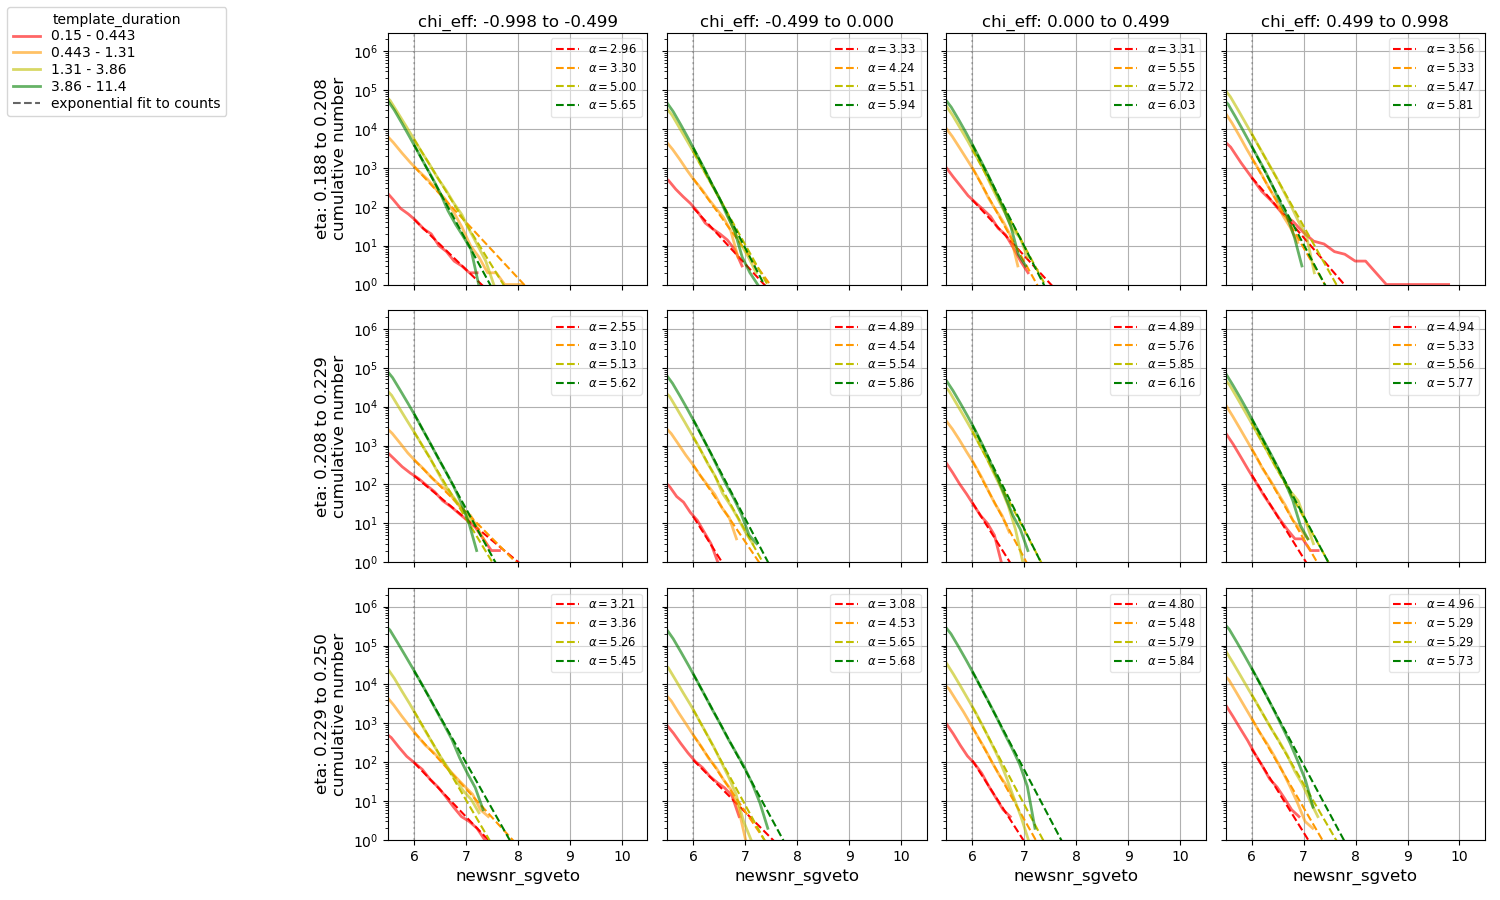
\includegraphics[width=0.49\textwidth]{images/pycbclive/H1-template_fits.png}
  \hspace{0.01\linewidth}
  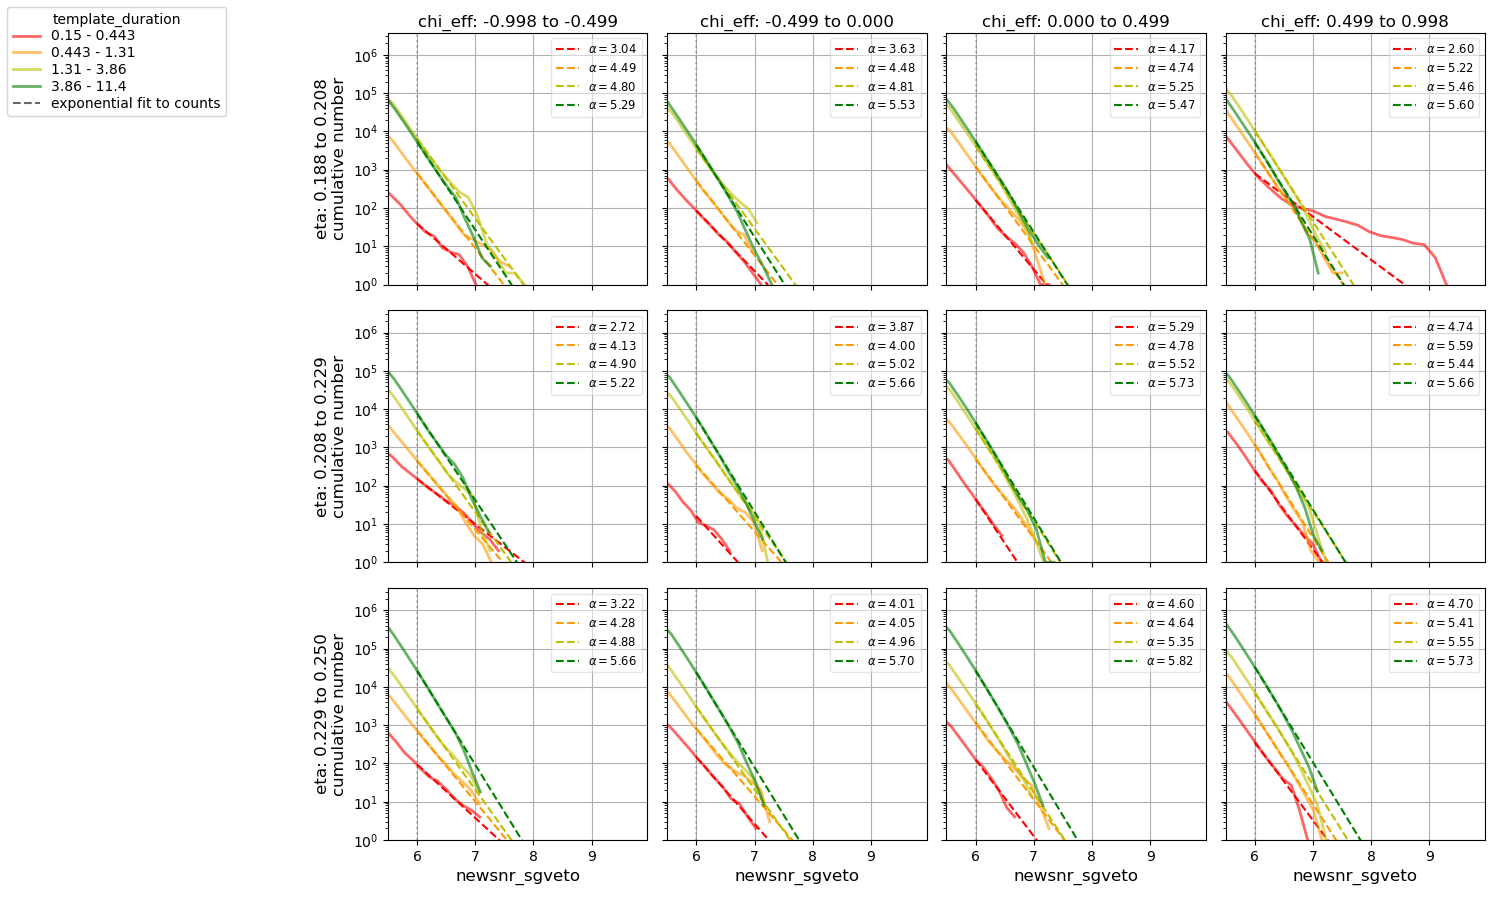
\includegraphics[width=0.49\linewidth]{images/pycbclive/L1-template_fits.png}
  \end{minipage}
  \caption{}
  \label{fig:pycbclive-fits}
\end{figure}
%
Figure~\ref{fig:pycbclive-fits} shows the associated fits made by the injection testing we did to measure the increase in sensitivity. These fits show good agreement to the exponential in the majority of the template bins except for the top-right for both H1 and L1 where there is an excess of high SNR triggers for these high-chieff, low eta and very short duration BBH templates.

\section{\label{sec:pcycblive-sensitivity-improvements}Sensitivity Improvements}

We measure improvement to the live search by performing injection set tests. The injection sets are made up of thousands of gravitational wave signals that are injected at a rate of approximately one every 100 seconds. We run two 'live' searches for gravitational waves, one with the old ranking statistic and one with the new ranking statistic which includes the additions of both PSD variation and template fitting.

The injection set used for this test is made up entirely of BBH signals to reduce the size of the template bank required~(CITE R\&P PAPER FOR O3), there is a limit to the amount of memory a user can request for this pseudo-live search and therefore we couldn't initially test these changes on the full pycbc live template bank. The template bank of 15436 templates covers the BBH signal parameter space and is described in this paper~(CITE O3 BBH PAPER?). 

The gravitational wave data used was a two week period of O3b where the first week was used to generate the template fits and the second week was used to test the fits. The injected gravitational wave data was created before the live searches were run and both searches were run on exactly the same data. While this search is emulating the live search it will very simply wait for new data before it moves forwards by eight seconds, if this data already exists (in the form of pregenerated data) then it will perform the processing as fast as it can. Therefore, a running the live search over a week of data does not take a whole week but it can take as little as 24 hours.

Once both searches have completed we can count the number of injections found by both searches. Theoretically the searches should both observe the exact same number of injections with almost identical triggers due to their nature but, computing isn't always perfect and therefore the searches observed slightly different amounts of time during the second week. This means that a simple count of injections found cannot be done, we need to isolate the injections seen in jointly observed time between the two searches.

This produced a list of injections seen by both searches in which we can directly compare the false alarm rate (or inverse false alarm rate, IFAR) of each injection to see if there has been an improvement. Each of these events is a real gravitational wave signal so we hope to see every single injection with a large IFAR value to indicate that the changes to the ranking statistic has improved the sensitivity of the search. Figure~\ref{fig:pycbclive-ifar-vs-ifar} displays the change in IFAR for each injection with the new statistic (colloquially referred to as 'fits') on the y-axis and the x-axis the old statistic IFAR values.
%
\begin{figure}
       \centering
    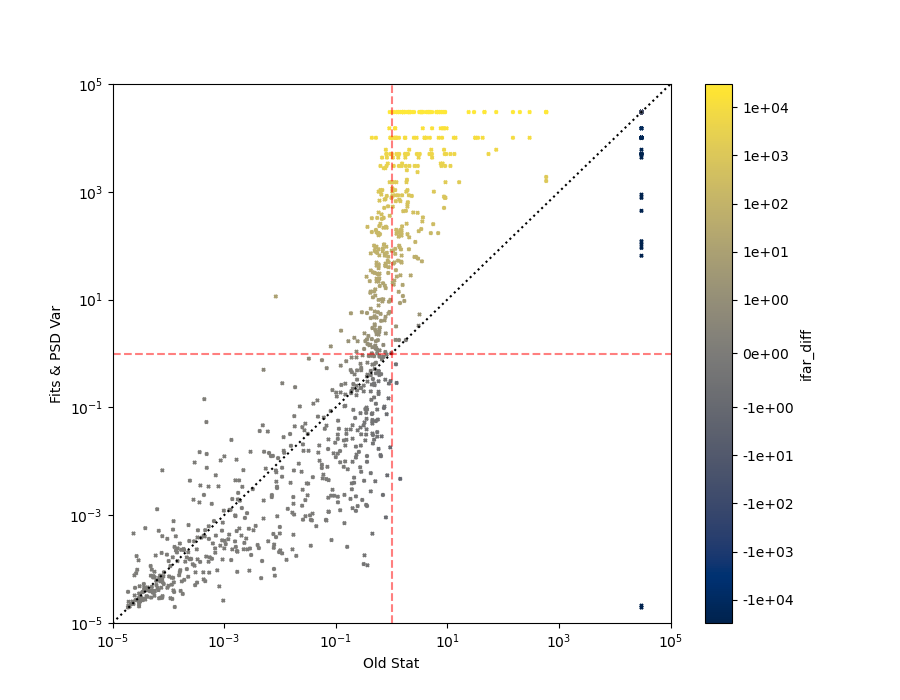
\includegraphics[width=1.2\textwidth]{images/pycbclive/fits_vs_old_colour.png}
    \caption{}
    \label{fig:pycbclive-ifar-vs-ifar}
\end{figure}
%
Within figure~\ref{fig:pycbclive-ifar-vs-ifar} we have plotted a vertical and horizontal dotted line at an IFAR of 1 year to indicate a commonly chosen IFAR limit of where an event would be considered 'real'. Therefore this figure can be split into four quadrants: top-left, injections originally missed below the IFAR threshold and now found above it; top-right, injections found in both searches; bottom-left, injections below the threshold by both searches; bottom-right, injections originally found above the IFAR threshold but missed with the new statistic. Another line has been plotted at y=x, injections above this line (in the top-left) have been found with a larger IFAR with the new statistics and injections below (in the bottom-right) have been found with a lower IFAR with the new statistic.

We have investigated all injections in the bottom-right quadrant and have found discrepancies in why these have been down-ranked which needs further investigation.

To measure the sensitivity improvements of the new statistic we count the number of injections found with IFAR over a certain number for both searches. If we do this for a range of IFAR values then we can build up an image of the sensitivity increase when using the new statistic. Figure~\ref{fig:pycbclive-sensitivity} shows this ratio of new statistic over old statistic.
%
\begin{figure}
       \centering
    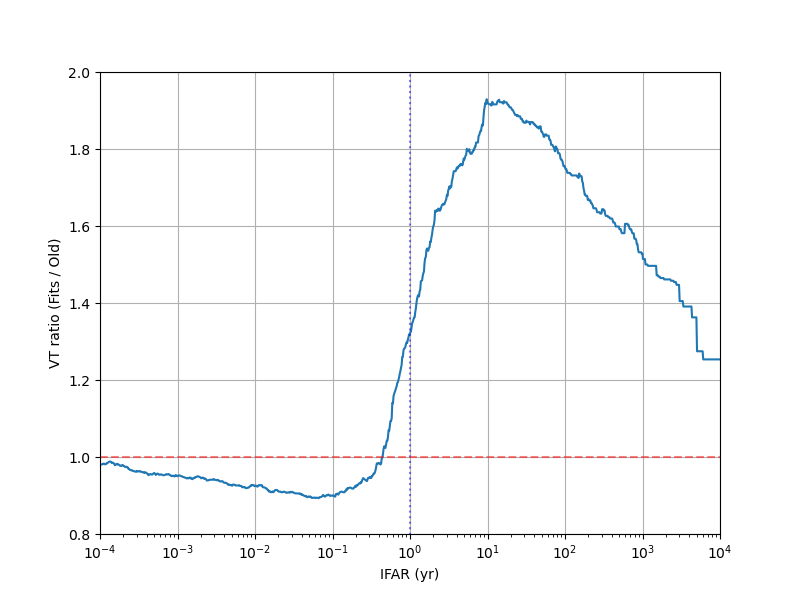
\includegraphics[width=1.0\textwidth]{images/pycbclive/ratio.png}
    \caption{}
    \label{fig:pycbclive-sensitivity}
\end{figure}
%
The new statistic at an IFAR of 1 year can be seen to have found approximately 35\% more gravitational wave signals with an IFAR greater than 1 year. This is a large increase and demonstrates the benefit of adding the PSD variation and templates fits to the live search.




%---% Early Warning Ranking Statistic %---%
\chapter{Early Warning Ranking Statistic}
\section{The Motivation of Multi-Messenger Astronomy}

The previous five chapters of this thesis have demonstrated the capabilities of the gravitational wave detectors and searches and how the field of gravitational wave astronomy has observed events which had previously never been seen. This chapter will cover how gravitational wave astronomy can be paired with traditional electromagnetic astronomy which has been the foundation of astronomy for thousands of years. There are specific events which can be observed with both gravitational waves and electromagnetic radiation, these are some of the most energetic events in our Universe such as the supernova of nearby stars and the kilonova from the merger of two neutron stars. An astrophysical event whose gravitational wave and electromagnetic emission has been detected is called a multi-messenger event.

Multi-messenger astronomy combines the information produced by the independent observations of the same event to understand more about the event itself. The Hubble constant is a measurement of the rate of expansion of the Universe and can be determine from electromagnetic radiation in two ways: from large scale cosmological measurements of the cosmic microwave background and, by using the astrophysical standard candle Cepheid variable stars. Gravitational waves can be used as another measurement of the Hubble constant.

The Hubble constant can be calculated using the very simple relation,
%
\begin{equation}
    cz = H_{0} D_{L}, 
\end{equation}
%
where $c$ is the speed of light, $z$ is redshift, $H_{0}$ is the Hubble constant and $D_{L}$ is the luminosity distance. We can take a gravitational wave event, such as a binary neutron star merger, and as long as we know the redshift and the luminosity distance we can calculate the Hubble constant.

The luminosity distance of a gravitational wave is proportional to the amplitude of the strain,
\begin{equation}
    h(t) \propto \frac{1}{D_{L}} , 
\end{equation}
which is obtained through gravitational wave searches and parameter estimation. The strain amplitude does have a degeneracy with the inclination angle of the binary neutron star system,
\begin{equation}
    h(t) \propto \sqrt{(1+\cos^{2}\iota^){2} + (2\cos\iota)^{2}},
\end{equation}
which is the angle between the line of sight to the observer and the orbital angular momentum of the source, affecting both the gravitational wave polarization and the amplitude. This means a source than is closer but edge-on, $\iota = 90^{\circ}$, can produce a similar amplitude to a source further away but face-on, $\iota = 0^{\circ}$. The inclination angle is very difficult to measure with the current detectors.

The redshift of a gravitational wave signal also has a degeneracy with the chirp mass of the source,
%
\begin{equation}
M_{chirp} = \frac{(m_1 m_2)^{\frac{3}{5}}}{(m_1 + m_2)^{\frac{1}{5}}}.
\end{equation}
%
The frequency evolution of the signal is dependent on the chirp mass,
%
\begin{equation}
f(t) \propto M_{chirp}^{\frac{5}{8}}t^{-\frac{3}{8}},
\end{equation}
%
which is directly measured from the gravitational wave signal but will undergo redshifting as it travels to the detectors. Therefore we would require a measurement of the Hubble constant in order to determine the correct amount of redshifting happening to the signal. Using an accompanying electromagnetic emission from an event, a kilonova from a binary neutron star system, we can locate the host galaxy of the source and therefore the redshift for the source.

We have a luminosity distance measured by the gravitational wave signal and a redshift measured by the electromagnetic observation and we can make a new estimation of the Hubble constant. Electromagnetically bright gravitational wave sources can be used as another standard siren for measuring the Hubble constant, highlighting the importance of observing multi-messenger events.

\section{GW170817}

Multi-messenger events are seen via a gravitational wave signal and then multiple electromagnetic signals from across the electromagnetic spectrum. We have observatories around the globe and in space which span this entire spectrum and can observe counterparts to our gravitational wave signal in all of the different frequency ranges: from high frequency gamma rays to long wavelength radio waves. The gravitational wave emissions of a merger event are seen before any optical emissions due to the inspiral of the binary system emitting detectable gravitational waves prior to the merger.

GW170817~\cite{GW170817} is the first and only multi-messenger event observed, the Q-scan of which can be seen in figure~\ref{} and the GCN circular can be found at: \href{https://gcn.gsfc.nasa.gov/other/G298048.gcn3}{https://gcn.gsfc.nasa.gov/other/G298048.gcn3}. On the 17th August 2017 at precisely 12:41:04 UTC the gravitational waves from the merger of a binary neutron star system were seen by LVK detectors. Only $1.7$ seconds later a gamma-ray burst was seen by Fermi and INTEGRAL~\cite{}. The kilonova emissions were seen next, visual light by Hubble~\cite{} at 11 hours, infrared by Hubble and VISTA~\cite{} at 12 hours and UV by Swift's UVOT~\cite{} at 15.3 hours post-merger. The final frequencies to be seen were X-rays by Chandra~\cite{} at 9 days post-merger and radio waves by VLA~\cite{} at 16 days post-merger. 

Analysing GW170817's gravitational wave signal and electromagnetic emissions reveal a binary neutron star system located in the Hydra constellation belonging to the galaxy NGC 4993~\cite{}. From these measurements we infer a Hubble constant from $62$ to $107$ $km s^{-1} Mpc^{-1}$~\cite{}, not accurate enough to break the previous cosmological-astrophysical Hubble constant measurement tension. As we observe more electromagnetically bright events from which we can measure the luminosity distance we will be able to constrain the measured value of the Hubble constant.

\section{GW170817 in Early Warning}

In the future we might not get as lucky as we did with GW170817. Each electromagnetic frequency has different timing windows in which their telescopes can be pointed to observe the event. Fermi detected GW170817 $1.7$ seconds after the merger and is capable of observing up to 70\% of the sky at any one time~\cite{}, therefore there is a portion of the sky not being covered by a gamma-ray burst telescope, meaning the first confirmation of a multi-messenger event could be missed for a future electromagnetically bright event.

The gravitational wave signal from GW170817 was present in the LVK detectable frequency range for $60$ seconds, CUT THIS SENTENCE HERE this is $60$ seconds in which theoretically we already knew that a gravitational wave event was happening, before the merger had even occurred. If we detect events as soon as they appear then we can alert the international scientific community that a gravitational wave event was going to happen so they can be prepared. While $60$ seconds of warning might not be enough for Fermi to FIND THE PROPER WORD point at a different part of the sky, as we improve our detectors we can increase the gap between detection and merger.

Sky maps are used to indicate the area on the sky which contains the most likely source location of the gravitational wave signal. We can improve the sky location with: more detectors at greater geographical distances and with different orientations improves triangulation and more sensitive detectors lead to better SNRs. Other things may also affect the sky localisation such as: the sky position, we are more sensitive to some parts of the sky; the antenna pattern of the detectors, the response of the detector depends on the relative angle of the incoming signal which changes as the Earth rotates. A better sky localisation leads to a more constrained, smaller area sky map.

GW170817 was seen by gravitational wave searches and the initial alert to astronomers was sent $27$ minutes after merger time. The LIGO-Livingston data contained a nasty glitch which had to be removed before a sky map could be made, leading to a sky map latency of $5$ hours and $14$ minutes. The Q-scan containing the glitch can be seen in figure~\cite{} and the original event was uploaded to GraceDB (the Gravitational Wave Candidate Event Database) and can be seen here: \href{https://gracedb.ligo.org/events/G298048}{https://gracedb.ligo.org/events/G298048}.

We now have more robust and well tested search pipelines which are capable of finding gravitational wave events with a maximum latency of $20$ seconds post-merger~\cite{PyCBC_live}, with the ability to rapidly make sky maps using BAYESTAR~\cite{BAYEstar} and have the ability to auto-gate any loud glitches in the data. Assuming the BAYESTAR sky map is good enough and there are enough detectors to effectively cover the whole sky map (we have instruments such as GOTO which are used specifically for gravitational wave event followup~\cite{}), gamma-ray bursts can arrive less than two seconds after the gravitational wave merger. This is not nearly enough time to produce a sky map or relocate a telescope. As an example, the PyCBC Live full-bandwidth gravitational wave search has a maximum latency between detection and upload to GraceDB of $20$ seconds~\cite{}, as shown by figure~\ref{}.

An early warning search will search for pre-merger gravitational wave signals. When one has been found it can estimate the time of coalescence, produce a sky map, and send out an alert to the international astronomy community to be prepared for an incoming gravitational wave merger. The details of the PyCBC Live early warning search will be covered in this chapter.

We can demonstrate the early warning search's efficacy on GW170817. When we search through the original data we observe the gravitational wave signal X seconds pre-merger. When we inject a GW170817-like signal into O4 data we see the signal X seconds pre-merger, representative of what we would see if GW170817 happened today. By implementing an early warning search in PyCBC Live we are capable of identifying gravitational signals before merger. This will aid in localising potentially electromagnetically bright gravitational wave signals and inform telescopes of all frequency ranges around the globe and in space to capture as much of the electromagnetic counterpart as possible, enabling greater quality multi-messenger astronomy.

\section{Early Warning Search}

PyCBC Live has two currently active configurations running on real gravitational wave data in real time: the full-bandwidth search aims to identify all gravitational wave signals in the data in low-latency; the early warning search aims to identify potentially electromagnetically bright signals prior to their merger.

The PyCBC Live full bandwidth and early warning searches use the same infrastructure and code. The full bandwidth search uses a data stride of eight seconds, meaning new data is loaded every eight seconds, while the early warning search has a data stride of one second. As shown in figure~\ref{} the full bandwidth search has a minimum latency of X seconds and a maximum latency of Y seconds between gravitational wave merger and PyCBC Live detection, the corresponding figure can be made for the early warning search, seen in figure~\ref{}, where we can see that we have a minimum latency between initial gravitational wave detection of -X seconds and a maximum latency of -Y seconds.

The clear difference between the two searches is the ability for the early warning search to detect gravitational wave signals prior to merger using templates which have been truncated a specific frequencies. When a significant amount of SNR has been accumulated in the inspiral region we can detect the signal and predict the time of merger, and with multiple templates for the same signal at different final frequencies we can build up a signal and report multiple events for the same gravitational wave signal. We are even able to make preliminary skymaps from these frequency truncated events, with the skymap becoming more and more accurate as more SNR is accumulated in higher final frequency events.

\section{Template Bank}

The PyCBC Live early warning search uses a frequency truncated template bank to search for gravitational wave signals prior to merger. The full bandwidth gravitational wave templates are generated with the \verb|TaylorF2| waveform model which models the inspiral region of the signals and is unable to accurately model the merger phase, this is acceptable because these low mass signals merge above the upper frequency band of detector sensitivity. The frequency evolution of the inspiral region of \verb|TaylorF2| waveforms is monotonic in time, meaning a specific time before merger corresponds directly to a particular frequency to truncate to. Therefore to observe a template $30$ seconds pre-merger, we can map that directly to a frequency and trunacate the template at that frequency. This is even easier when we consider that \verb|TaylorF2| waveforms are frequency domain so no conversion between time and frequency is required.

Initially the early warning search template bank was spaced to correspond to 5\% increments of the total expect SNR, leading to a template bank with truncated frequencies of \verb|30, 35, 40, 45, 50, 55, 60, 65| (IS THIS ACTUALLY TRUE? LOL?). The current bank we use has truncated frequencies of \verb|29, 32, 38, 44, 49, 56| which match the grid of frequencies used by the other early warning searches of the pipelines: GstLAL, MBTA and SPIIR. These templates correspond to roughly \verb|60, 46, 29, 20, 15, 10| seconds before merger for a $1.4M_\odot$-$1.4M_\odot$ BNS signal. The bank is constructed by generating a template bank using the standard geometric placement algorithm (Brown et al. 2012 - FIND THE CITATION) and a minimal match of $0.97$ for each frequency cutoff and then combining the six template banks into one.

The template parameters themselves are chosen to represent potentially electromagnetically bright, low mass BNS or NSBH systems. This means that a single full bandwidth signal isn't simply generated and split into six frequency truncated templates and in fact a full bandwidth template might not have six frequency truncated templates that exactly match but they are covered by a nearby template with a minimum match of $0.97$. The masses of the two systems are limited between $1-3 M_\odot$, with no spins. The PSD used to generate the template bank is \verb|aLIGO140MpcT1800545| which is a representative PSD of (BLAH BLAH BLAH).

The complete early warning template bank is $9180$ templates, making for a very light weight search computationally when compared to the ~$700,000$ templates being used in the full bandwidth PyCBC Live search. Not only are there a smaller number of templates in the template bank, the templates themselves are shorter in duration when compared to their full bandwidth counterparts in the full bandwidth template bank. While low mass signals are typically very long in duration compared to high mass systems, due to existing in the sensitivity band of the detectors for longer, this is countered by the frequency truncation.
%
\begin{figure}
    \centering
    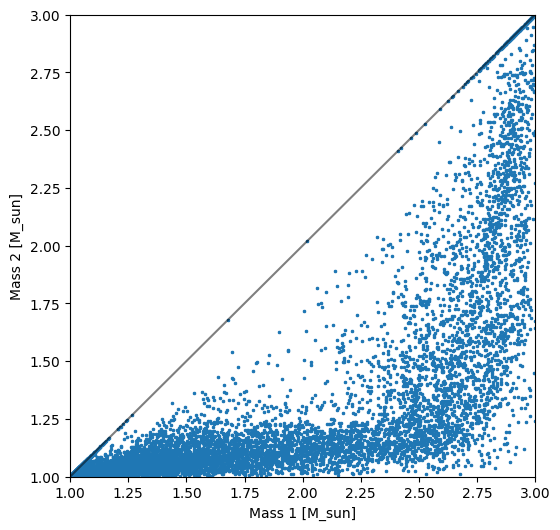
\includegraphics[width=\textwidth]{images/ew/template_bank_mass1_mass2.png}
    \caption{}
    \label{fig:ew_tb_mass1_mass2}
\end{figure}
%
\begin{figure}
    \centering
    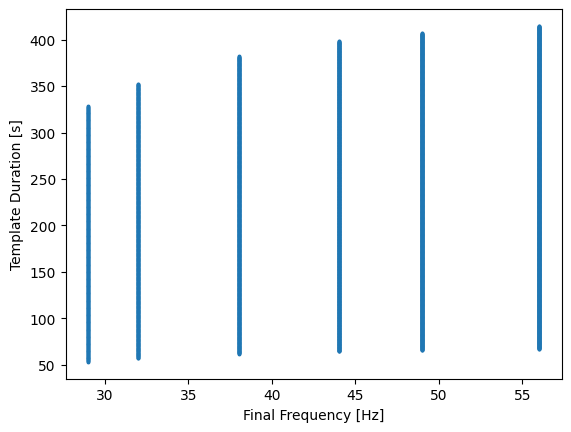
\includegraphics[width=\textwidth]{images/ew/template_bank_ffinal_duration.png}
    \caption{}
    \label{fig:ew_tb_duration_ffinal}
\end{figure}
%
The template bank distribution in mass 1 and mass2 can be seen in figure~\ref{fig:ew_tb_mass1_mass2} and the template duration and final frequency of the templates in the bank can be seen in figure~\ref{fig:ew_tb_duration_ffinal}.

\section{Event Localisation}

(BRILLIANT PAGE FOR THIS https://emfollow.docs.ligo.org/userguide/early\_warning.html)

We have previously mentioned the ability for the early warning search to provide a preliminary sky map of an event to aid in localisation pre-merger when passing information to the wider scientific community for followup in the multi-messenger regime. To demonstrate the sky map localisation as the signal progresses through our template bank we can perform a test using a representative $1.4M_\odot$-$1.4M_\odot$ BNS signal at a random point on the sky, and a few different distances, and evaluate the sky maps produced by BAYESTAR.

We produce the $1.4M_\odot$-$1.4M_\odot$ BNS signal and scale the distance so that it will be seen by the early warning search with SNRs: $10$, $20$, $30$. Then we search for these signals with the early warning search and for each candidate produced by the search we look at the sky map and the number of \verb|degrees|$^2$ in the 50\% credible area to see how the signal becomes more localised as more of the signal is being seen. We plot injection as a star on the sky maps and the $50\%$ confidence interval contours are plotted for each final frequency event belonging to the same injection on the same sky map, these can be seen in figure~\ref{fig:ew_10SNR_multiple} for the 10 SNR injection, figure~\ref{fig:ew_20SNR_multiple} for the 20 SNR injection and, figure~\ref{fig:ew_30SNR_multiple} for the 30 SNR injection. A table has also been produced containing the sky localisation area for each final frequency event for each of the injections, table~\ref{tab:ew_inj_skymaps}.
%
\begin{figure}
    \centering
    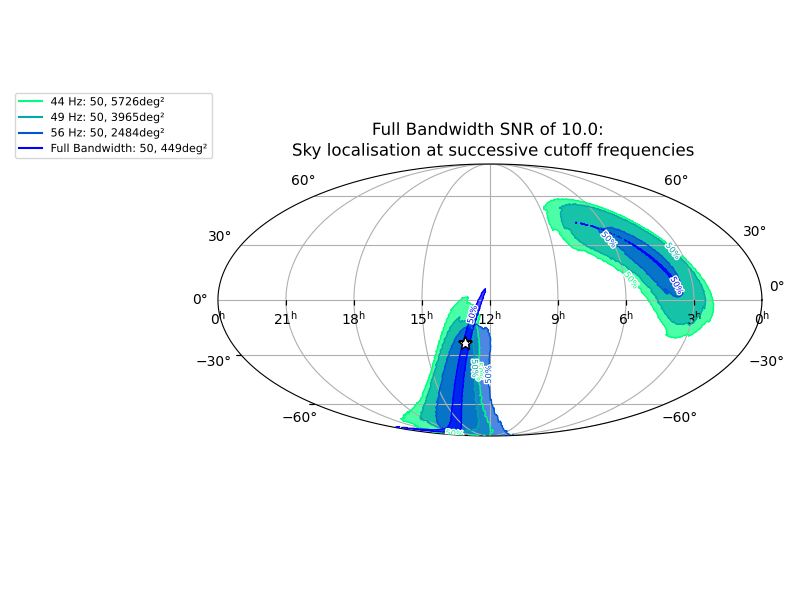
\includegraphics[width=\textwidth]{images/ew/10SNR_multiple.png}
    \caption{}
    \label{fig:ew_10SNR_multiple}
\end{figure}
%
\begin{figure}
    \centering
    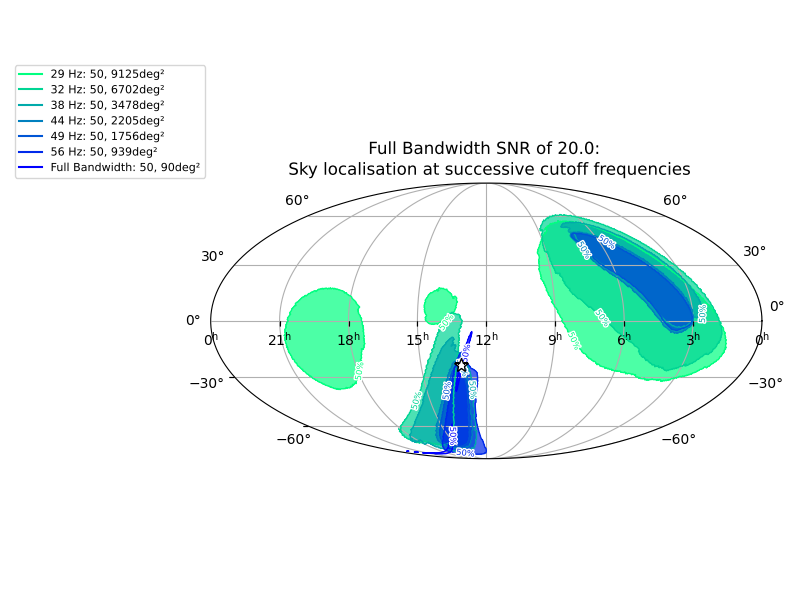
\includegraphics[width=\textwidth]{images/ew/20SNR_multiple.png}
    \caption{}
    \label{fig:ew_20SNR_multiple}
\end{figure}
%
\begin{figure}
    \centering
    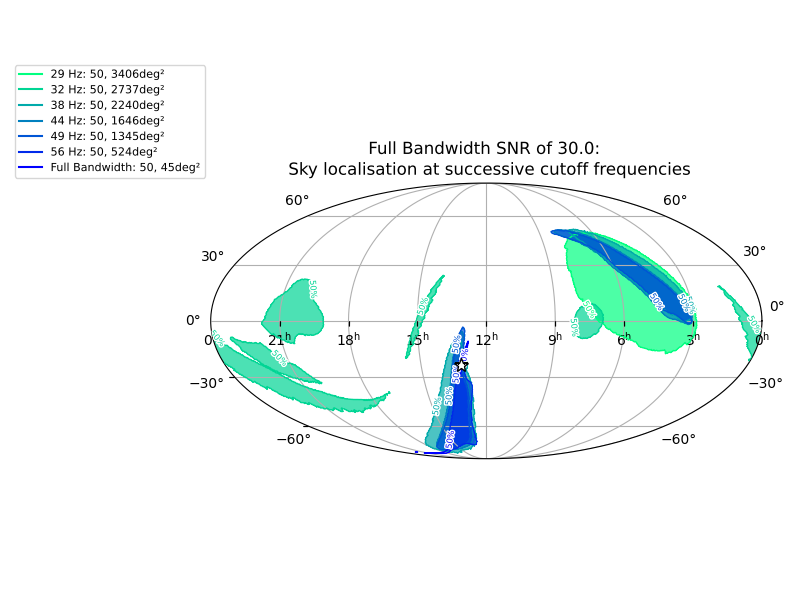
\includegraphics[width=\textwidth]{images/ew/30SNR_multiple.png}
    \caption{}
    \label{fig:ew_30SNR_multiple}
\end{figure}
%
\begin{table}[h!]
    \centering
    \begin{tabular}{|l|c|c|c|}
        \hline
        \textbf{Final SNR} & \textbf{10} & \textbf{20} & \textbf{30} \\ \hline
        \textbf{Sky map} & 
        Figure~\ref{fig:ew_10SNR_multiple} &
        Figure~\ref{fig:ew_20SNR_multiple} &
        Figure~\ref{fig:ew_30SNR_multiple} \\ \hline
        \textbf{Frequency} & \multicolumn{3}{|c|}{\textbf{Localization accuracy} (50\% credible area)} \\ \hline
        29 Hz & Not detected    & 9125 deg$^2$ & 3406 deg$^2$ \\ \hline
        32 Hz &  & 6702 deg$^2$ & 2737 deg$^2$ \\ \hline
        38 Hz &  & 3478 deg$^2$ & 2240 deg$^2$ \\ \hline
        44 Hz & 5726 deg$^2$ & 2205 deg$^2$ & 1646 deg$^2$ \\ \hline
        49 Hz & 3965 deg$^2$ & 1756 deg$^2$ & 1345 deg$^2$ \\ \hline
        56 Hz & 2484 deg$^2$ & 939 deg$^2$  & 524 deg$^2$ \\ \hline
        1024 Hz & 449 deg$^2$ & 90 deg$^2$   & 45 deg$^2$ \\ \hline
    \end{tabular}
    \label{tab:ew_inj_skymaps}
    \caption{Table with Final SNR, Distance, Sky map, Frequency, and Localization accuracy (50\% credible area)}
\end{table}
%
It is the case, especially for the low SNR signal, that the injection at every final frequency cutoff. Figure~\ref{fig:ew_10SNR_multiple} is missing the \verb|29, 32| and \verb|38| Hz events. It is very clear to see in table~\ref{tab:ew_inj_skymaps} that a higher SNR directly translates to a better sky localisation. The 30 SNR injection has been constrained sky maps at all frequencies.

DESCRIBE THE SKY MAPS AND THE CONTOUR INTERVALS. 50\% REFERS TO THE SMALLEST AREA ON THE SKY, MINIMIZED. FIND OUT HOW THIS IS DONE. 

\section{Existing Limitations}

\subsection{Computational Limitations}

The early warning search is heavily optimized to the point it runs on a single dedicated machine with $10$ processes and $2$ threads per process. Just as the with full bandwidth search, the template bank is parallelised over these processes using MPI so each process will be performing the matched filter for only a few hundred templates before the message passing interface receives all the results and the coicidences are found by the rank 0 process. The search can be badly affected by other processes running on the same machines so this machine is exclusively used by the PyCBC Live early warning search.

The search can suffer heavily from other non-PyCBC processes such as file storage, data frame delivery or GraceDB uploads. These can be mitigated slightly with reserved local storage on the dedicated machine or subprocess multiprocessing for the GraceDB uploads so the search isn't waiting on GraceDB to continue processing, especially at times where multiple events are being uploaded for a single signal and across multiple searches from other pipelines.

Another consideration and computational limitation is the limit in introducing new computationally complex processes to the search that might introduce lag to individual processes. Potential changes to the ranking statistic could be challenging to implement without slowing down individual processes or the coincidence rank 0 process. With a data stride of one second we need to be sure that the data processing for the current second is completed before the next second of data arrives or we will slowly build up a debt of data which the search can never get on top of.

\subsection{Physical Limitations}

The template bank does not include any spins on the templates thereby neglecting any effects on the waveform or from precession, however, it is unlikely to see precession at such low frequencies due to the effect becoming more pronounced over increasing numbers of orbits.

Electromagnetically bright events are very rare in the LVK regime, as of May 2024 only (NUMBER) out of (TOTAL NUMBER) events are within our template bank range, and of those only (NUMBER) have been observed with electromagnetic counterparts.

\section{Injection Runs in Offline}

To investigate the efficacy of the early warning search I performed an injection campaign very similar to the injection campaigns done in the previous chapters, (ARCHENEMY), (PYCBCLIVE). This time using an injection set I generated myself to include exclusively signals that should be seen by the early warning search, as opposed to the premade rates and populations injection sets.

\subsection{Injection Set \& Data}

The injection set contains 32604 unique injections placed every ~100 seconds, encompassing 3456000 seconds or exactly 40 days worth of data. The parameters which vary by injection and the ranges in which they vary can be seen in table~\ref{tab:ew_inj_params}.
%
\begin{table}[h]
    \centering
    \begin{tabular}{|>{\raggedright}p{3cm}|>{\raggedright}p{5cm}|>{\raggedright\arraybackslash}p{5cm}|}
        \hline
        \multicolumn{3}{|c|}{\textbf{Variable Parameters}} \\
        \hline
        \textbf{Parameter} & \textbf{Value Range} & \textbf{Prior Distribution} \\ \hline
        mass1 & 1.0 - 3.0 & uniform \\ \hline
        mass2 & 1.0 - 3.0 & uniform \\ \hline
        spin1z & -0.05 - 0.05 & uniform \\ \hline
        spin2z & -0.05 - 0.05 & uniform \\ \hline
        distance & 10 - 1000 & uniform radius \\ \hline
        coa\_phase & - & uniform angle \\ \hline
        inclination & - & sin angle \\ \hline
        polarization & - & uniform angle \\ \hline
        ra & - & uniform sky \\ \hline
        dec & - & uniform sky \\ \hline
        \hline
        \multicolumn{3}{|c|}{\textbf{Static Parameters}} \\
        \hline
        \textbf{Parameter} & \textbf{Value} & \textbf{} \\ \hline
        approximant & IMRPhenomXAS & \\ \hline
        f\_lower & 17 & \\ \hline
        f\_ref & 17 & \\ \hline
    \end{tabular}
    \caption{Parameters and their priors}
    \label{tab:ew_inj_params}
\end{table}
%
These injections are made into simulated noise with no non-Gaussian artefacts or non-stationarity and a constant PSD. The distances generated for each injection are re-scaled after the initial injection set has been created to ensure a uniform SNR distribution of the signals between 12 and 60. Therefore the distances might not be exactly uniform in radius and the injection set should be thought to be distributed uniformly in SNR instead.

\subsection{Results}

Each injection has the potential to be seen by six different templates and therefore we might expect to see exactly six times the number of injections in the data. However, for the very low final frequency templates in the bank (29Hz) these would require at least 4 (DOUBLE CHECK) SNR (the SNR threshold for detection) to be accumulated in a very small frequency window, which is very unlikely for the 12 SNR injections but possible for our 60 SNR injections. (CHECK THIS TO SEE WHAT THEY ACTUALLY FOLLOW, MINIMUM SNR FOR 29Hz DETECTION)

Another reduction in the number of candidates found will be caused by a very short time gap between final frequencies 49Hz and 56Hz. The evolution of the gravitational wave signals inspiral increases over time and therefore these two frequencies might be found within a stride and therefore one will be skipped. These two effects will cause a reduction in the total number of candidates seen by this injection test.

The total number of candidates found for all injections is (NUMBER). 

PyCBC Live outputs the candidates found during the search and outputs the time of coalescence of the non-truncated template. Therefore, even if a 29Hz template finishes many seconds before time of coalescence of the gravitational wave signal, we can collect all of the candidates associated with an injection by comparing injection time and time of coalescence of candidates. We look for candidates with a time of coalescence within +-0.5 seconds of the injection time, this ensures that we are looking for candidates which have all been predicted to end in the same search stride.

Figure~(REF) shows a histogram of the number of candidates found per injection. (INSERT THE FIGURE)

\section{Identified Problems}

The purpose of performing this experiment is to see where the early warning search is lacking and could be improved in the future to allow for greater chance of properly detecting these exceedingly rare events when they occur for real.

We have identified some problems with the early warning search during this injection test which we will describe here, where possible I will indicate whether these problems can be solved as of right now or if more work needs to go into developing solutions in the PyCBC Live search. Alongside this, some of these problems are expected and the solutions would harm the search and so are left as is.

\subsection{Candidates across search boundaries}
%
\begin{figure}
       \centering
    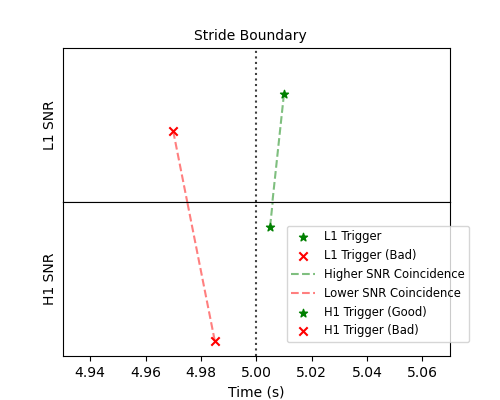
\includegraphics[width=\textwidth]{images/ew/cands_across_bounds.png}
    \caption{}
    \label{fig:ew_boundary_candidates_trig_plot}
\end{figure}
%
The early warning search operates on a one second stride, meaning every single second the template bank is matched filtered with the data to discover any gravitational wave signals. In some cases the SNR of a template match filtered with the data will be above the SNR threshold in one second and again above the SNR threshold in the next second.

There are two scenarios for this case, the first second has a lower SNR than the following second: in this case, there will be two candidates uploaded to GraceDB with the same template and roughly the same time of coalescence (within 0.5 seconds) where one has a higher SNR than the other. We want to reduce the amount of lag from detection to upload so there is no possibilty of keeping a 'buffer' of candidates to hold whether a higher SNR candidate will occur in the next second and this will be a scenario that will just happen.

The second scenario is the same happening but the other way round, the first candidate has a higher SNR than the candidate in the following second. In this case we can happily upload the first candidate to GraceDB and then keep track of the uploaded candidates and prevent the upload of the second candidate if it has a lower SNR. This is already implemented in PyCBC Live for the single detector search and can be easily changed to be used for the early warning search too in the future.

In figure~\ref{fig:ew_boundary_candidates} you can see a great example of this happening for one of our injections. It appears that multiple candidates have been created for multiple final frequency templates, these candidates have different SNRs but are found with the same template and the same time of coalescence for the injection.
%
\begin{figure}
       \centering
    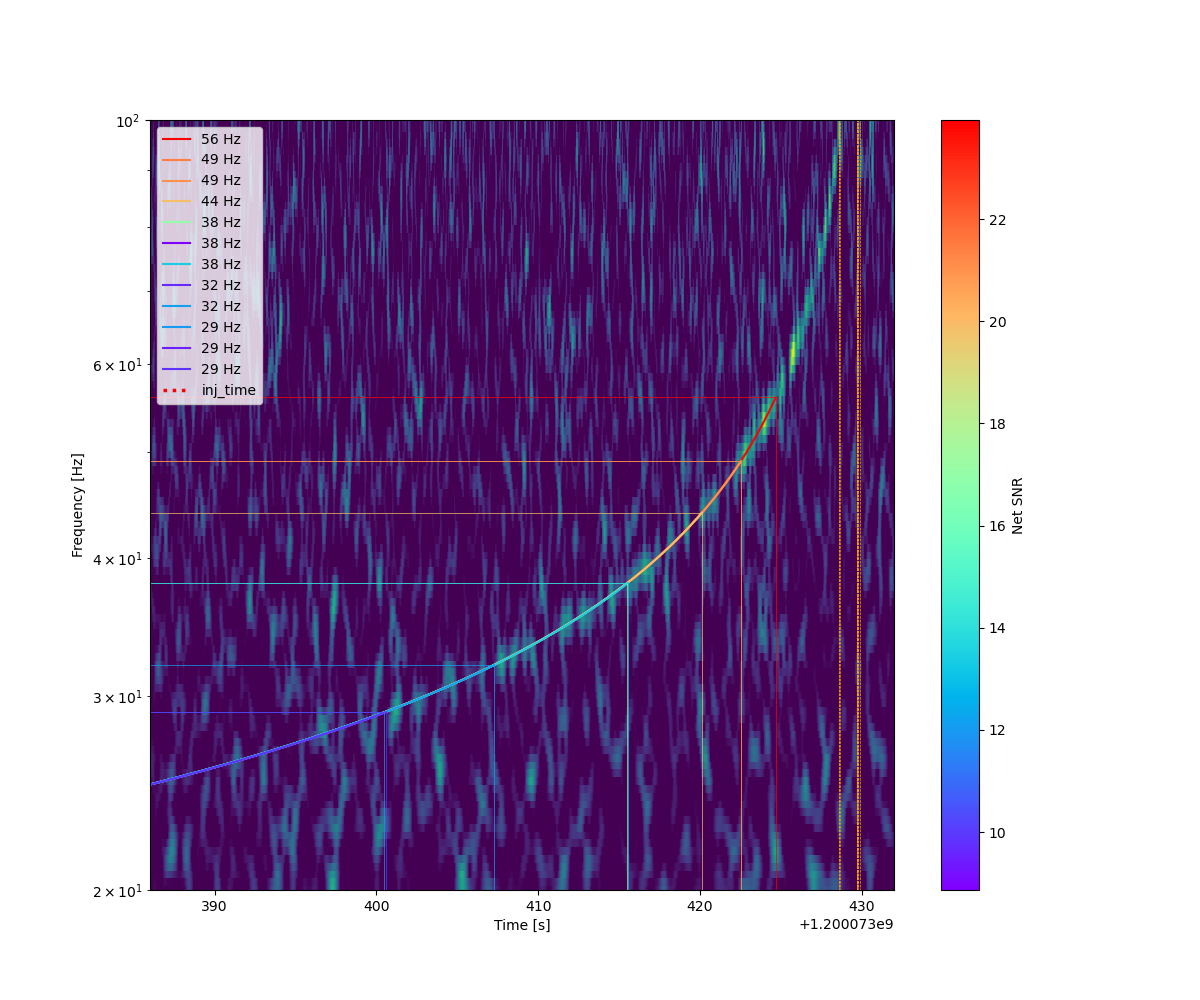
\includegraphics[width=\textwidth]{images/ew/multi_freq.png}
    \caption{}
    \label{fig:ew_boundary_candidates}
\end{figure}
%
\subsection{Triggers across search boundaries}
%
\begin{figure}
       \centering
    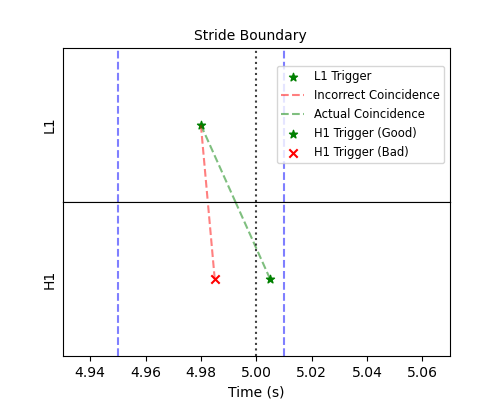
\includegraphics[width=\textwidth]{images/ew/trigs_across_bounds.png}
    \caption{}
    \label{fig:ew_trig_candidates_trig_plot}
\end{figure}
%
The early warning search operates using coincidences across detectors which have a phase-time consistency test included in the coincident detection ranking statistic. The time portion of this test allows for a light travel time (plus a small buffer) between triggers in different detectors. This light travel time can mean that triggers in separate detectors for the same gravitational wave injection can fall on different sides of a second stride. Therefore the early warning search will create two candidates with the highest SNR trigger in the first detector with two other triggers for the second detector in two separate second strides.

This is unfortunately unavoidable, we need the light travel time in the ranking statistic and this can straddle two strides. Tracking candidates uploaded in the previous second and holding an upload if the SNR is lower in the second second would still help but the same trigger from a single detector will be uploaded twice.

\subsection{Low significance candidates}

As with any search, the template bank can match on Gaussian noise in the data and produce low significance candidates that typically only upload a single candidate per injection. These can also end at a similar time of coalescence to another found injection and so can appear in the results as belonging to an injection when they are entirely independent and made of noise.

These can be treated by GraceDB in post-upload and disregarded quite quickly when further candidate uploads from higher final frequency templates have not been made. However, this is another consequence of the low-latency matched filter searches. Figure~\ref{fig:ew_same_tc} shows an example of an injection having another associated 29Hz candidate which ends at a similar time of coalescence but is on an entirely different track to the injection's other found candidates.
%
\begin{figure}
       \centering
    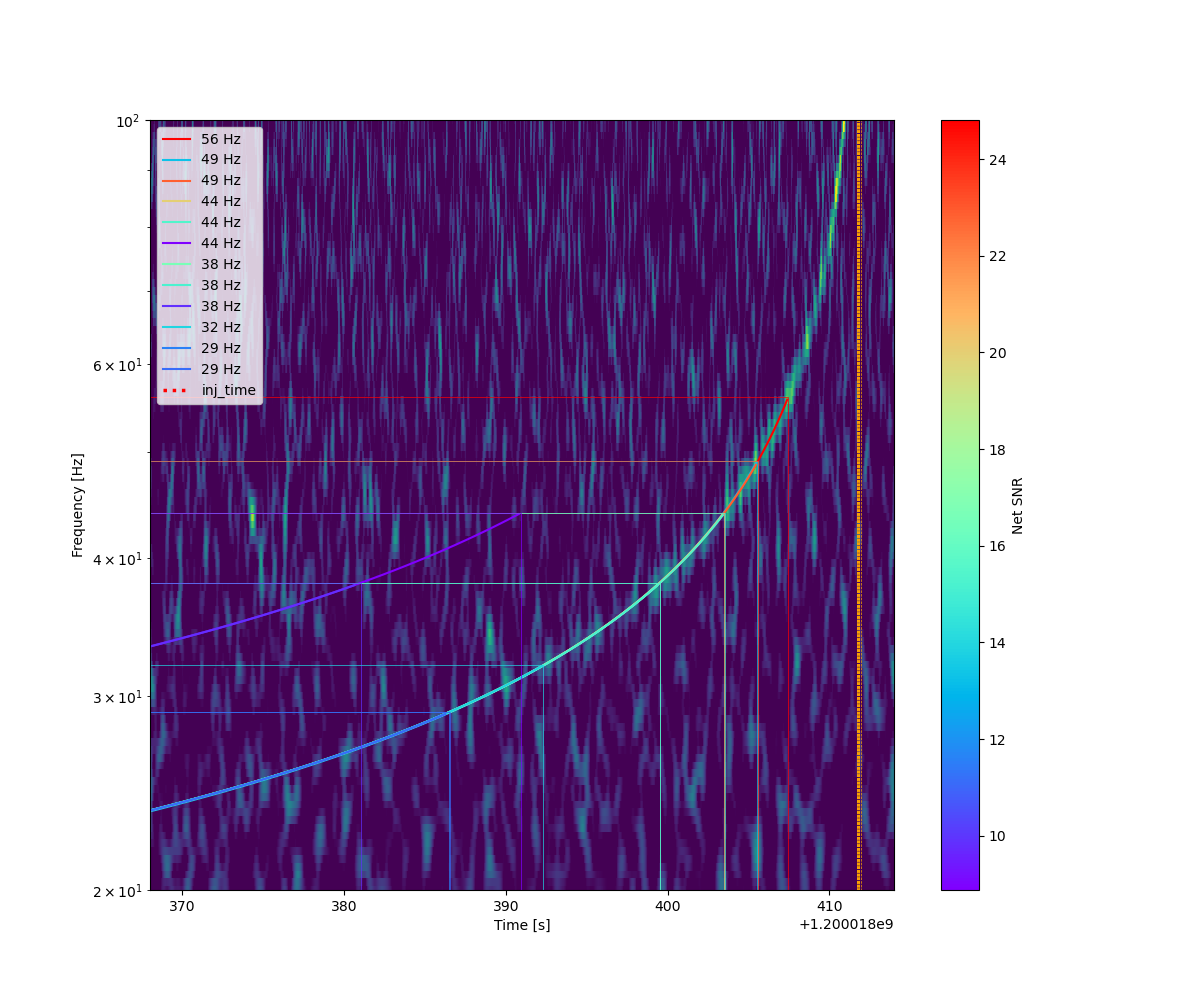
\includegraphics[width=\textwidth]{images/ew/same_tc.png}
    \caption{}
    \label{fig:ew_same_tc}
\end{figure}
%
\subsection{Non-monotonic SNR increases}

As a gravitational wave signal passes through the detectors we can match more and more of it to the gravitational wave template and can expect to see a higher and higher SNR. Therefore, for a specific gravitational wave signal we would expect an increasing SNR from each candidate corresponding to each final frequency in our template bank. We look at the network SNR from each candidate corresponding to a gravitational wave event and we can see if any consecutive candidates have a lower SNR from the previous candidate, an unexpected behaviour.

We find that 1398 injections have a non-monotonically increasing SNR at some point within their evolution. To prevent the effects of small noise fluctuations we compare the SNRs from the two candidates and assess whether there is a greater than 5\% drop in SNR. For example, if the 38Hz candidate has an SNR of 10, the 44Hz candidate must have an SNR of less than 9.5 to be counted as a non-monotonic injection.
%
\begin{figure}
       \centering
    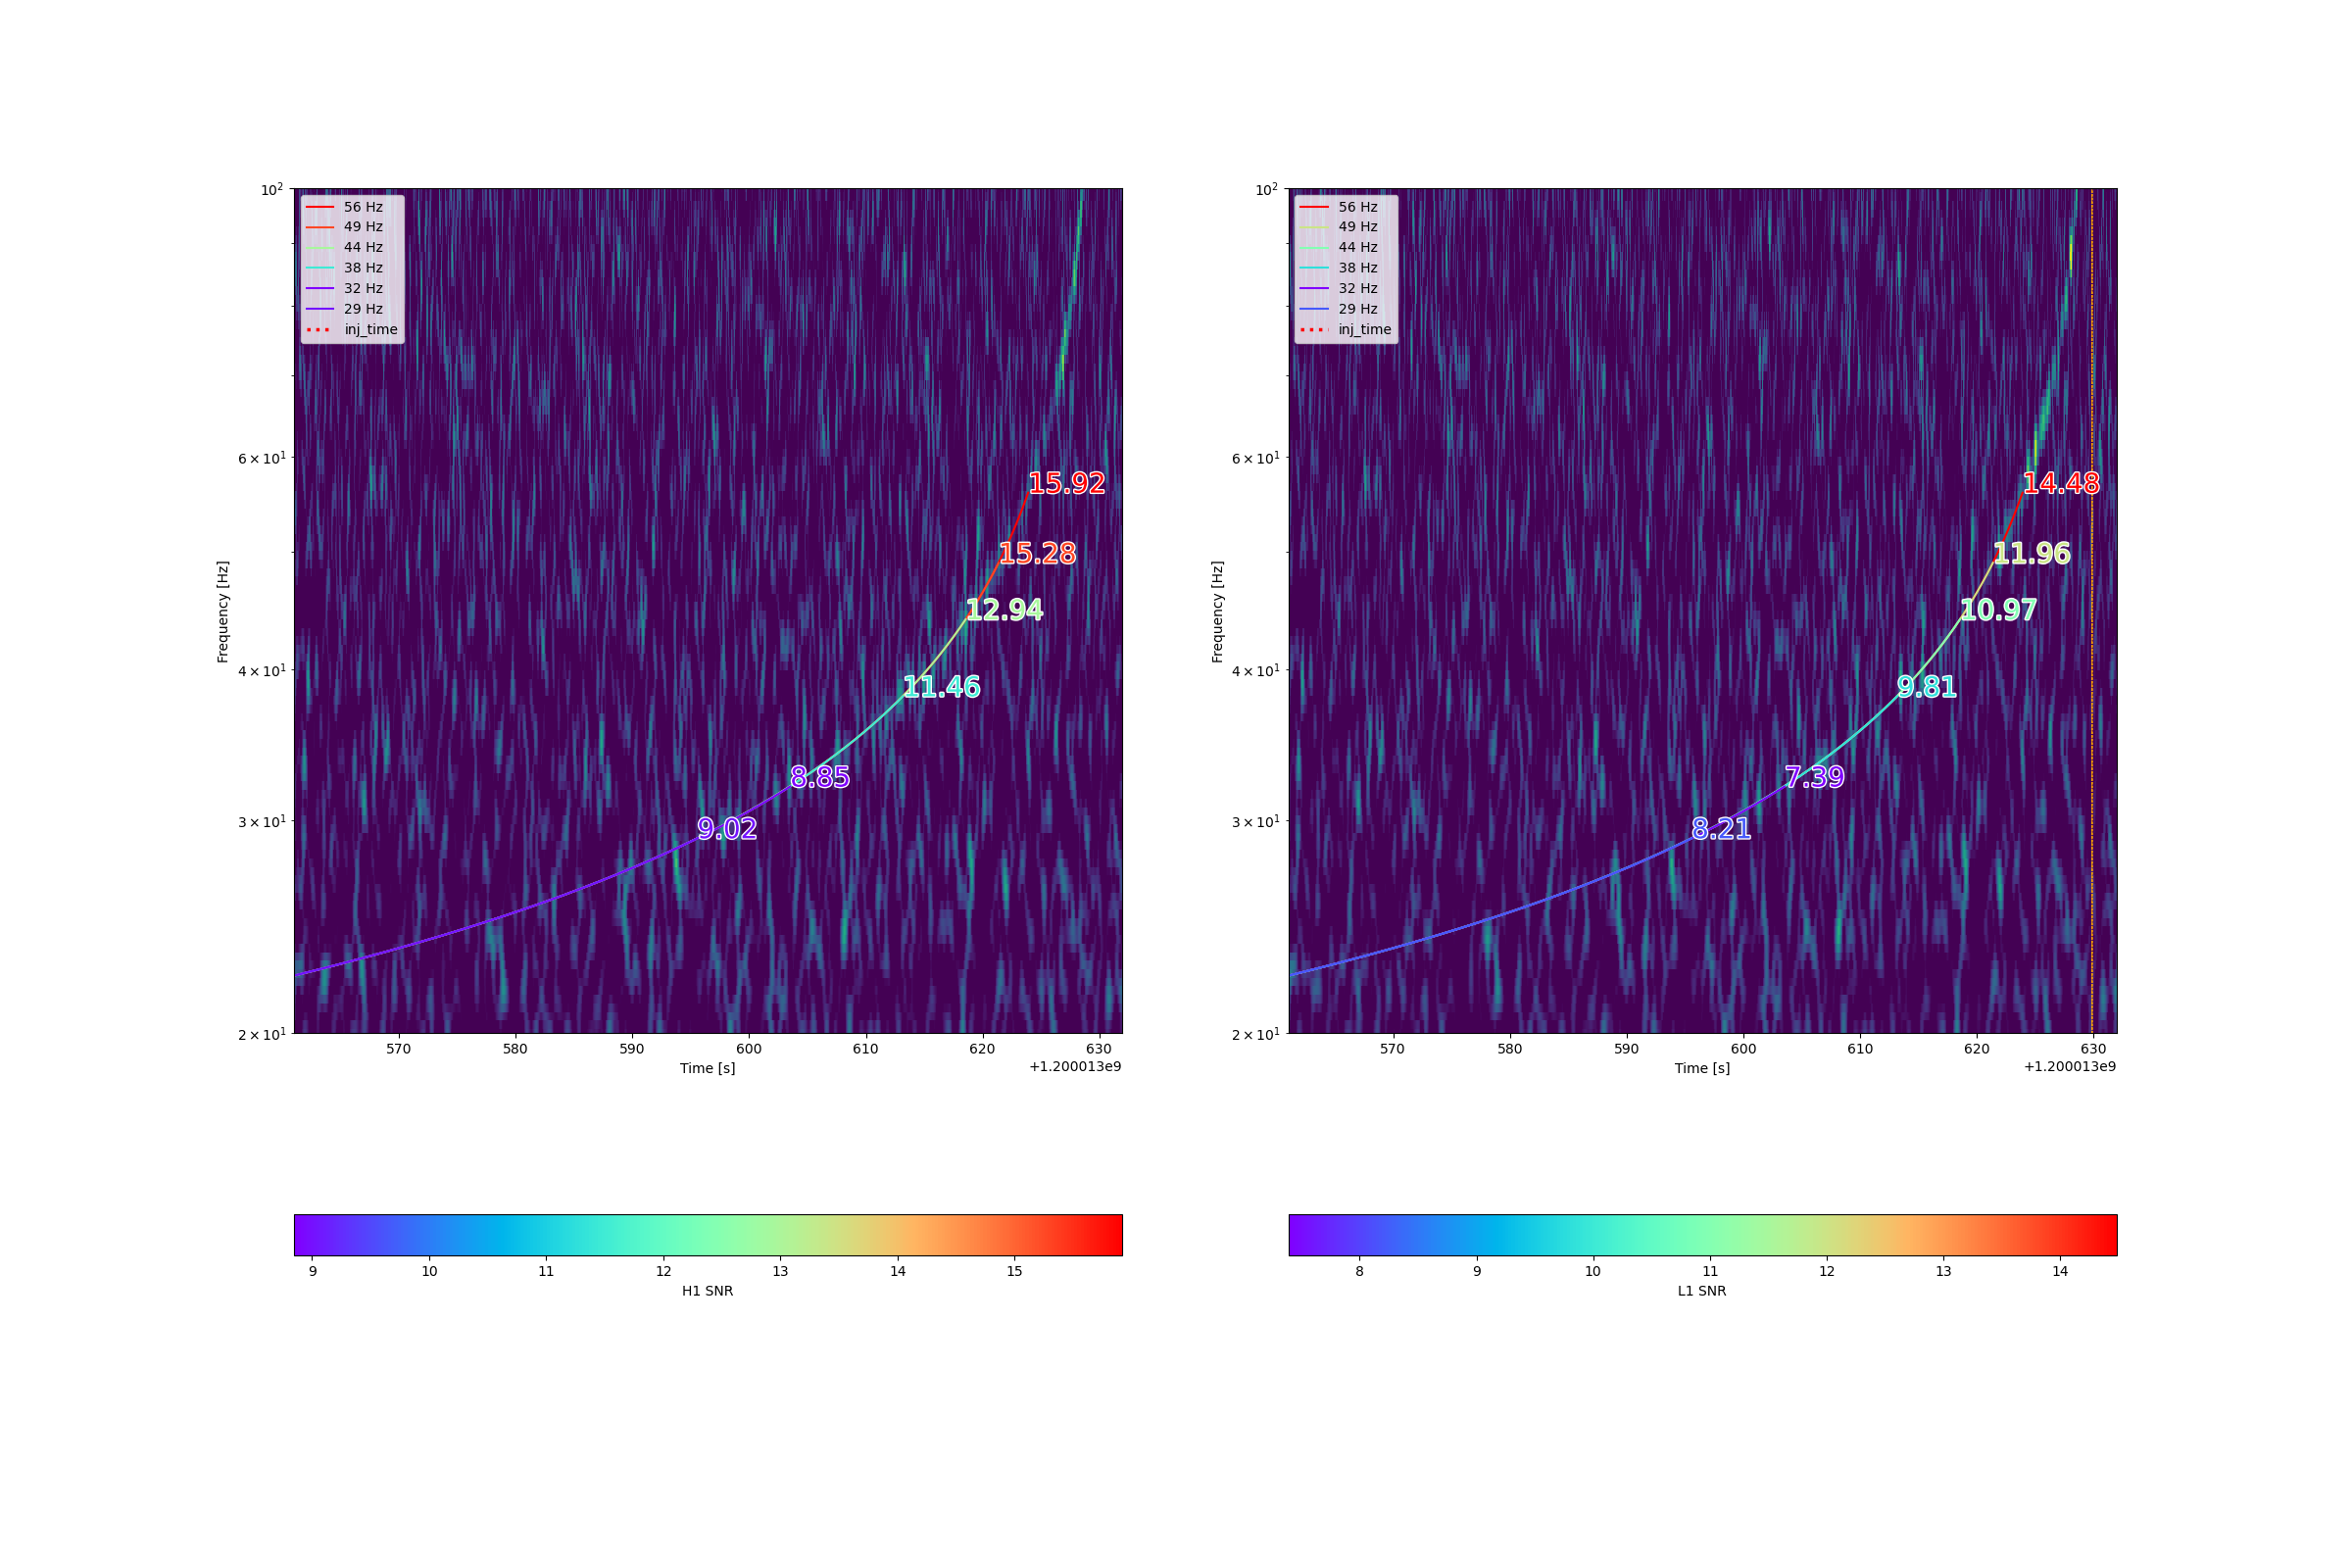
\includegraphics[width=\textwidth]{images/ew/small_non_monotonic.png}
    \caption{}
    \label{fig:ew_small_nonmono}
\end{figure}
%
\begin{figure}
       \centering
    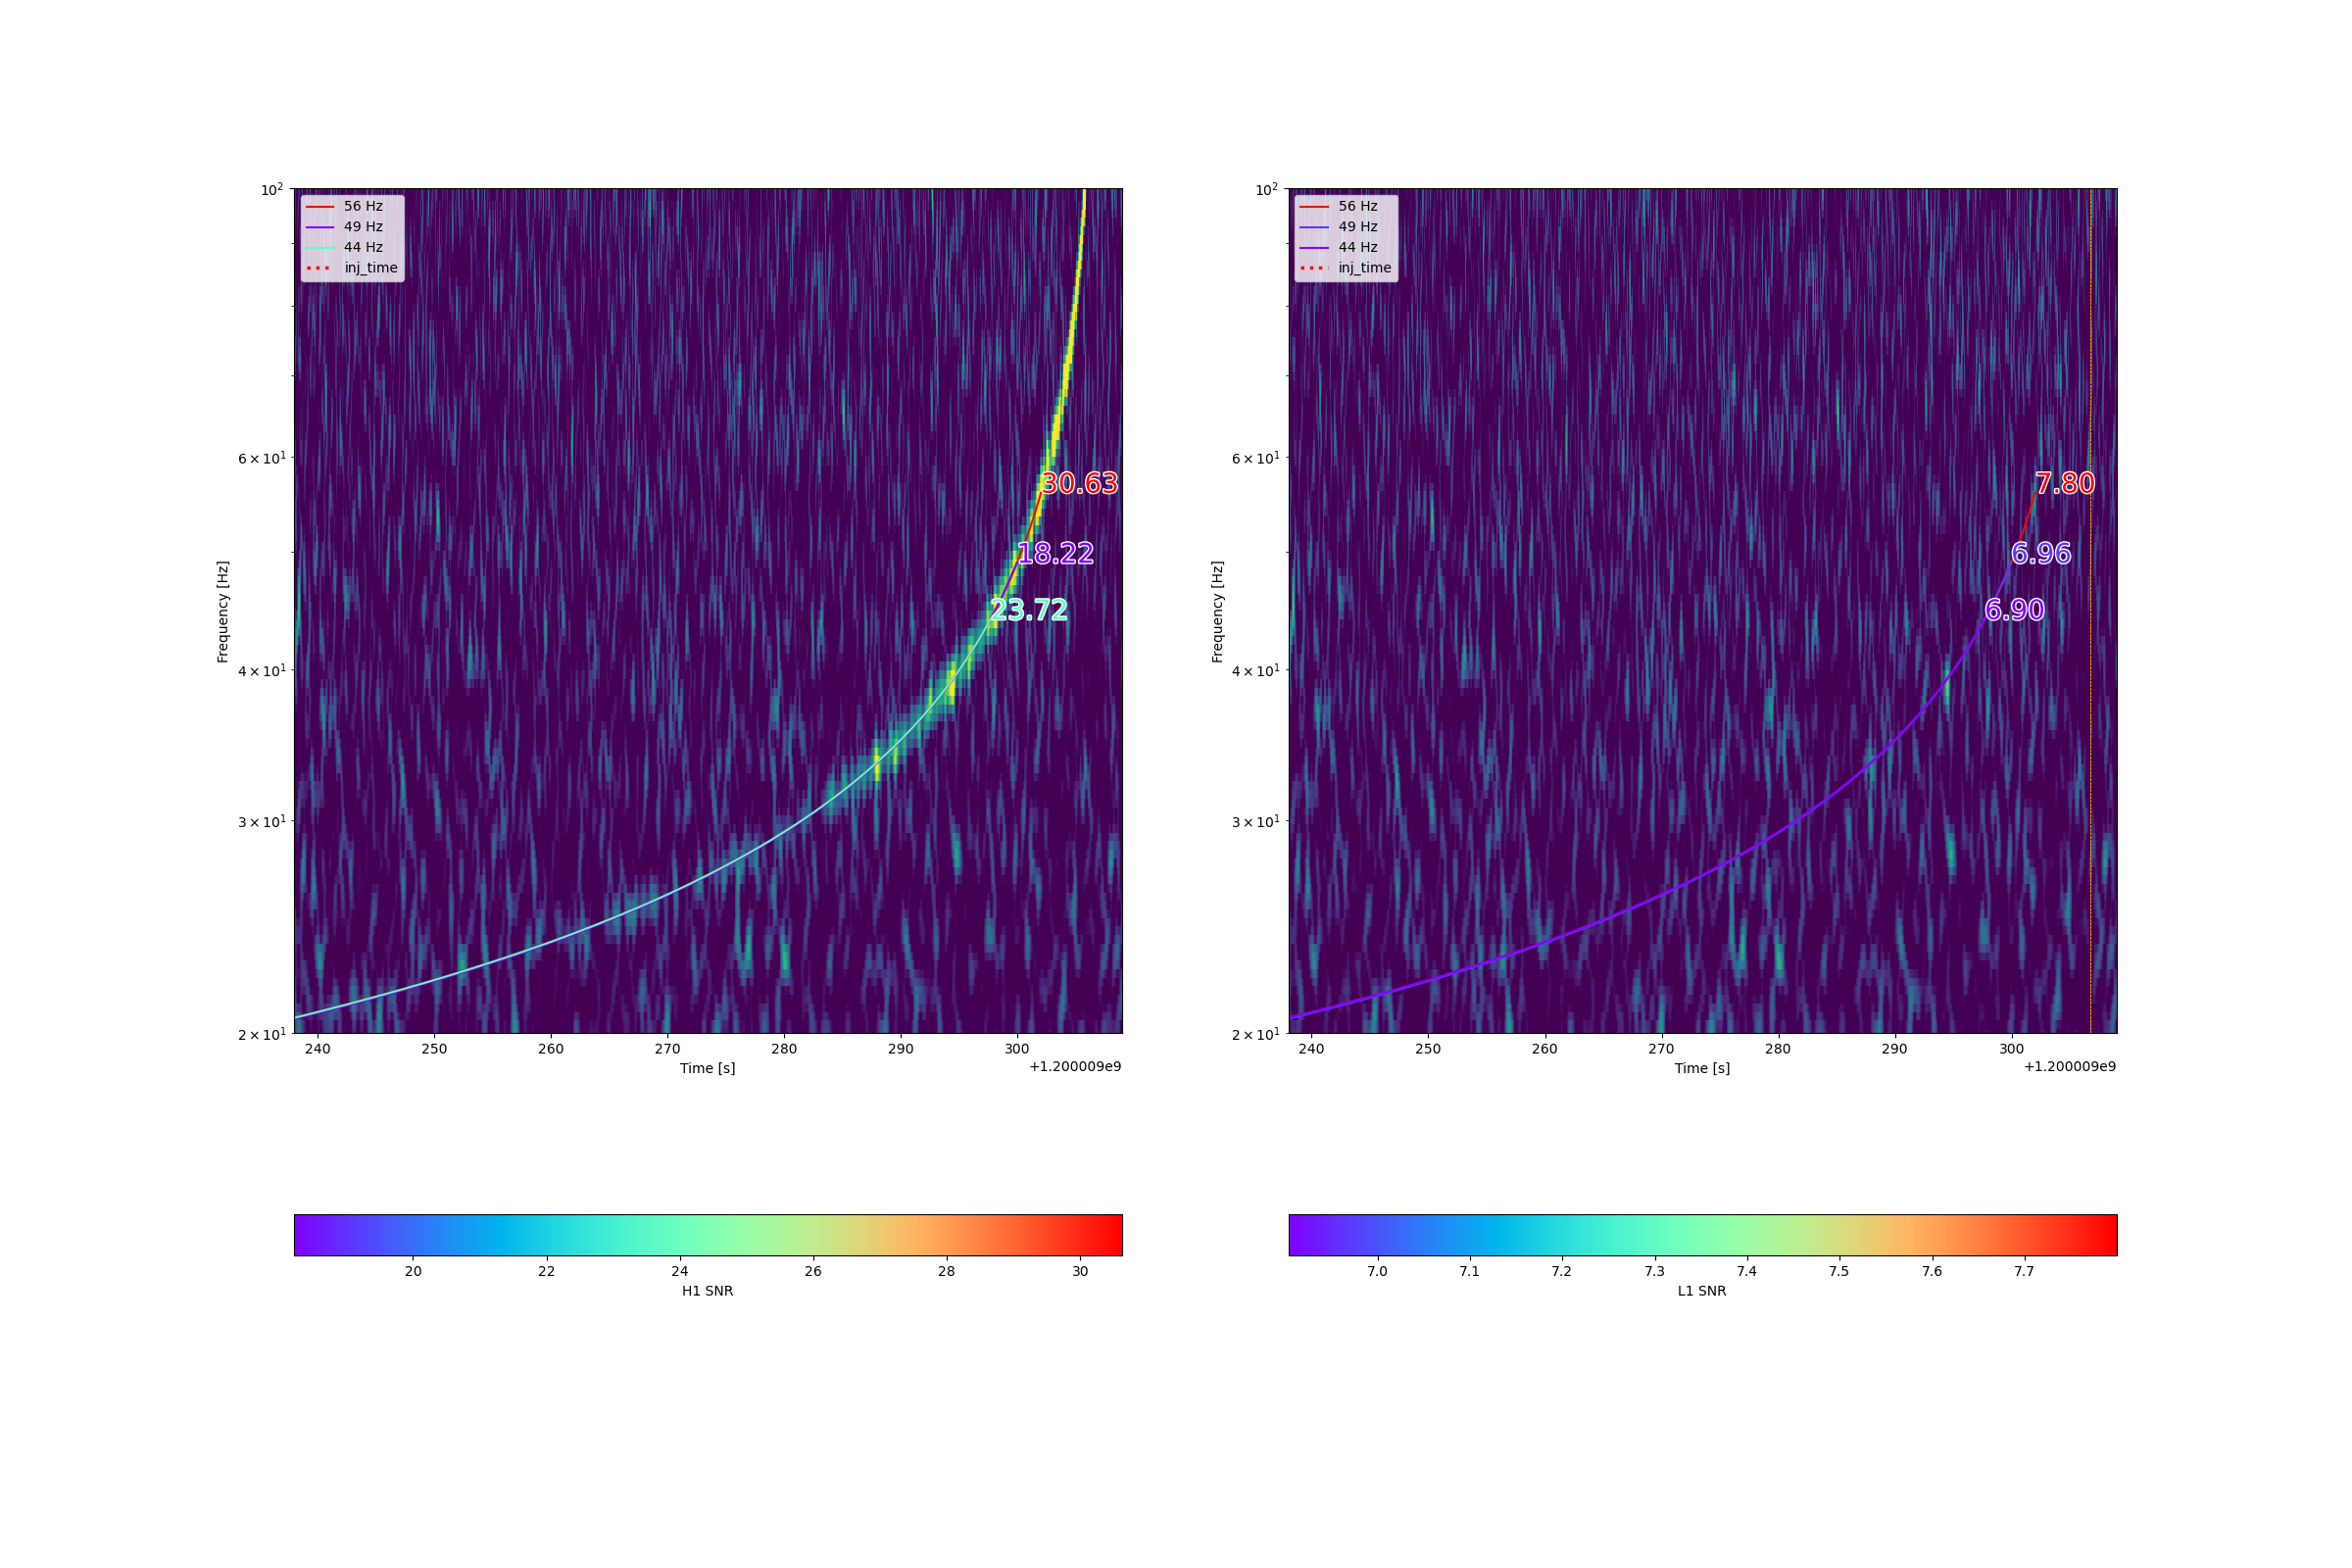
\includegraphics[width=\textwidth]{images/ew/large_non_monotonic.png}
    \caption{}
    \label{fig:ew_large_nonmono}
\end{figure}
%
To understand why these are happening, we have to look at the components that not only give us the SNR--the template and the data-- but also the ranking statistic, which might favour a slightly lower SNR template due to other properties of the noise. For example, the same template for the 38Hz and 44Hz candidates might give a monotonic increase in SNR but, a different template with a lower SNR for the 44Hz candidate might be more highly preferred event.

\subsection{Missing frequencies in signal evolution}

Injections which are missing frequencies are those that might seem to skip a frequency candidate, for example, progressing through from 32Hz to 38Hz, missing a 44Hz candidate and then finding a 49Hz and 56Hz candidate. We want to understand why the 44Hz candidate was missed. The smooth progression of frequency candidates could be used in the future as a measure of how real and event is, so to miss a candidate for a non-astrophysical reason might reduce our sensitivity.

There is a simple explanation for some events which is that the progression through to the higher frequencies might simple be too short for the search to identify a separate candidate. For the higher mass templates there might be few seconds between candidates. Others there is a clear problem and it is useful to understand why this has happened.
%
\begin{figure}
       \centering
    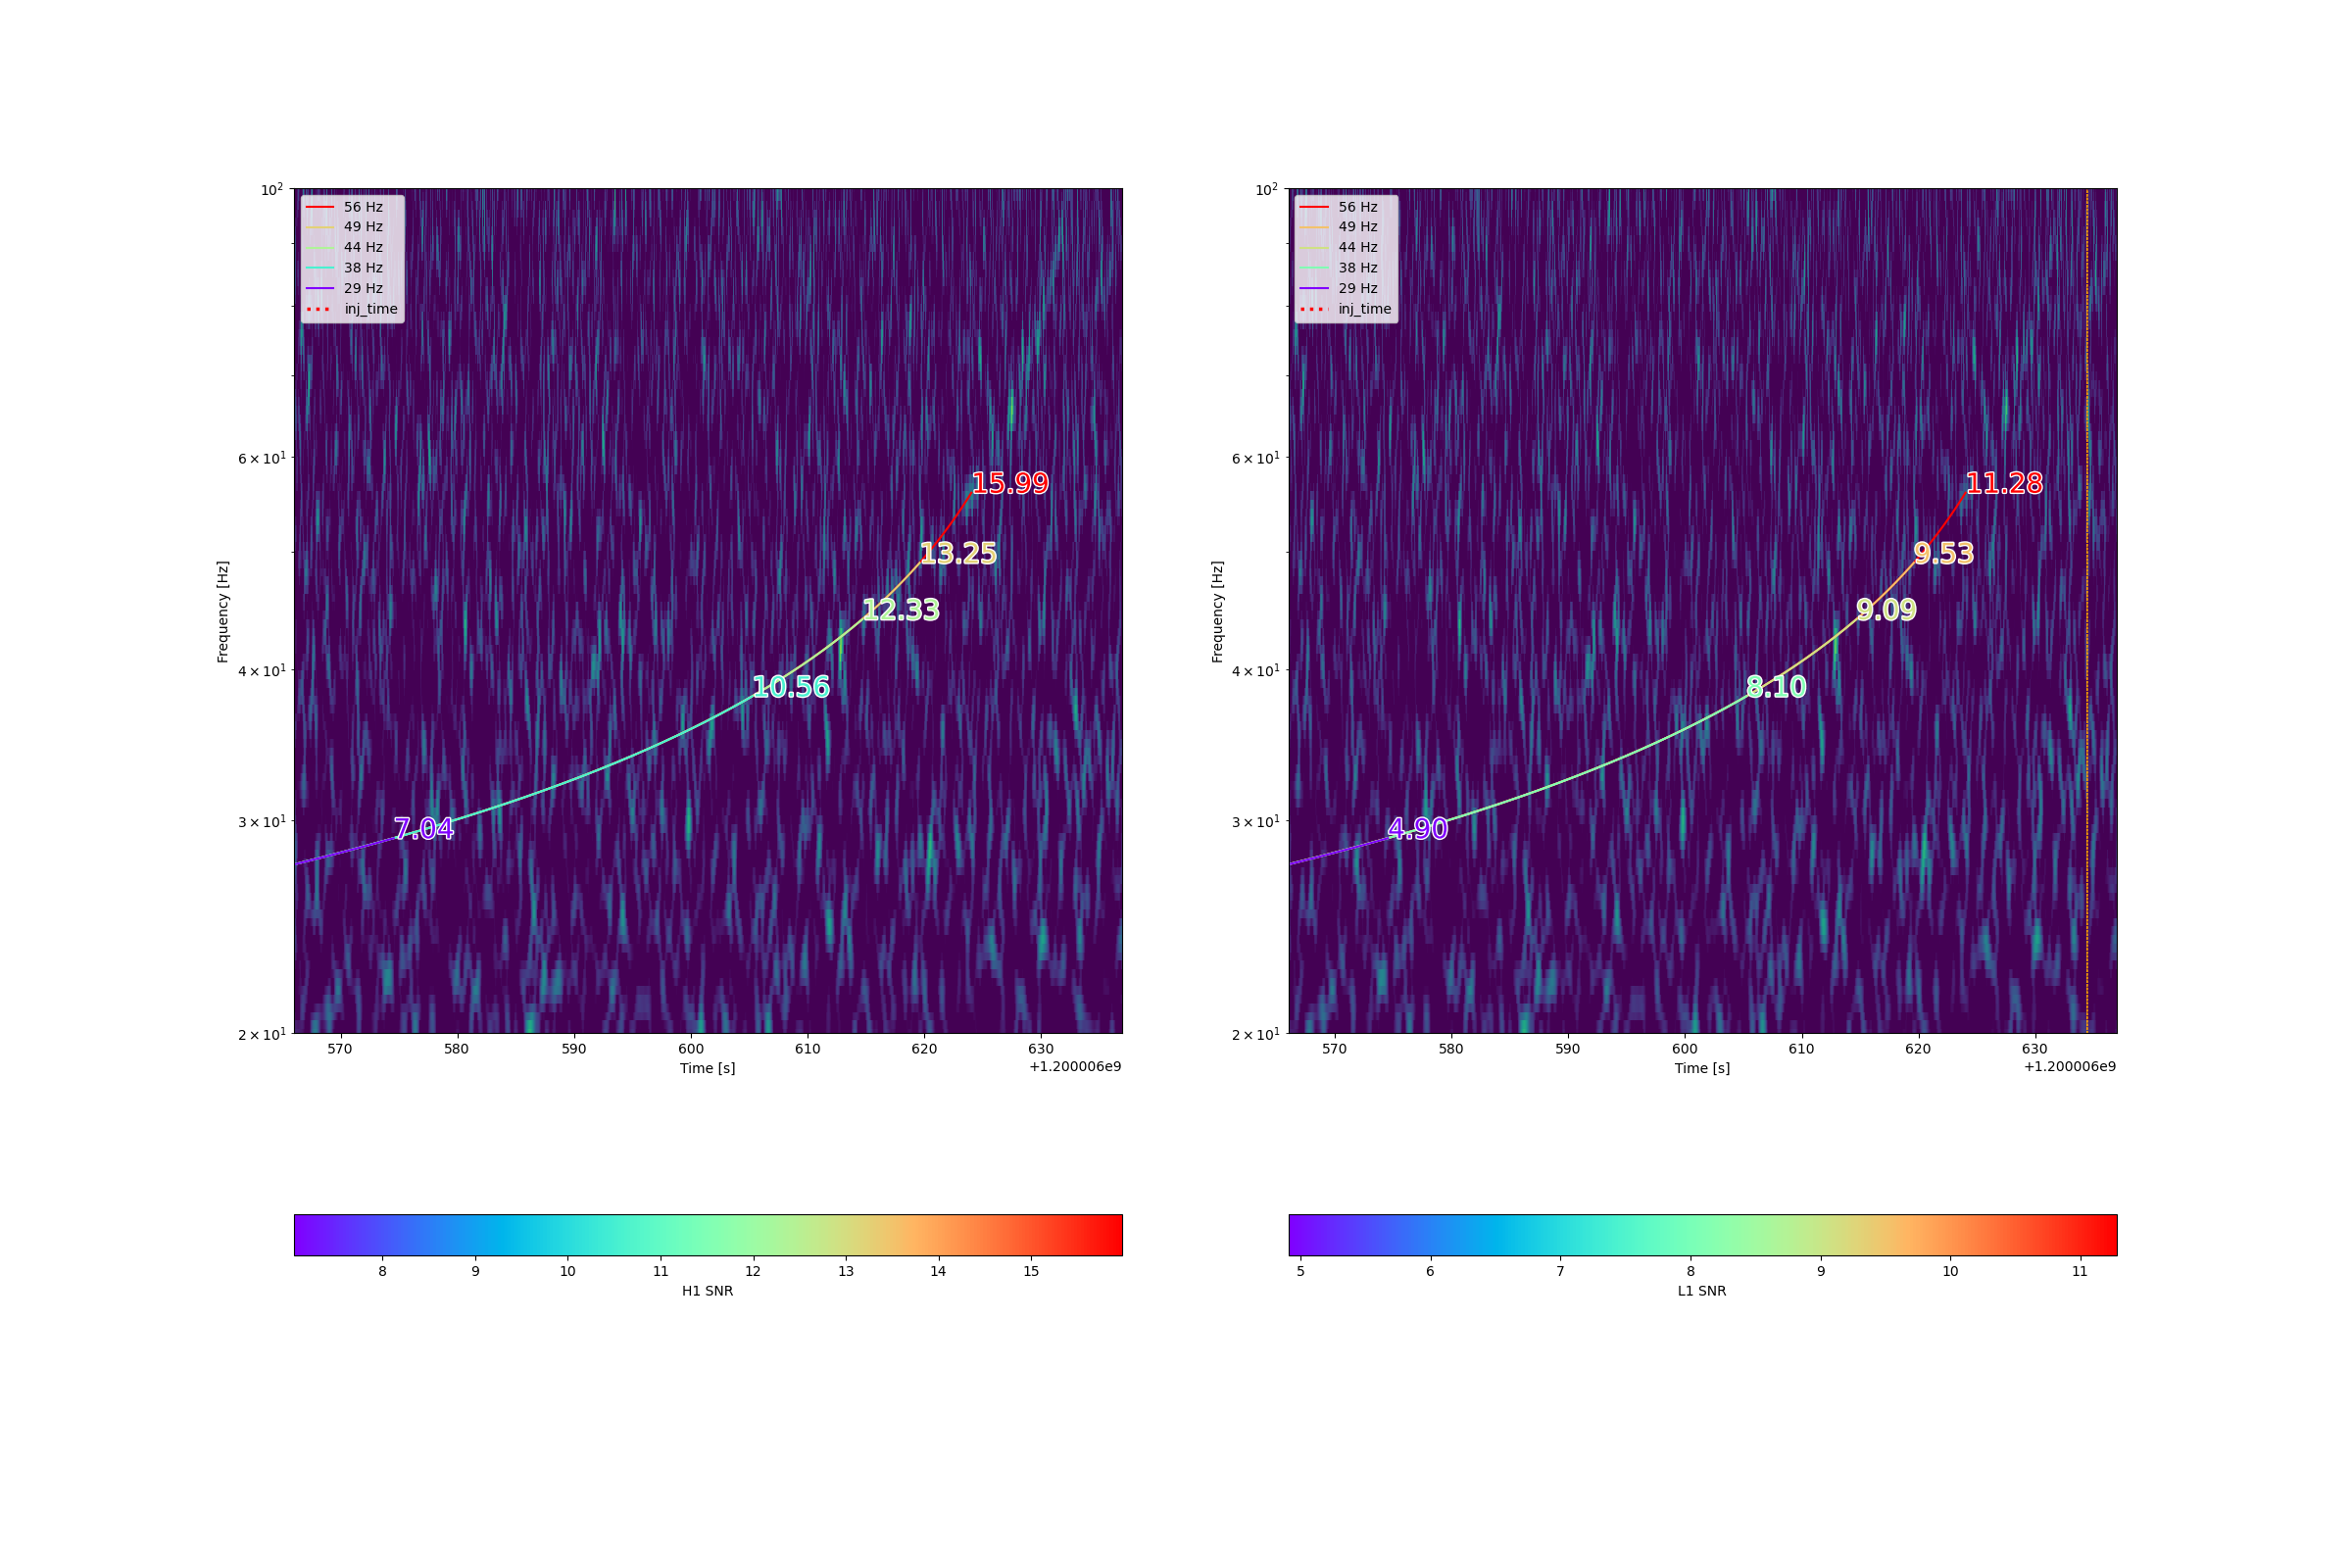
\includegraphics[width=\textwidth]{images/ew/Missing_freqs_1.png}
    \caption{}
    \label{fig:ew_missing_freqs1}
\end{figure}
%
\begin{figure}
       \centering
    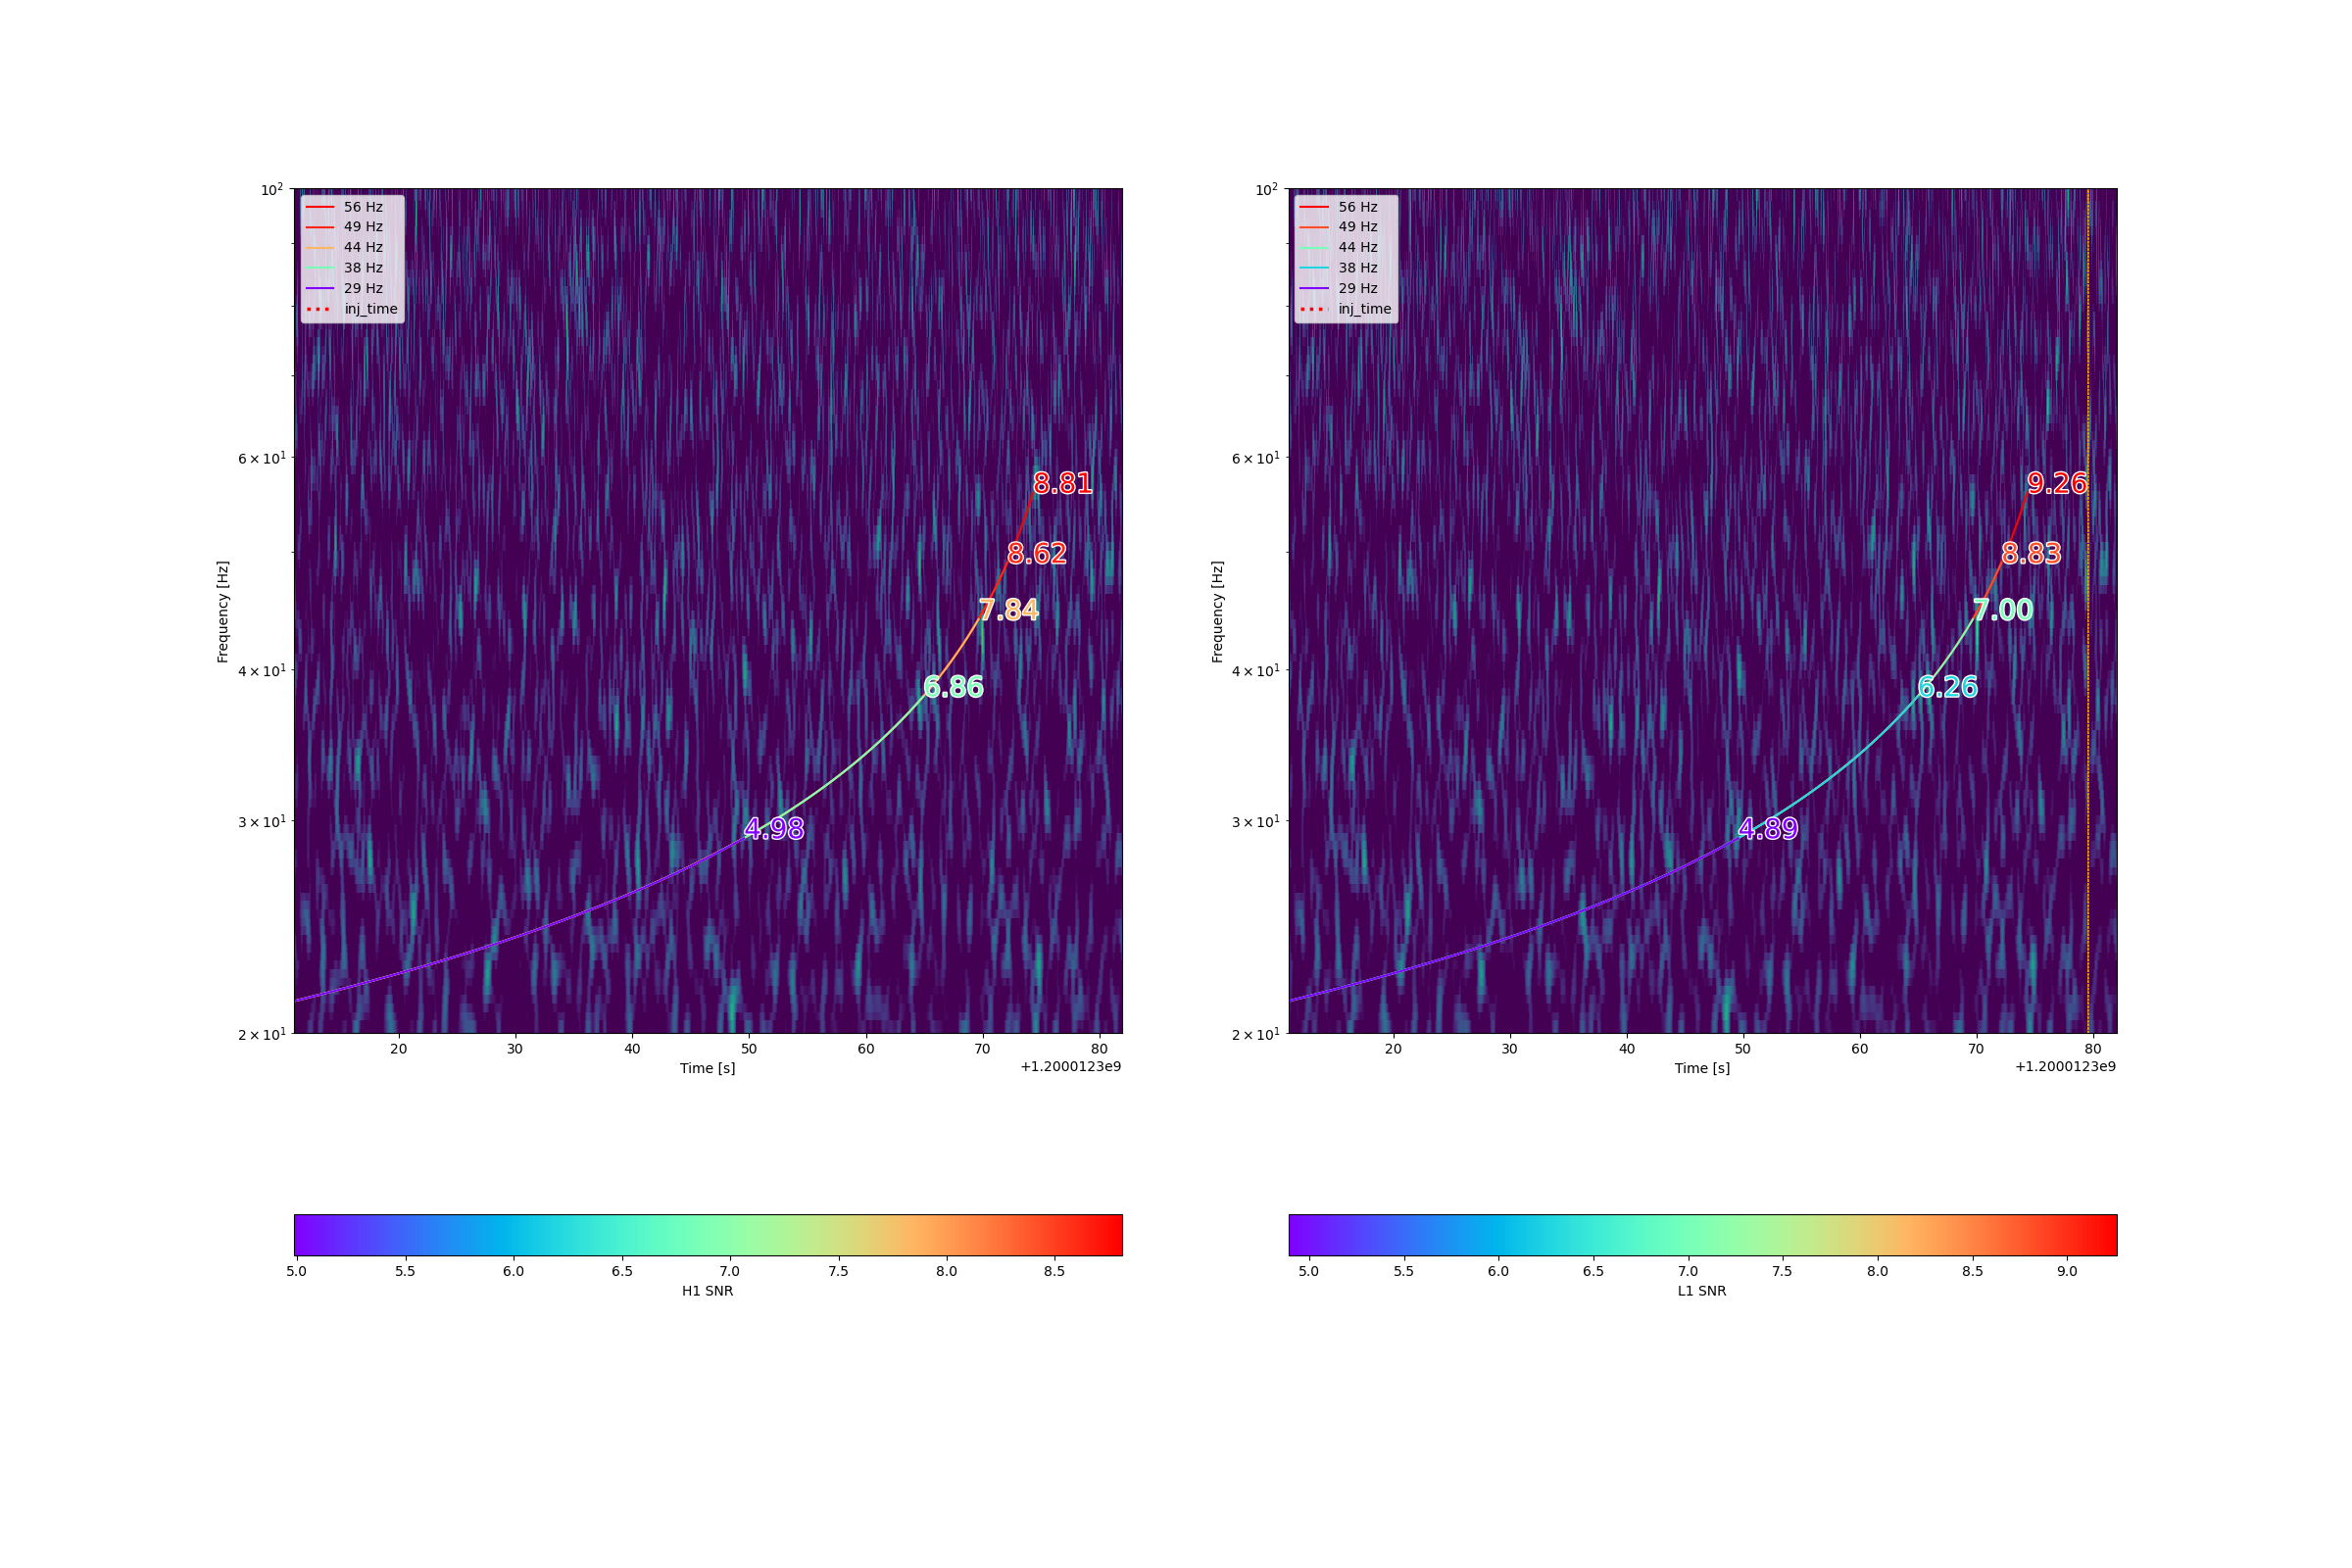
\includegraphics[width=\textwidth]{images/ew/missing_freqs.png}
    \caption{}
    \label{fig:ew_missing_freqs2}
\end{figure}
%
\subsection{Different templates found for one injection}

The lower frequency truncated templates have a higher degree of freedom to match with any incoming gravitational wave signal, as more SNR is accumulated when the gravitational wave is propagating through the detector the correct signal will be more and more apparent until merger. This means that we expect to see the template identified at each truncated frequency change slightly however, there is still a limit on this which we would like to understand.

If the template found by the 32Hz and 38Hz are in wildly different areas of the parameter space then we need to know why this has happened because the earlier we deliver a skymap to multi-messenger partners the better but, if we are delivering an incorrect skymap along with future frequency skymaps and skymaps from other searches then we risk confusing the telescopes and potentially losing a chunk of time in observation.

First we need to understand a limit in which we can accept a difference in template, we can evaluate this with a simple match between the consecutive templates or we could go further and study the skymaps that might be produced by the templates in the bank for the same injection and see how different they are.

We are not expecting the skymaps to vary too differently because the extrinsic parameters of the gravitational wave signal contribute more to the skymap and are less dependent on the template itself and more on the coincidence between the detectors, especially regarding the phase and amplitude seen by each detector which helps BAYESTAR to evaluate the contributions from the h+ and hx components of the gravitational wave and in a 3 detector regime can triangulate the source of the gravitational wave signal.

\subsection{Problems with Data}

One of the problems experienced while doing the data analysis of this project is an issue caused by the method of creating the data initially. The PyCBC function used was \emph{pycbc\_condition\_strain} which takes an input for the power spectrum density of the noise you with to simulate. We used an analytical PSD (NAME, REF, CITE) which produced discontinuities at the boundaries between our data segments and therefore negative effects on the matched filtering being performed by the live search. An example of one of these discontinuities and an injection missing some candidates can be seen in figure~\ref{fig:ew_boundary_problem}.
%
\begin{figure}
       \centering
    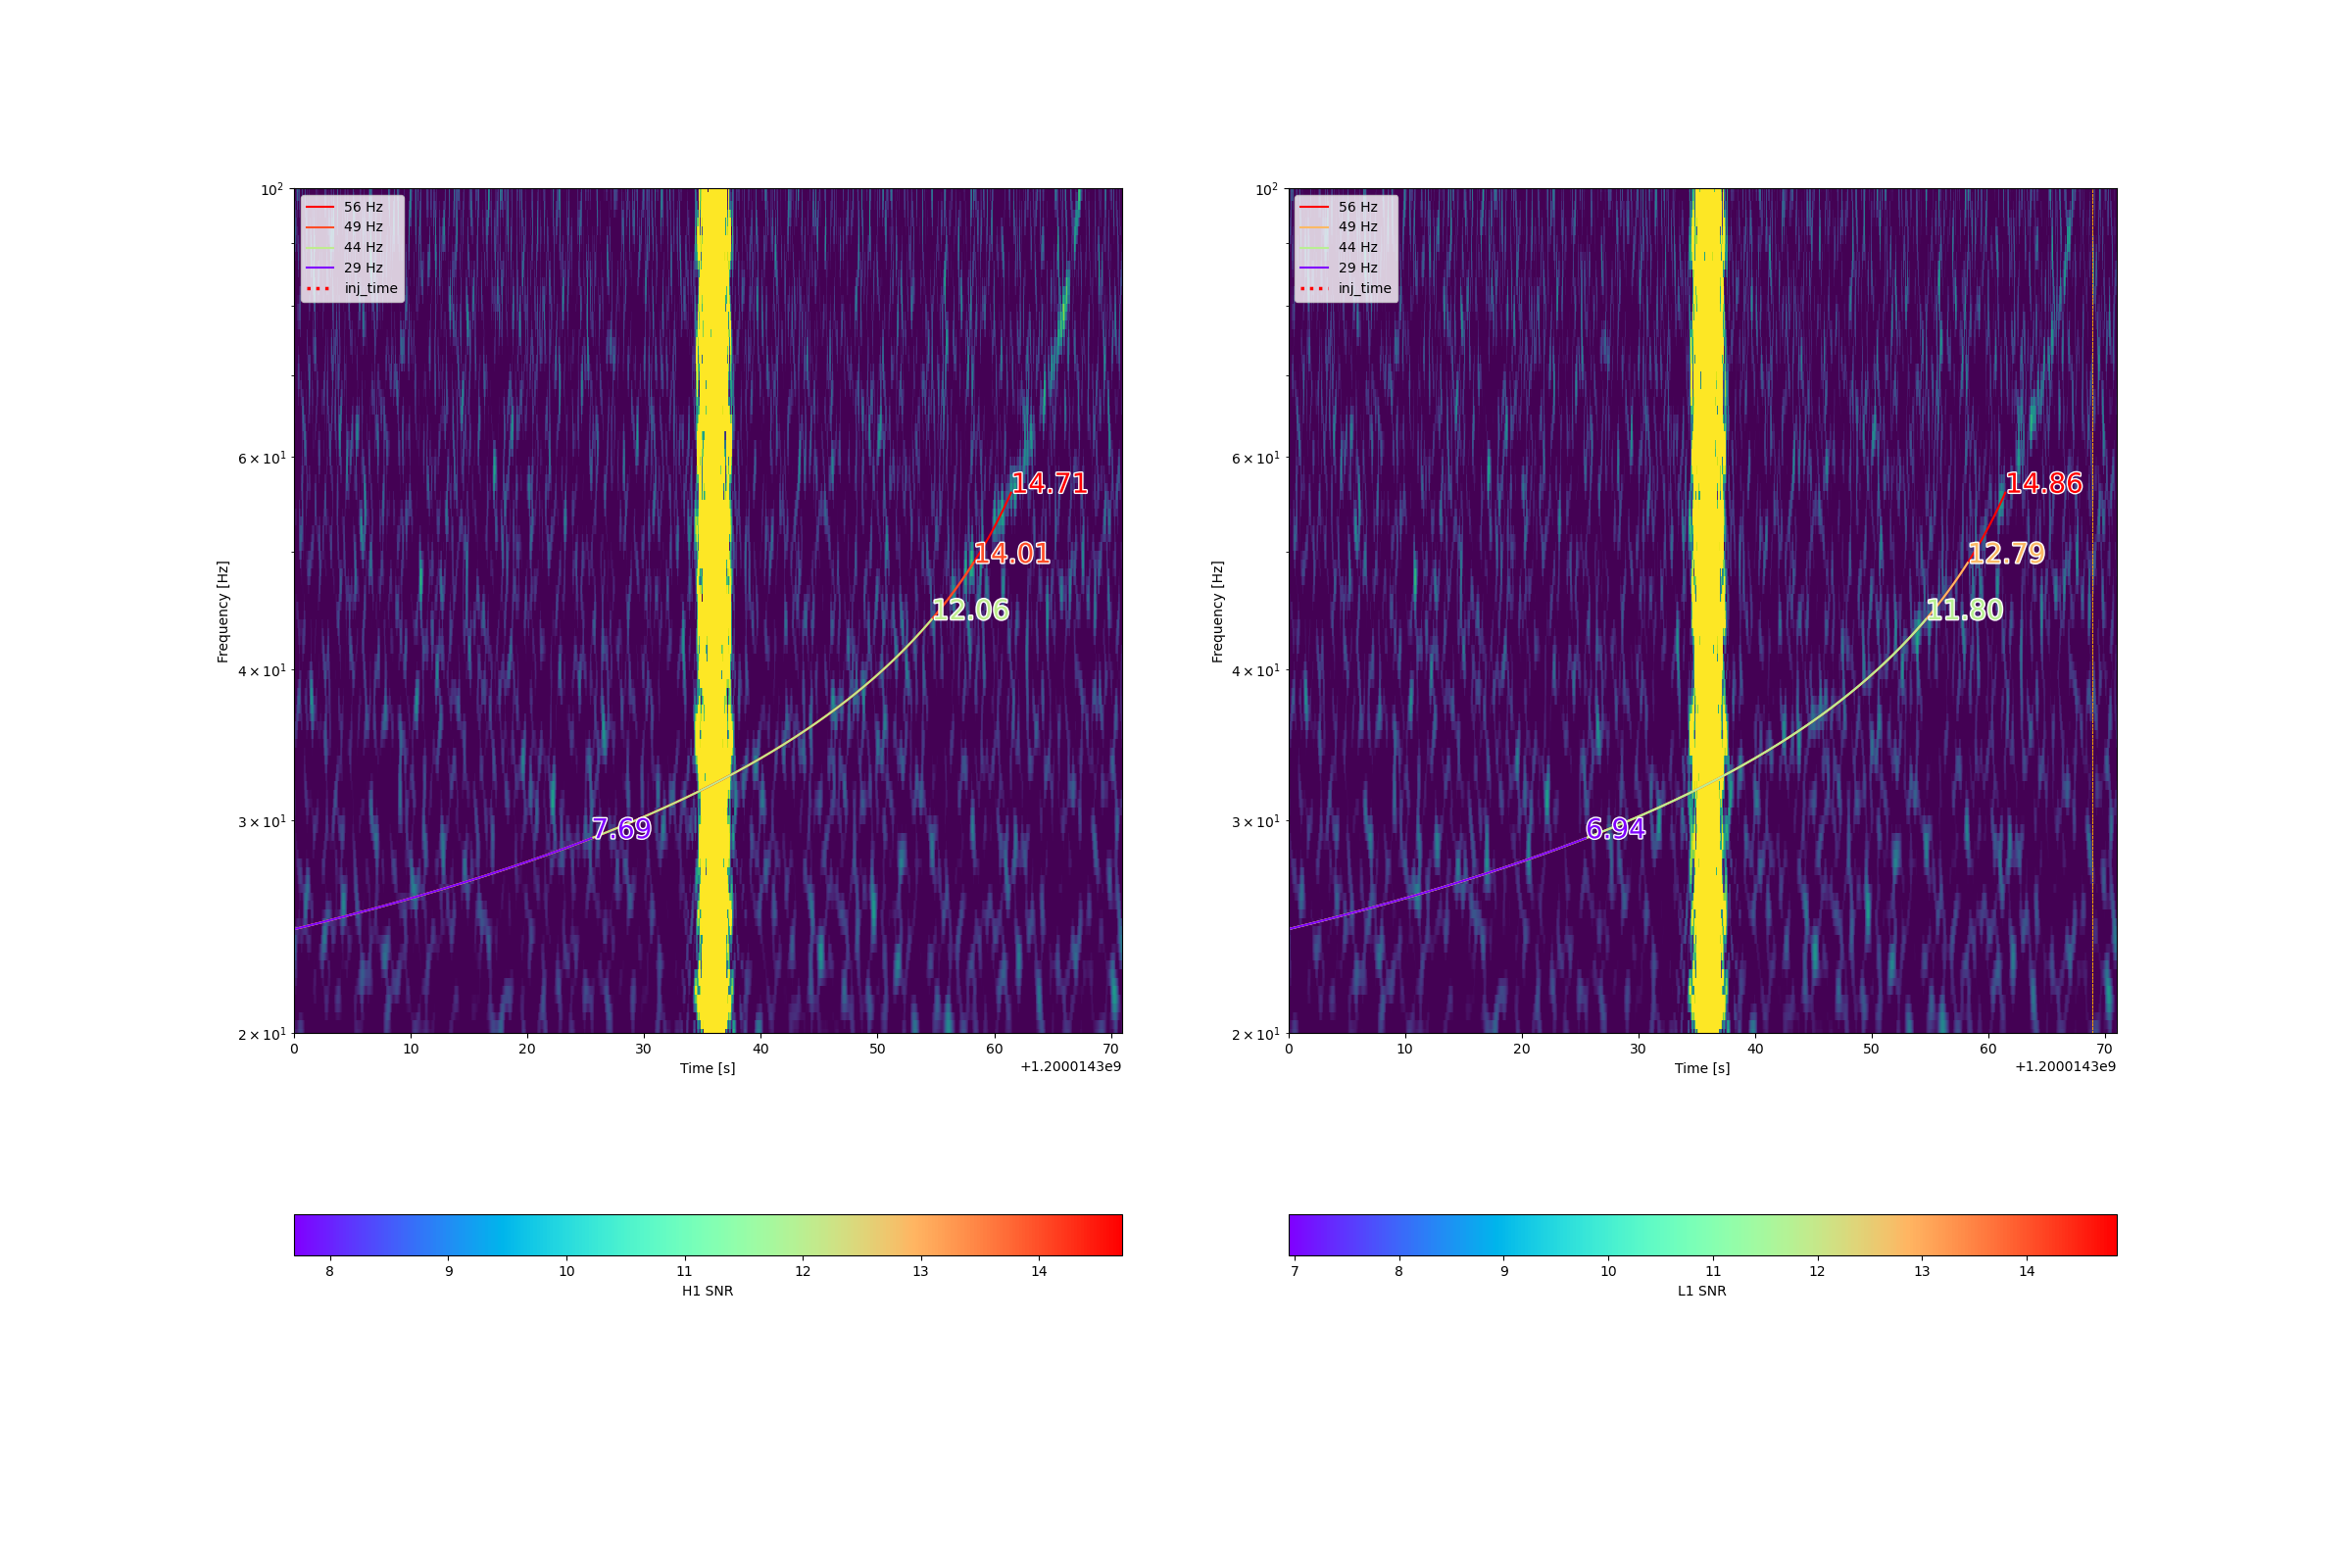
\includegraphics[width=\textwidth]{images/ew/injections_near_boundaries.png}
    \caption{}
    \label{fig:ew_boundary_problem}
\end{figure}
%
The bug can be explained by the analytical PSD not cutting off naturally when tending towards 0Hz and instead takes on values incompatible with a real PSD. This 'bug' has since been reported and a user-based solution has been found, to include a new argument to condition strain to perform a highpass on all frequencies below 10Hz. Unfortunately we did include a highpass argument on the data originall when creating the data but it was the wrong one!

Since discovering this boundary issue the same data has been re-created with the same PSD but the correct highpass argument has been given and therefore the boundary issue has been resolved and we have re-performed the initial data analysis with the new data.

\section{Potential Improvements}

While I am not including the improvements that are suggested here into the early warning search, due to time constraints, I will delve into some of the improvements that can be made and the positives and negatives of their effect upon the search.

\subsection{Additions to the Ranking Statistic}

The ranking statistic, as mentioned in previous chapters, is the way in which we can evaluate the likelihood of a particular candidate being 'real'. Therefore, if we include more and more components into the ranking statistic, we can build up a more confident picture of what determines the realness of a candidate and whether we should share this candidate with the wider research community.

The current ranking statistic used by the early warning search is very very simple, in the single detector triggers it is a simple ranking of `newsnr' where the chi squared tests are used to determine if the correct amount of power is located in each bin of the template. For the coincident ranking statistic we used `phasetd' which is another simple check of phase and amplitude consistency between detectors in the time domain.

We have two careful consideration with regards to the ranking statistic. Number 1, computation time and avoiding introducing any lag into the early warning search. The early warning search has a stride length of one second, if any complicate computational steps are added to the ranking statistic we might risk delaying any detected early warning candidates and defeating the purpose of the search. Number 2, eliminating potential candidates before we send them out. No ranking statistic is perfect and the resulting quantitative analysis from the ranking statistic, the false alarm rate, is cut off at a human chosen number (typically one or two per year). Therefore, if we introduce more and more complicated components to the ranking statistic we might risk eliminating early warning candidates which don't meet the PyCBC threshold of a confident event but, other non-IGWN people might take that risk and perform their observations or analyses using our non-confident predictions. Therefore we might actually want to either keep our ranking statistic fairly simple, to not lose these rare events, or lower our threshold when using a complicated ranking statistic so that we still disperse these events but with a big asterisk that we do not think they're real and might fall below someone's threshold.

If we wanted to make some improvements to the ranking statistic we can consider including some early warning specific information which we would know at the time of the search. This is either historical information based on the previous results produced by the early warning search, something similar to the template fits used in offline and the full bandwidth live search, or maybe even an astrophysical analysis of what we expect to see based on a population model, something like the KDE statistic (I think??).

Real time information that could be used in the search pertains to the state of the detector at that very time, inclusion of iDQ and DQ, it could also include the detected candidates that have already been found and are being kept in a rolling buffer. We do expect that for a real gravitational wave signal that can be found in early warning, to see a cascade of events uploaded with subsequent frequencies getting higher and higher. We could check if any previous frequencies were uploaded, or in posterity whether any further frequencies were uploaded. If a candidate has been found first at 38Hz, does this mean we missed a 29Hz and a 32Hz signal or were these too quiet? Can we spin up a small job to do a deep dive on whether these lower frequencies are in-fact there? There are many small changes that can be made to the early warning search to iteratively improve upon it and make it more robust and confident in detecting these rare events.

\subsection{More Frequency Truncations per Template}
We currently have five frequency truncations per template in our bank. This is to prevent a massive amount of templates in the bank and is a good balance for shorter templates which might transition between frequency truncations faster than the search stride time when reaching higher frequencies.

We could produce a template bank with a number of different configurations and requirements:
- Greater number of frequency truncations for all templates
- Template dependent frequency truncations, longer duration templates will have more frequency truncations
- Equal truncations per template but sigma dependent spacing
- Time before merger spacing of templates, 1 template every 3/4/5 seconds or something. Or 8 templates per duration

\subsection{Great parameter distribution in template bank}
The distribution of template parameters is conservative in the early warning search. We only want to find and report on signals that have a potential electromagnetic counterpart however our template bank could be too conservative and by allowing a greater parameter distributions of templates we could discover some templates on the edge of the bank with a greater SNR or templates that previously we wouldn't have seen.

To test a larger template bank we would need to produce an injection set containing a larger number of signals that we might consider EM bright, recent literature has highlighted previously unknown signals that could have EM counterparts~SOURCE SOURCE SOURCE.

\subsection{Including spinning templates in the template bank}
Currently the template bank is limited to aligned 0 spin templates. We tested the search with an injection set of slightly spinning templates and this spin will not be seen by the early warning search. It is known that neutron stars have theoretical spins up to +-0.4 so there is a potential for us to be missing spinning neutron star signals and therefore precessing signals in our search. While precessing signals are more difficult to see due to difficulties in including the many more parameters requires this search is very light weight currently and more computing power could be added to balance out the lag increase from introducing more complicated template banks to the search.

\subsection{Approximants with greater physics}
Due to the small number of templates and them being only generated once for the live search we might be able to use a more expensive template model which includes physics which can capture some unique properties of low mass signals like tidal deformation or orbital eccentricity, using a better equation of state, higher order modes or high order PN terms.




%---% Other Work %---%
\chapter{Other Work}
\section{PyCBC SNR Optimization}
- PySwarms

\section{PyCBC Live Search Rota}

\section{PyCBC Offline Chunk Analysis}
- O3b chunk \\
- O3 Lensing Chunk \\
- O4a chunk \

%---% Placements %---%
\chapter{Working in Industry}
As a DISCnet funded PhD student I was required to do two 3-month placements in private companies. These placements were helpful in informing my career decisions post-PhD and also for developing my skills for use in my research projects during my PhD. Section~\ref{sec:shell} briefly details my employment at Shell Research UK, including my placement within the organisation, an outline of the work undertaken while there and the skills I developed. Section~\ref{sec:MCA} details the same but for my second placement withing the Maritime and Coastguard Agency, a public sector agency within the UK Government.

\section{\label{sec:shell}Shell Research UK}

\section{\label{sec:MCA}Maritime and Coastguard Agency}

%---% Conclusion %---%
\chapter{Conclusion}
\input{chapters/conclusion}

%---% Appendix %---%
\appendix
\chapter{Appendix Title}
\input{chapters/appendix}

\bibliographystyle{iopart-num}
\bibliography{refs}


\end{document}
